\chapter{LES of Flow Over Surging Airfoil}
\label{chapter:baseline_results}

In this chapter, we focus on LES of flow over a surging airfoil at different conditions. Problem setup as well as results including vortex detection and tracking are presented. A non-adapated mesh is used here to get familiar with the features of the current problem at different conditions, while results on the adapted meshes are presented in the next chapter.
% We also present active flow control cases in the form of active reflex camber. 

%\section{LES of Flow Over Surging Airfoil}
%\section{Adaptive LES of Flow Over Surging Airfoil}
%\section{LES of Flow Over Surging Airfoils including Active Reflex}


\section{Problem Setup}
\label{sec:problem_setup_baseline}

%TODO: Add U_rel velocity profile with t_tilde

A schematic of the problem setup is shown in Figure~\ref{fig:SetUpSketch}, where $U_\infty$ is the free-stream or mean velocity and $\alpha$ is the angle of attack.

\begin{figure}[H]
\centering
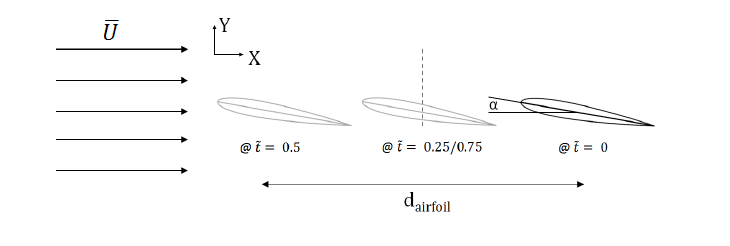
\includegraphics[width=0.8\textwidth]{figures/Setup/Setup.png}
\caption{Schematic of the surging airfoil problem}
\label{fig:SetUpSketch}
\end{figure}

The airfoil motion is set as follows
\begin{equation}
\label{eq:displacement}
  d_{airfoil} = A cos(2\pi f t) =  Acos(2\pi t/T) = Acos(2\pi\tilde{t})
\end{equation}

\noindent where $A$ is the amplitude and $T=1/f$ is the time period of the oscillation.
The variable $\tilde{t}$ is the fractional part in the oscillation cycle and is defined as $\tilde{t}=\{t/T\} = t/T - \lfloor t/T \rfloor$ (where $\lfloor \cdot \rfloor$ is the floor function).

The (non-dimensional) relative velocity is expressed as
\begin{equation}
\label{eq:relVelocity}
  \tilde{U}_{rel} = U_{rel}/U_\infty = 1 - U_{airfoil}/U_\infty = (1+\mu_{sect} sin(2\pi\tilde{t}))
\end{equation}
\noindent where $\mu_{sect}$ is the sectional advance ratio.
Note that for a sectional advance ratio above $1.0$ a negative relative velocity or a reversed flow condition is attained (e.g., at this radial section/location of the blade).
Under the reversed flow condition the relative flow is from the (geometric) trailing edge to the leading edge of the airfoil.

At $\tilde{t}$=0, with $\psi$=$0^\circ$ or $\psi$=$0^\circ$ (where, $\psi$ is the phase in the oscillation cycle and $\psi$ is the azimuthal position of the blade), the relative velocity is the free-stream velocity (i.e., $U_\infty$).
The same holds at $\tilde{t}$=0.5 or $\psi$=$180^\circ$.
At $\tilde{t}$=0.25 or $\psi$=$90^\circ$, the airfoil is at the maximum relative velocity and at $\tilde{t}$=0.75 or $\psi$=$270^\circ$ is at the minimum relative velocity.
Advancing part of the cycle is defined between $\tilde{t}$=0 or $\psi$=$0^\circ$ and $\tilde{t}$=0.5 or $\psi$=$180^\circ$, while retreating part is between $\tilde{t}$=0.5 or $\psi$=$180^\circ$ and $\tilde{t}$=1.0 or $\psi$=$360^\circ$ (or back to $\psi$=$0^\circ$).

The free-stream or mean Reynolds number is defined as: $Re=U_\infty C/\nu$, where $C$ is the chord.
The reduced frequency is defined as $k=\pi f C/U_\infty$ while the amplitude is related as $A = \frac{\mu_{sect} C}{2k}$.

\section{Summary of Cases}
\label{sec:baseline_case_summary}

In the current study, the reduced frequency is held fixed at $k$=0.133 while three Reynolds numbers of $Re$=40,000, 200,000 and 1,000,000 are considered together with two sectional advance ratios of $\mu_{sect}$=1.0 and 1.2, i.e., six cases are considered in total.
The angle of attack of the airfoil is set to 6$^\circ$.
Note that we considered the Reynolds number of $Re$=40,000 in a previous study~\cite{bib:kocher_scitech2017} that was selected in accordance with the experiments conducted in \cite{bib:granlund2016} where the airfoil was placed in a constant flow and oscillated in the streamwise direction.
The six cases are summarized in Table~\ref{table:summary_cases}.

\begin{table}[H]
\centering
\caption{Summary of surging cases for LES}
\label{table:summary_cases}
\begin{tabular}{|l|c|c|c|c|}
\hline
Airfoil   & $\alpha$ & $k$ & $\mu_{sect}$ & $Re$ \\
\hline
\hline
NACA 0012 & 6$^\circ$ & $0.133$ & \{1.0, 1.2\} & \{40,000,\; 200,000,\; 1,000,000\} \\
\hline
\end{tabular}
\end{table}

The computational domain is set to be $100C$ x $50C$ x $0.2C$.
At the inlet, a constant free-stream velocity is applied
(note that the airfoil is moved sinusoidally in the streamwise direction).
No-slip condition is prescribed on the moving airfoil.
The top and bottom surfaces are set as slip walls.
Side surfaces in the spanwise direction (i.e., front and back surfaces) are imposed to be periodic.
A natural pressure condition is used at the outlet.
A second-order implicit time integration scheme, e.g., see \cite{bib:tran2017b}, is employed with about 1,440 steps in an oscillation cycle.

%TODO: give justification for this mesh ... typical LES resolution for a BL (based on highest Reynolds number in the surge cycle) ... but indicate no consideration taken for other flow features such as separation and LEV.
An unstructured hybrid/boundary layer mesh is used.
The mesh is comprised of hex and wedge elements which is generated by first generating a mesh on the front surface and by subsequently applying an extrusion in the spanwise direction. This (non-adapted) mesh is used for all cases listed above. Again, this is done to get familiar with the features of the current problem at different conditions, while mesh adaptivity is investigated in the next chapter. The non-adapted mesh is constructed by following recommended practices in terms of mesh resolution on the surface of the airfoil and around it, as discussed below.

Refinement zones are placed around the airfoil to resolve the flow structures of interest, see Figure \ref{fig:mesh} (where three refinement zones are noted).
In the finest refinement zone (Z1), mesh size is set to be $C/256$.
In the subsequent two zones (Z2 and Z3), it is set to be $C/128$ and $C/64$, respectively.
In the spanwise direction, 50 extruded elements are used.
A layered and graded mesh (with geometric growth) is used around the airfoil surface, see Figure \ref{fig:mesh2}.
The first layer height is set to be $\mathcal{O}(10^{-5} C)$ such that it is below 1 in wall units for all cases.
Similarly, mesh spacing/resolution on the airfoil surface in the streamwise and spanwise directions is set to be below 80 and 50 in wall units, respectively, for $Re=40,000$ and $200,000$, and about 200 in wall units for $Re=1,000,000$. These are determined for the phase with the maximum relative velocity or instantaneous Reynolds number (i.e., $\psi=90^\circ$). Note that the surface mesh resolution is on the higher/coarser side for the highest Reynolds number of $Re=1,000,000$, however, it is sufficient for an initial non-adapted mesh used here to get familiar with the features of the current problem.
Overall the mesh contains about 6.2 million nodes and 10.8 million elements.

\begin{figure}[H]
\centering
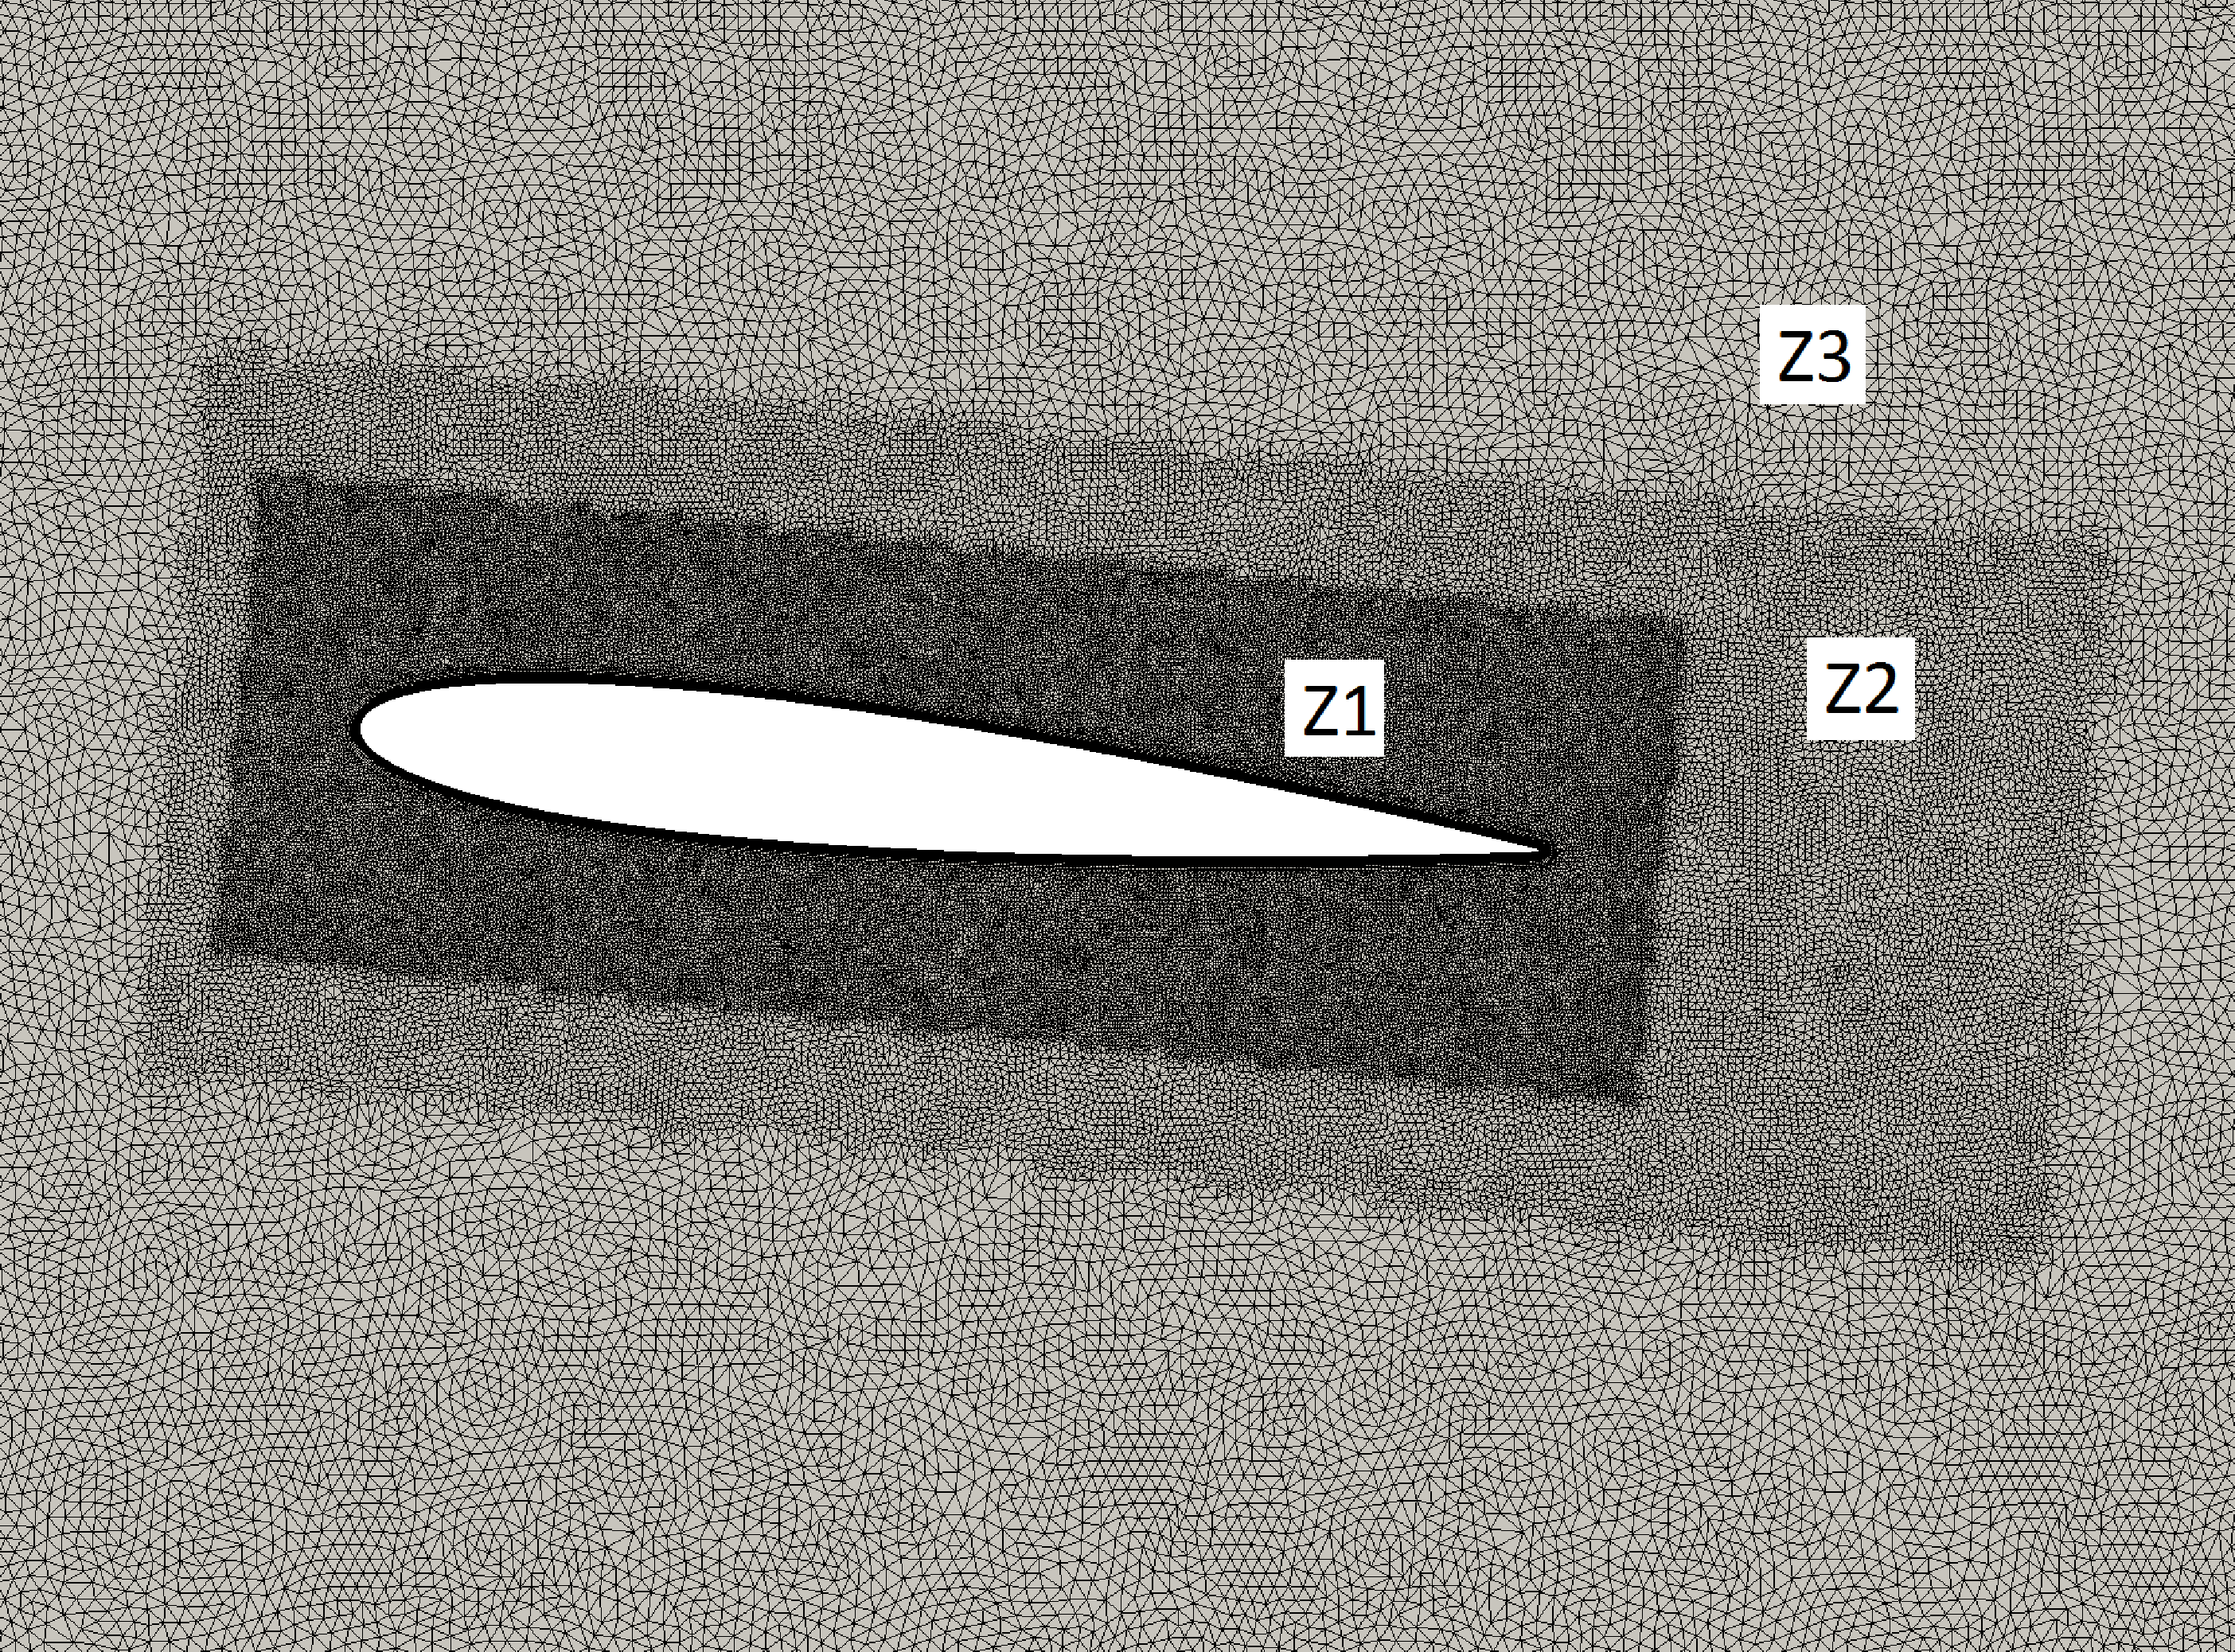
\includegraphics[width=0.7\textwidth]{figures/Setup/mesh_screenshot.pdf}
\caption{Mesh around the airfoil with refinement zones}
\label{fig:mesh}
\end{figure}

\begin{figure}[H]
\centering
\includegraphics[width=0.45\textwidth]{figures/Setup/mesh_LE.pdf}
\includegraphics[width=0.45\textwidth]{figures/Setup/mesh_TE.pdf}
\caption{Layered and graded mesh around the leading edge and trailing edge of the airfoil}
\label{fig:mesh2}
\end{figure}

\section{Results and Discussion}

\subsection{Force Response}

\begin{figure}[H]
	\begin{subfigure}{0.5\textwidth}
		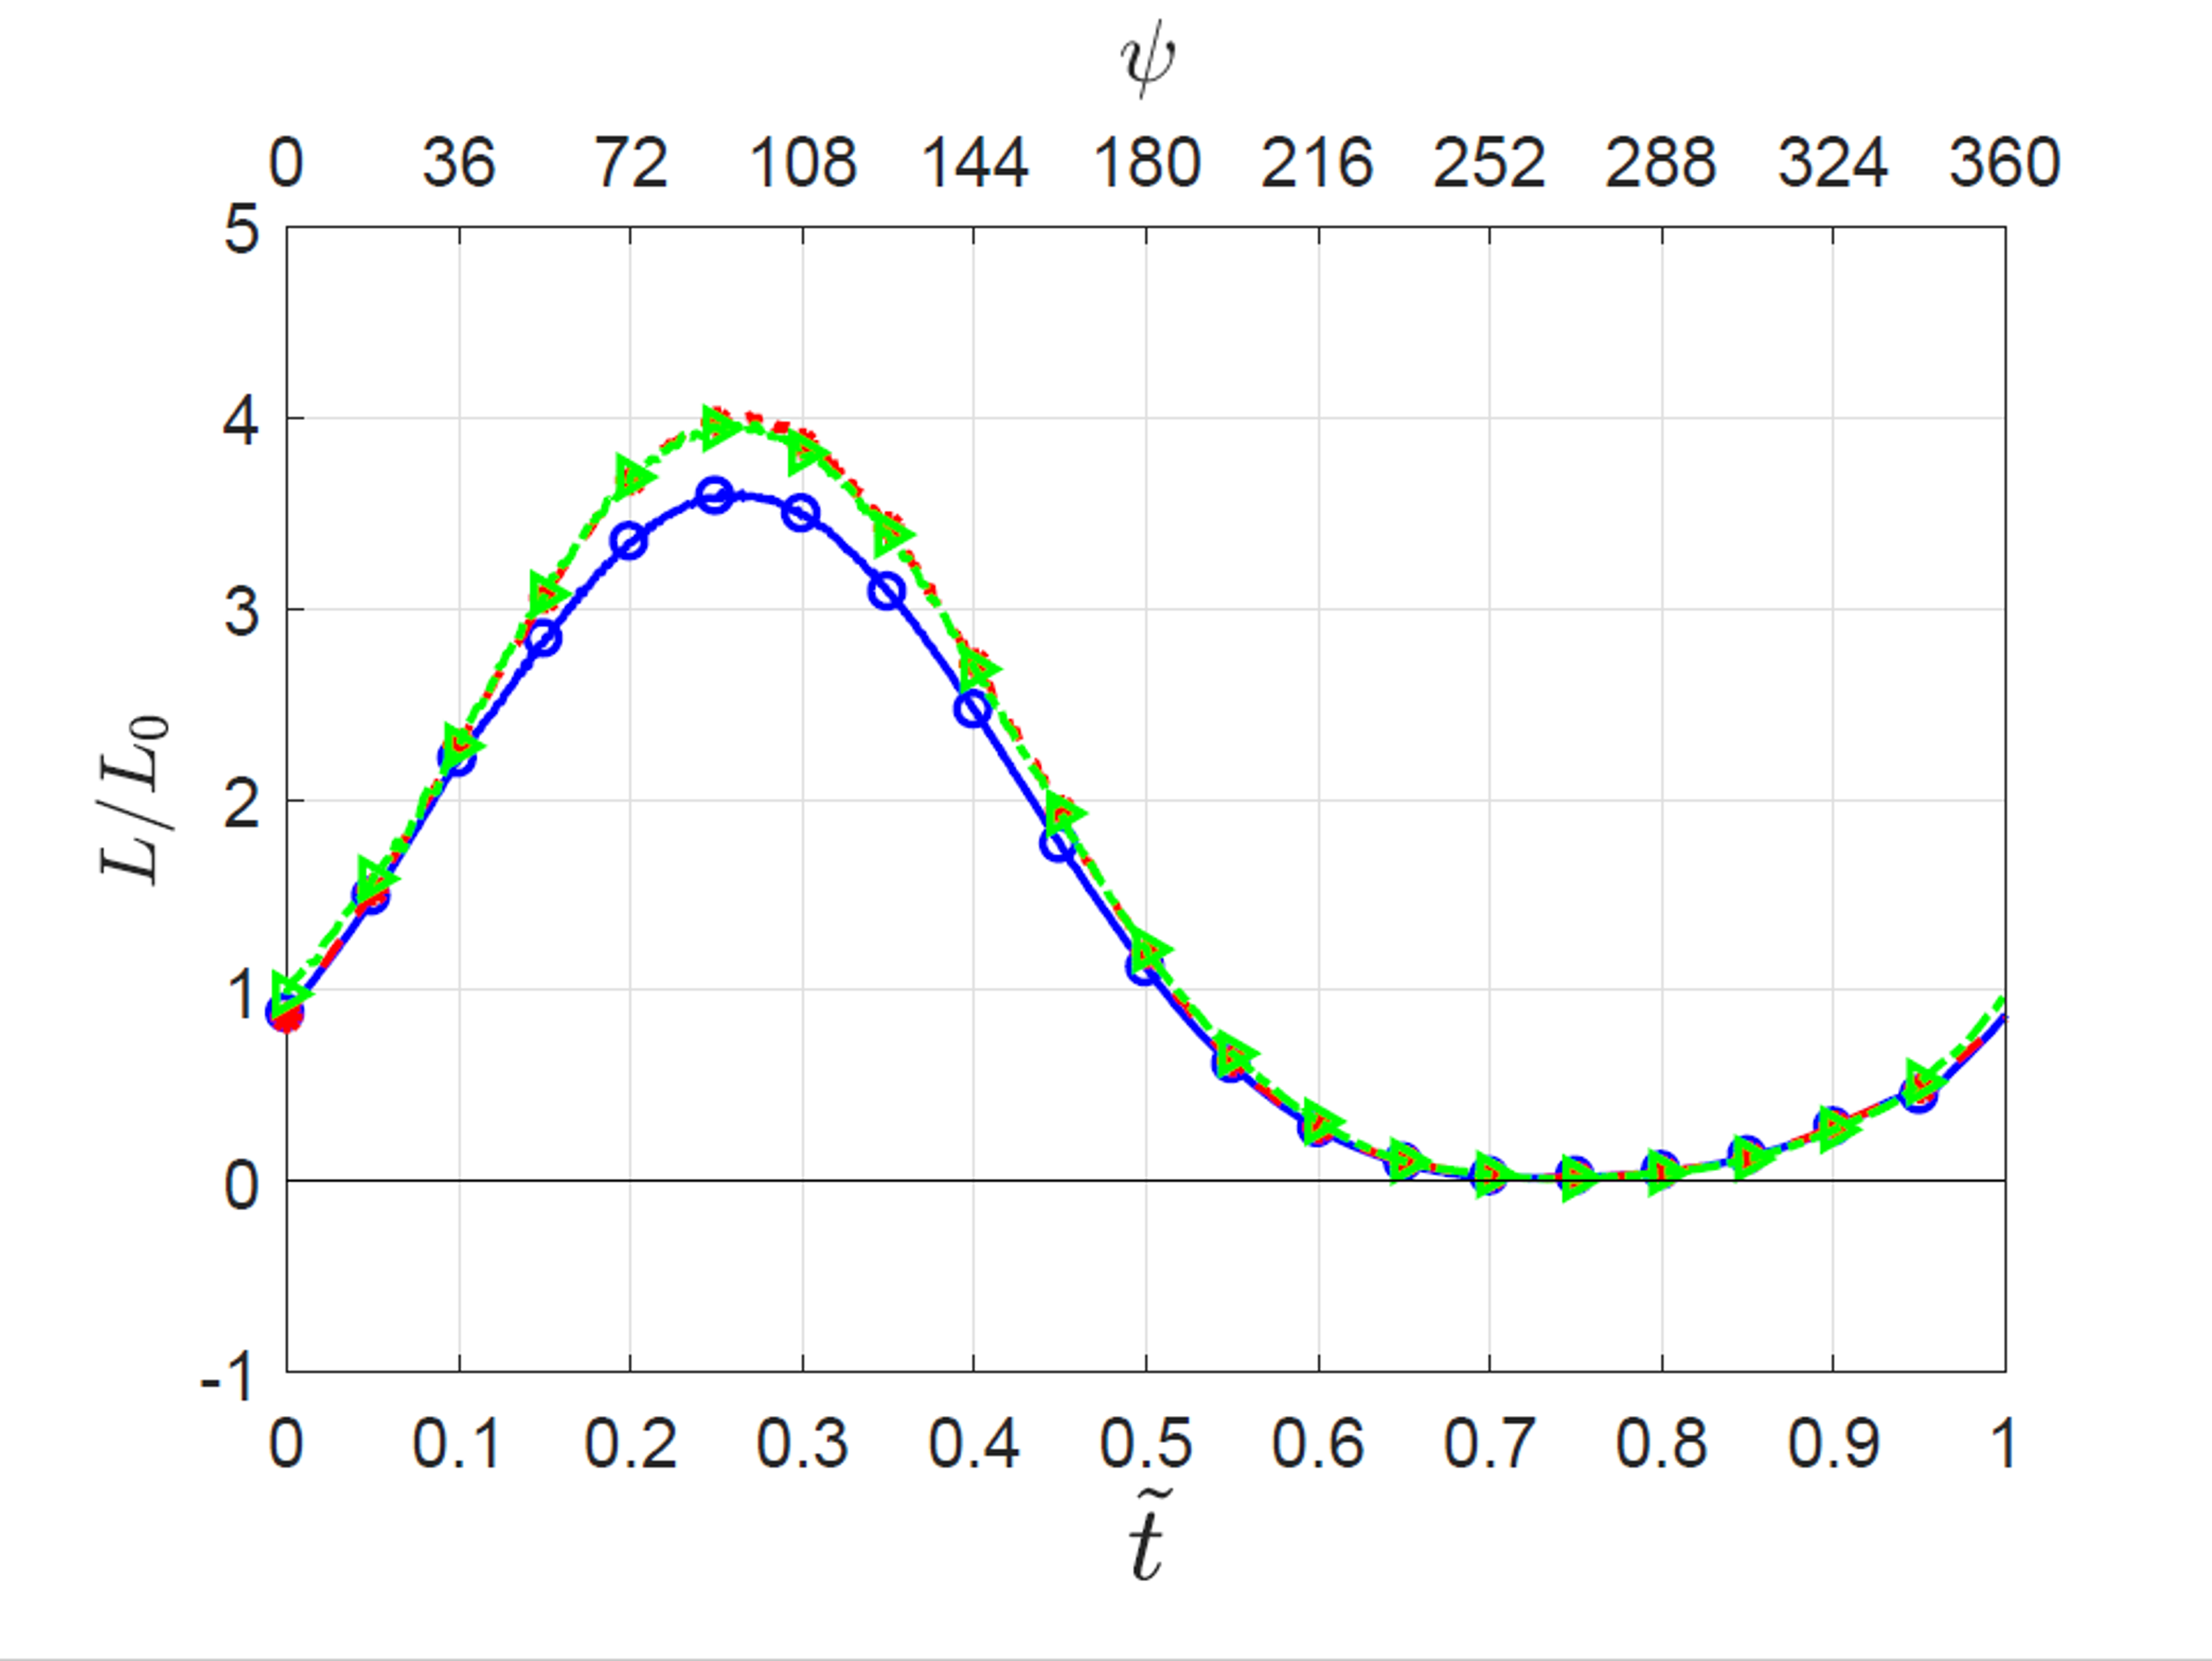
\includegraphics[width=1\textwidth]{figures/lift_Re_effect_lambda_1pt0.png}
		\subcaption{$\mu_{sect} = 1.0$}
		\label{fig:lift_Re_comparision_lambda_1p0}
	\end{subfigure}
 	\begin{subfigure}{0.5\textwidth}
		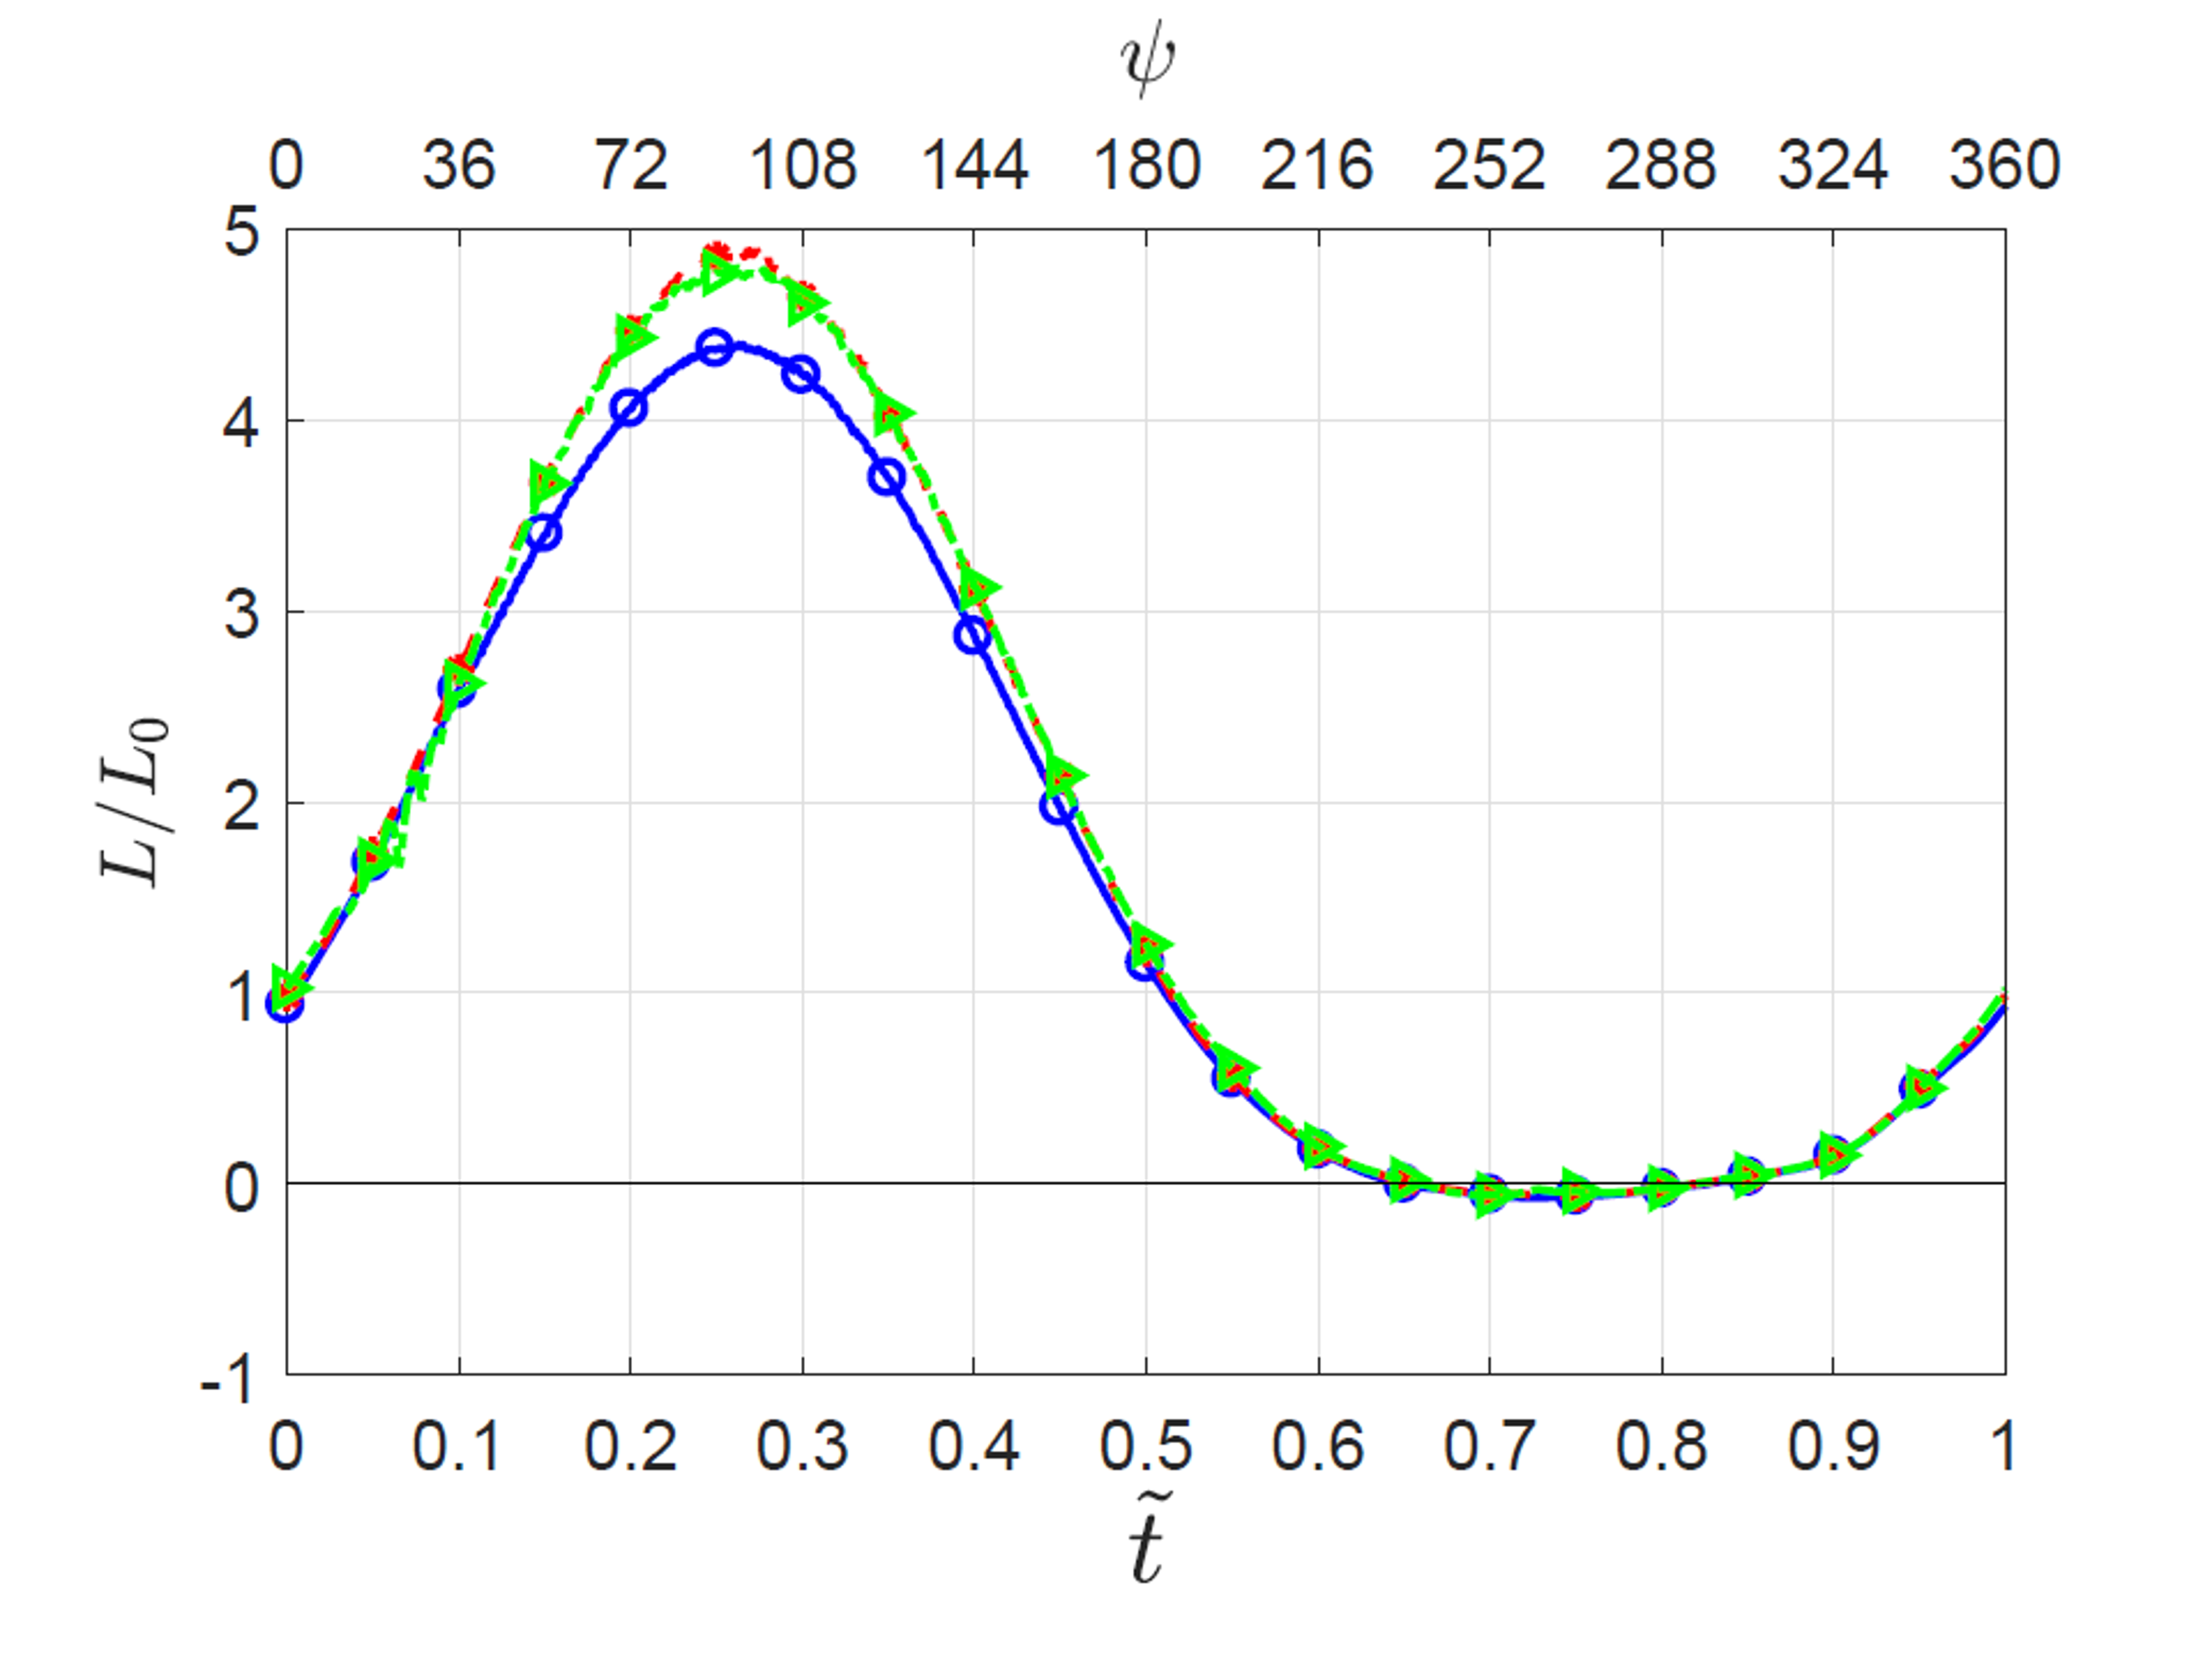
\includegraphics[width=1\textwidth]{figures/lift_Re_effect_lambda_1pt2.png}
        \subcaption{$\mu_{sect} = 1.2$}
		\label{fig:lift_Re_comparision_lambda_1p2}
	\end{subfigure}

 	\caption{Normalized lift force for $Re$=40,000 (green line with open triangles), 200,000 (red line with solid circles) and 1,000,000 (blue line with open circles) at $\mu_{sect}$=1.0 and 1.2}
 	\label{fig:lift_comparison}
\end{figure}

Lift force is shown in Figure \ref{fig:lift_comparison}.
Lift is normalized by its static counterpart, i.e., $L_0$ is the average or steady lift for the static airfoil at the mean Reynolds number over the surging cycle.
This normalization was used in our previous study with $Re$=40,000~\cite{bib:kocher_scitech2017} to compare against the experimental data of \cite{bib:granlund2016}, where a good agreement was shown between the experimental and simulation data.
Data is phase averaged over 4 cycles.
%%%We note that the averaged drag data exhibits fluctuations which is due to the presence of a turbulent flow, especially during the advancing phase of the cycle with a higher relative velocity or Reynolds number.
%%%However, these fluctuations are marginal in nature and averaging over additional cycles will be useful.

Overall, the lift force follows a similar qualitative trend for all the cases.
Maximum lift is achieved at $\tilde{t}=0.25$, which is expected as the airfoil achieves maximum relative velocity at that point.
After $\tilde{t}=0.25$, the lift starts decreasing as the airfoil begins to decelerate and enters the retreating phase. 
The lift keeps decreasing till about $\tilde{t}=0.65$ and plateaus or reaches a value close to zero during the middle of the retreating phase (i.e., around $\tilde{t}=0.75$ when the airfoil is at its minimum relative velocity).
We note that for both advance ratios of $\mu_{sect}$=1.0 and 1.2 a zero relative velocity is attained and for the higher advance ratio of $\mu_{sect}$=1.2 the relative velocity also becomes negative.
Lift starts to recover after $\tilde{t}=0.75$ as the airfoil starts accelerating again.
For each advance ratio, the normalized lift during the advancing phase for $Re$=1,000,000 is slightly smaller compared to the other two Reynolds numbers, see Figure \ref{fig:lift_Re_comparision_lambda_1p0} or Figure \ref{fig:lift_Re_comparision_lambda_1p2}.
The normalized lift is very similar between $Re$=40,000 and 200,000 cases.
The peak normalized lift is about 9\% lower for the highest Reynolds number case as compared to the lower Reynolds number cases for each advance ratio.
On the other hand, for a given Reynolds number the normalized lift is higher for the higher advance ratio, which is expected due to the higher dynamic pressure in any given instance or phase in the surging cycle.
The peak normalized lift is about 21\% higher for the higher advance ratio case as compared to the lower advance ratio case for each Reynolds number, which is the difference in the peak dynamic pressure between the two advance ratios.

\subsection{Flowfield: Spanwise Vorticity}

In this section, we present spanwise vorticity over the cycle at 8 different phases of $\psi$ = $195^\circ$, $225^\circ$, $240^\circ$, $255^\circ$, $270^\circ$, $315^\circ$, $330^\circ$,and $345^\circ$, which are all in the retreating part of the surging cycle.
We focus our attention on the leading edge vortex (LEV) which is the dominant flow feature.
It forms and advects during the retreating part, while in the advancing part the flow remains attached.
As noted earlier, data is phase averaged over 4 cycles.
In addition, averaging is also applied in the spanwise direction.

Figure \ref{fig:vortScreen_1pt0} shows the spanwise vorticity for the lower advance ratio of $\mu_{sect}$=1.0.
The voriticy range is selected to be [-10,10]$\times U_\infty /C$.
At $\psi$=$195^\circ$, the flow over the airfoil is mostly attached, however, the boundary layer is relatively thick as the airfoil is decelerating, see Figures~\ref{fig:Re_40k_1pt0_phi195}, \ref{fig:Re_200k_1pt0_phi195} and \ref{fig:Re_1m_1pt0_phi195}.
As expected, the boundary layer is much thicker for the lowest Reynolds number of $Re$=40,000 as compared to the other two higher Reynolds numbers.

\begin{figure}[H]
	\centering
	
	\begin{subfigure}[b]{0.32\textwidth}
		\centering
		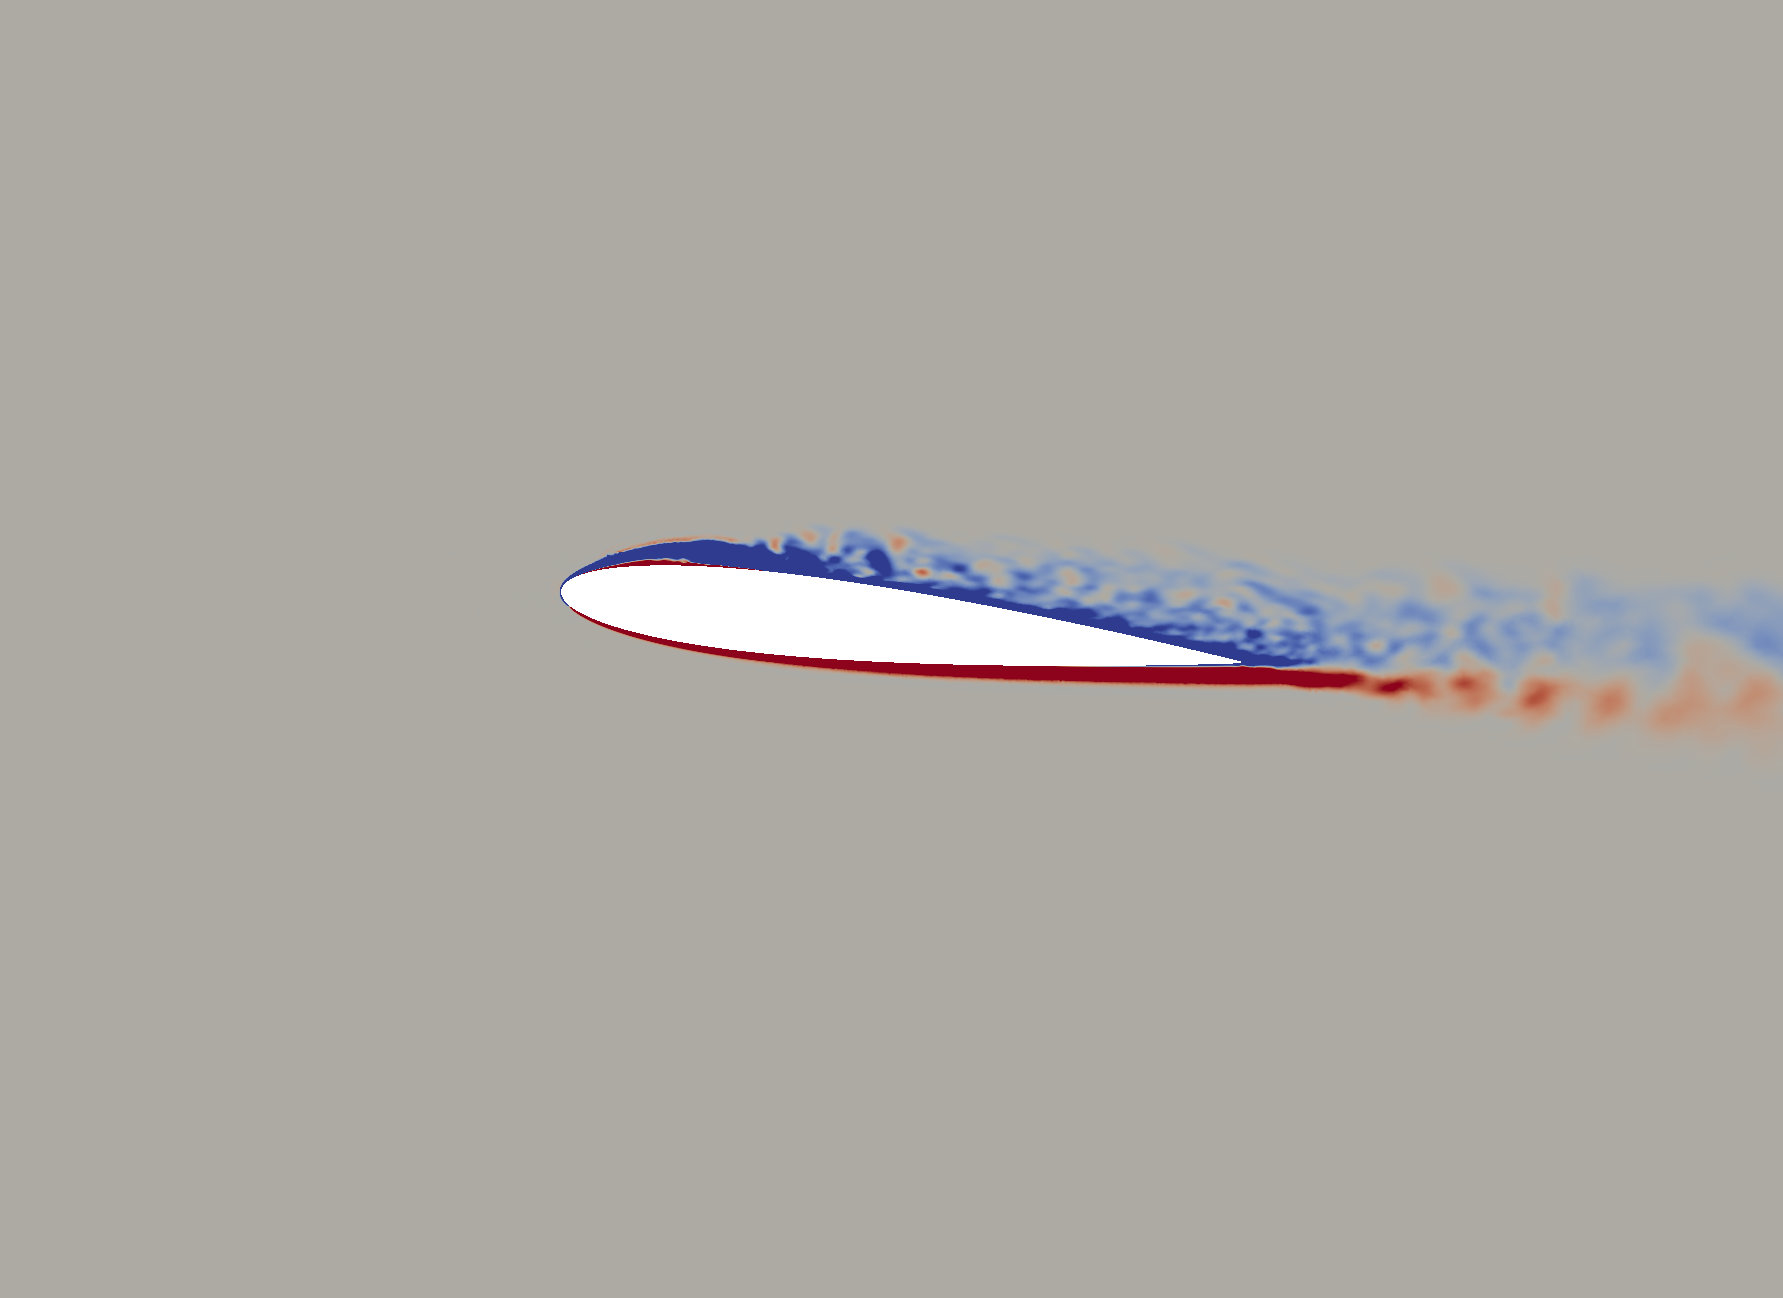
\includegraphics[width=1\textwidth]{figures/Vorticity_plots/Re_40k_1pt0/phase_195.png}
		\caption{$Re=4e4$, $\psi$ = $195^\circ$, $\tilde{t}=0.542$}
		\label{fig:Re_40k_1pt0_phi195}
	\end{subfigure}
	\begin{subfigure}[b]{0.32\textwidth}
		\centering
		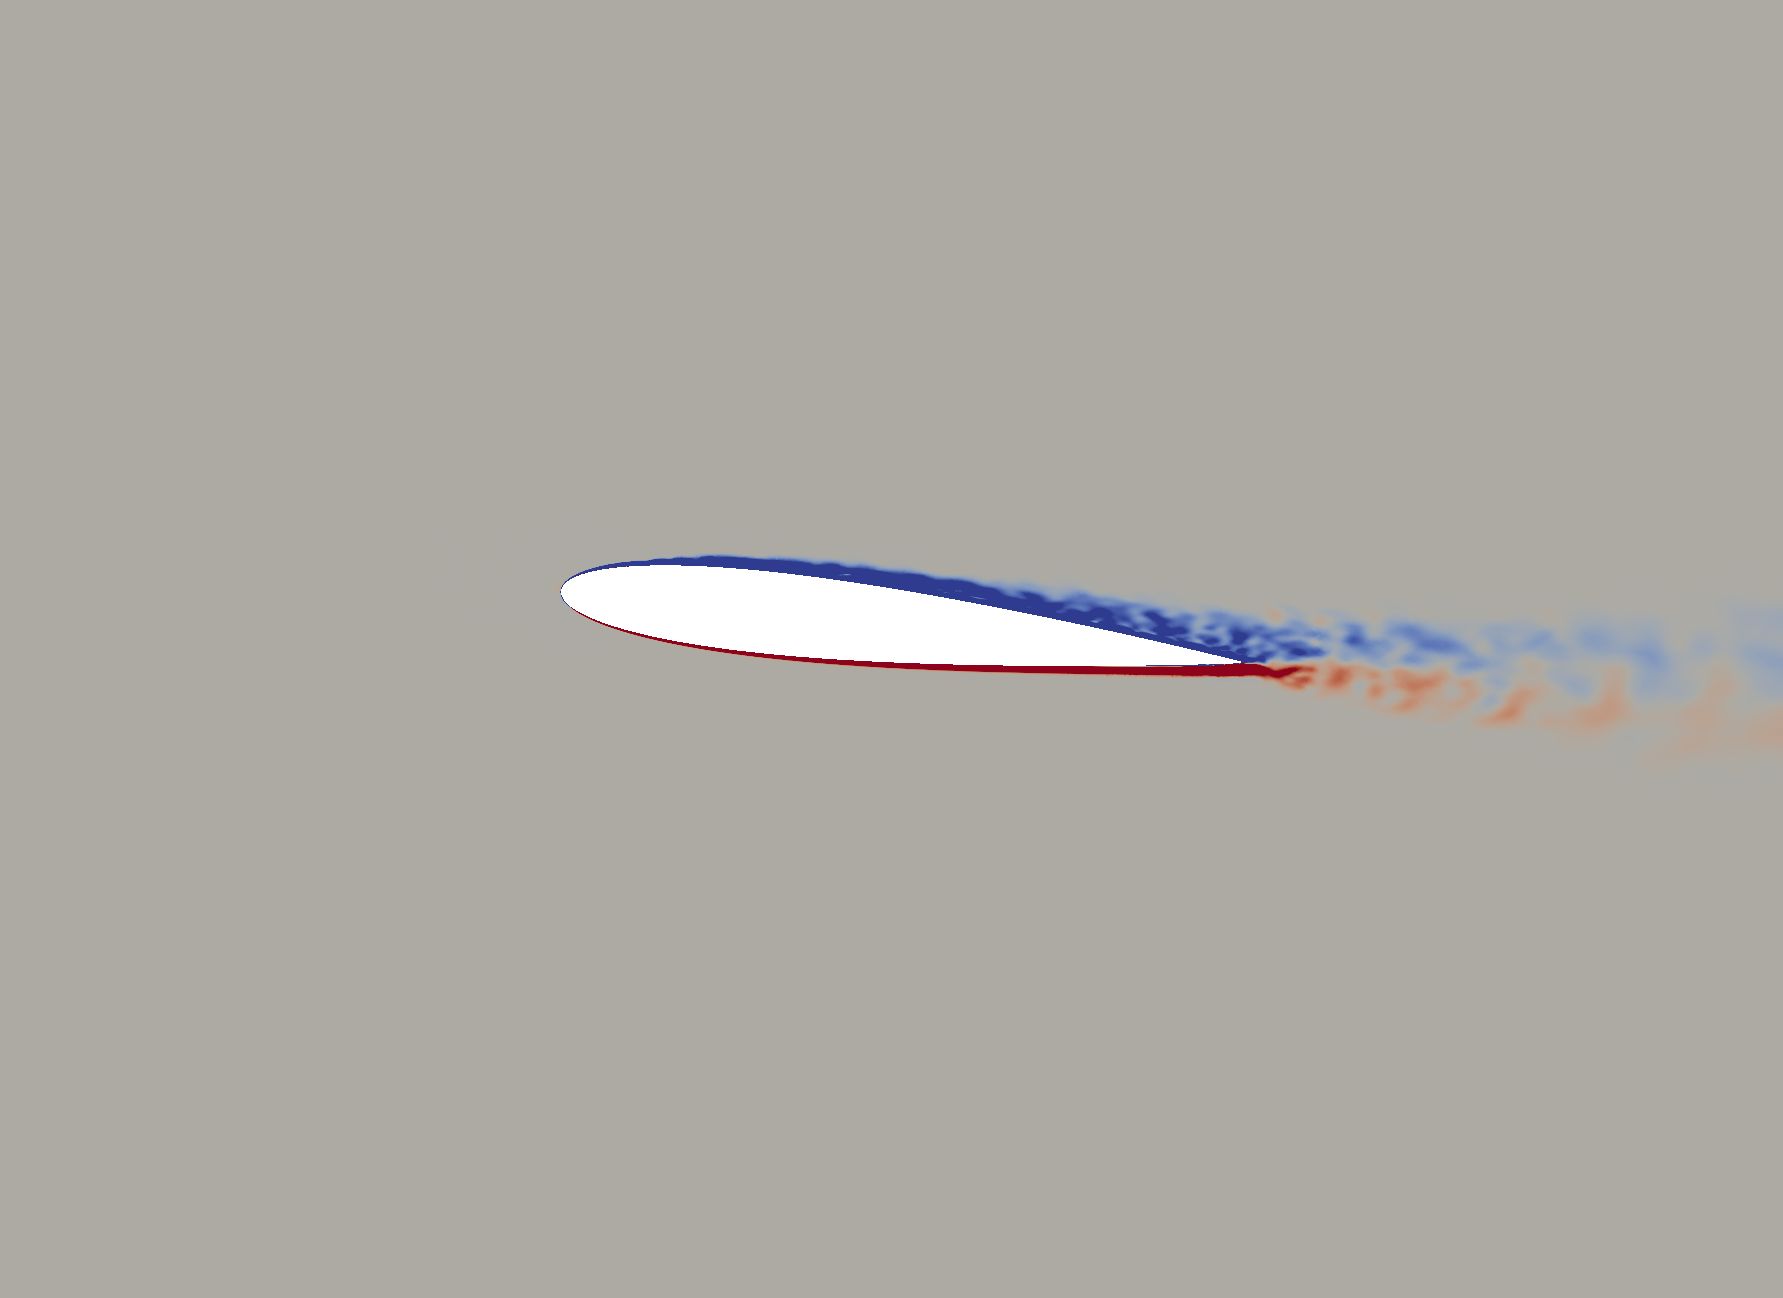
\includegraphics[width=1\textwidth]{figures/Vorticity_plots/Re_200k_1pt0/phase_195.png}
		\caption{$Re=2e5$, $\psi$ = $195^\circ$, $\tilde{t}=0.542$}
		\label{fig:Re_200k_1pt0_phi195}
	\end{subfigure}
	\begin{subfigure}[b]{0.32\textwidth}
		\centering
		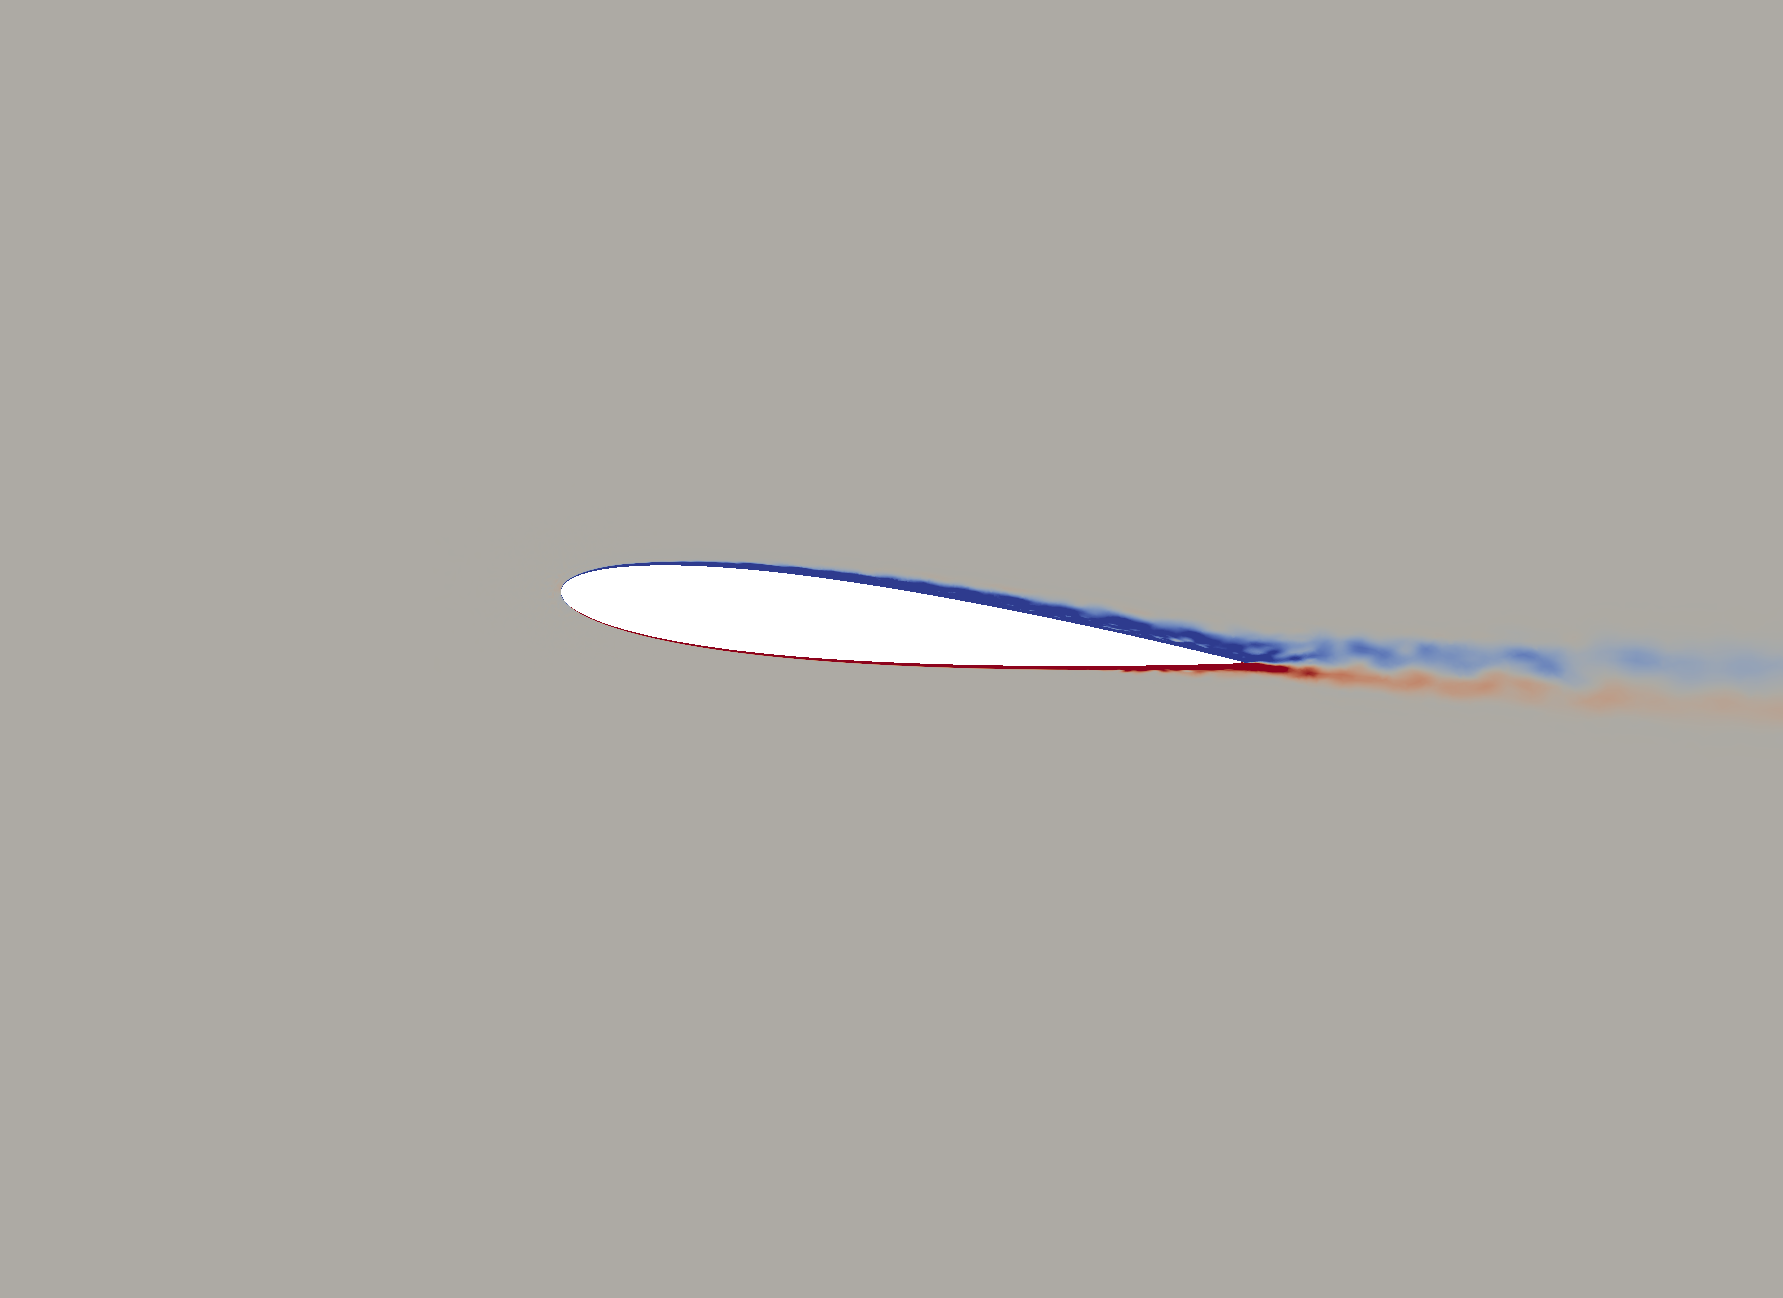
\includegraphics[width=1\textwidth]{figures/Vorticity_plots/Re_1m_1pt0/phase_195.png}
		\caption{$Re= 1e6$, $\psi$ = $195^\circ$, $\tilde{t}=0.542$}
		\label{fig:Re_1m_1pt0_phi195}
	\end{subfigure}
	
	\begin{subfigure}[b]{0.32\textwidth}
		\centering
		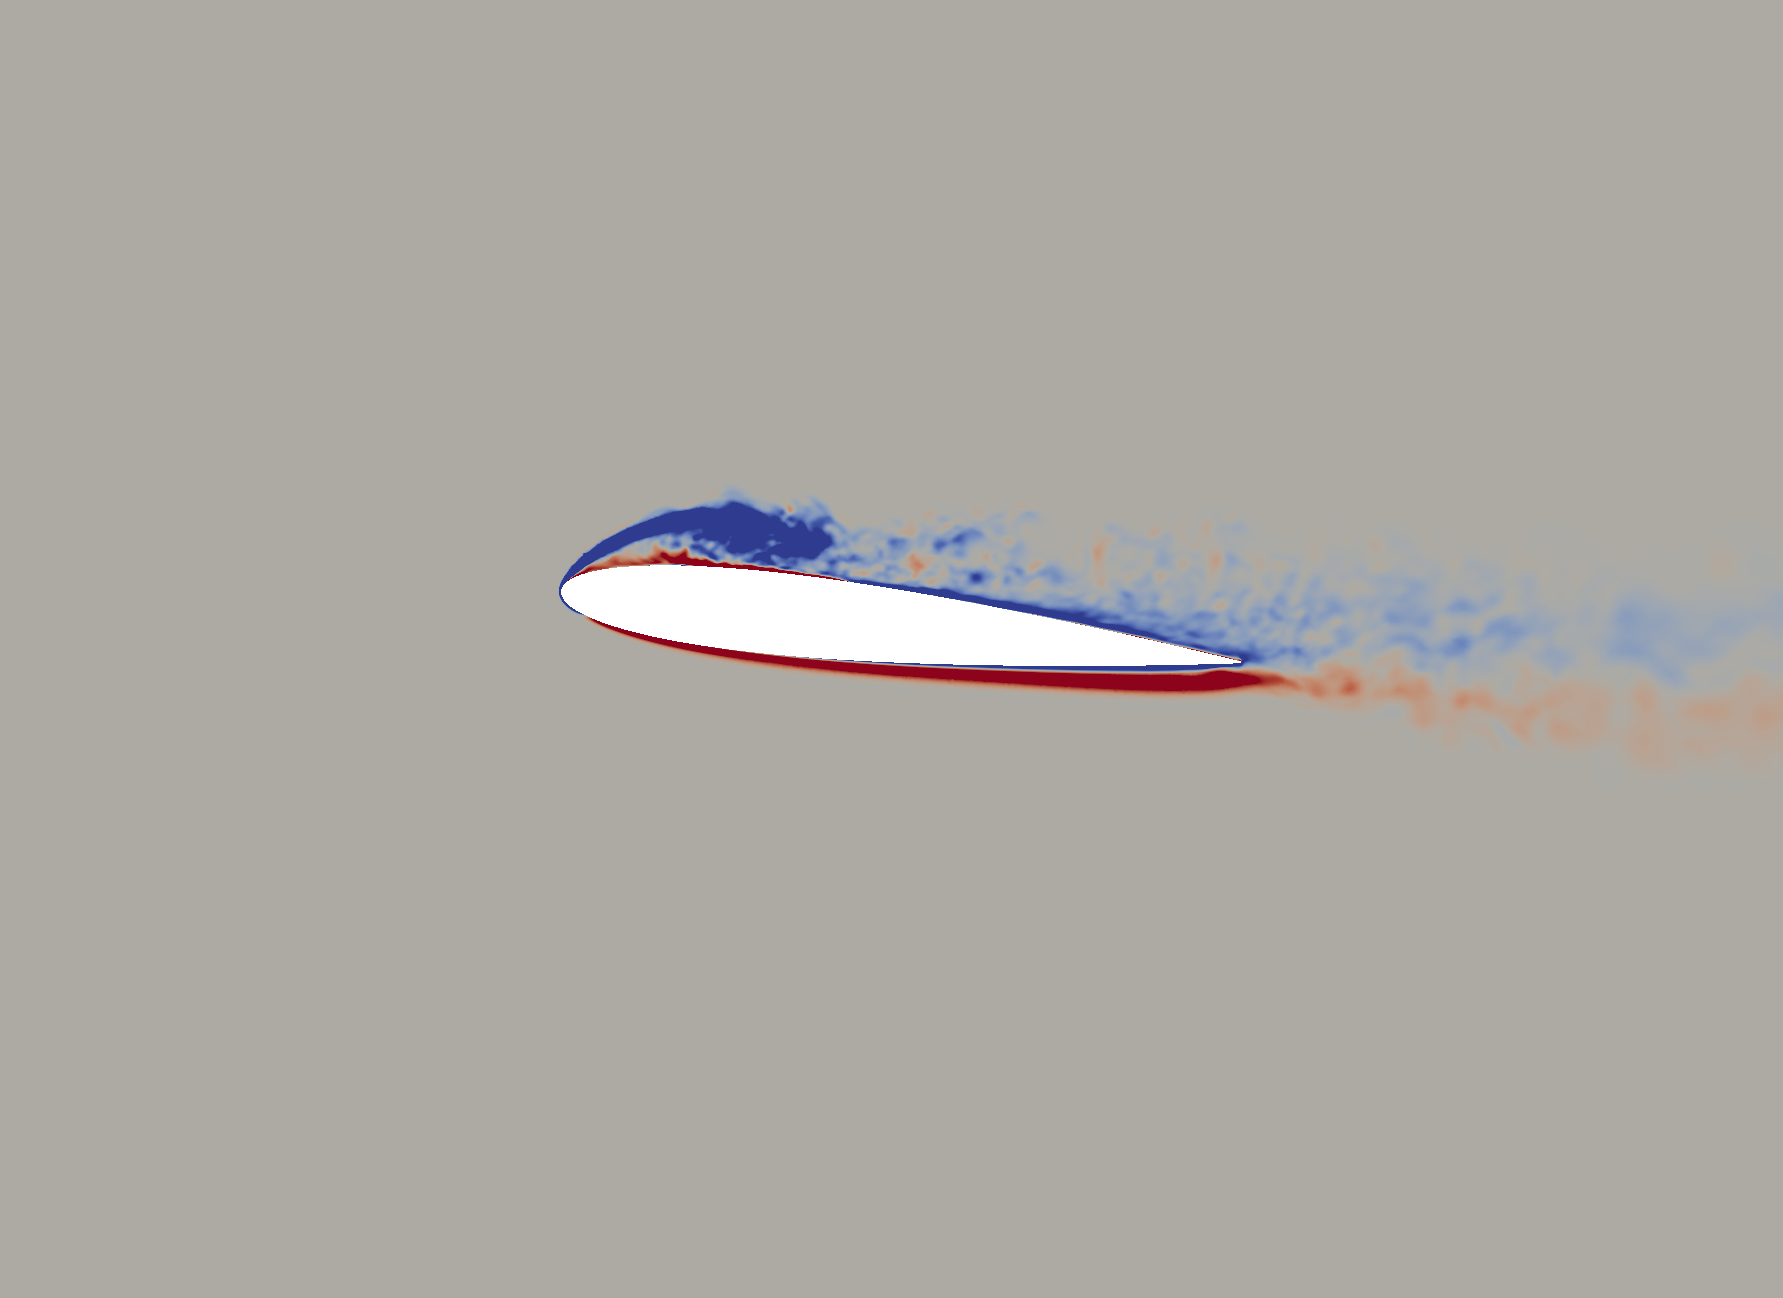
\includegraphics[width=1\textwidth]{figures/Vorticity_plots/Re_40k_1pt0/phase_225.png}
		\caption{$Re=4e4$, $\psi$ = $225^\circ$, $\tilde{t}=0.625$}
		\label{fig:Re_40k_1pt0_phi225}
	\end{subfigure}
	\begin{subfigure}[b]{0.32\textwidth}
		\centering
		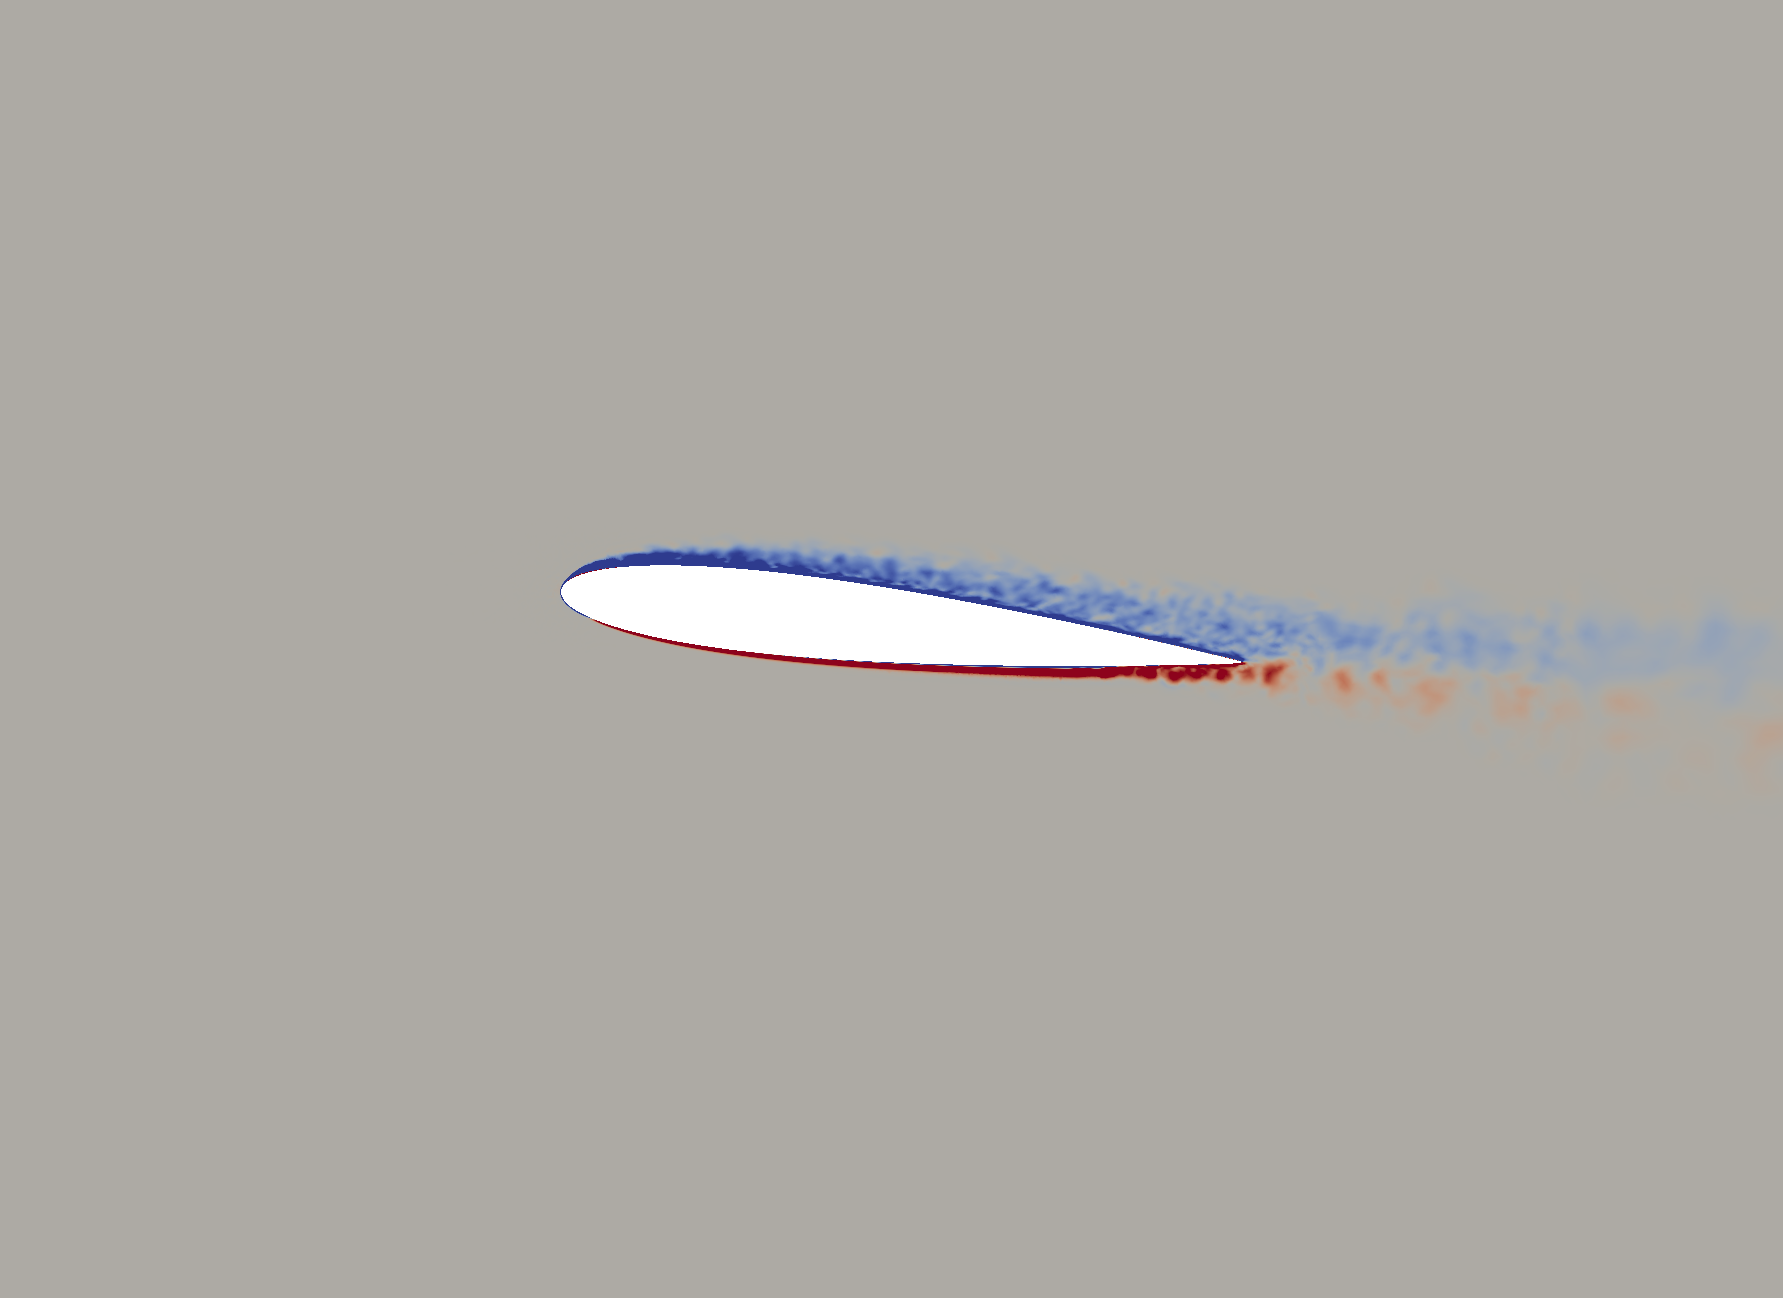
\includegraphics[width=1\textwidth]{figures/Vorticity_plots/Re_200k_1pt0/phase_225.png}
		\caption{$Re=2e5$, $\psi$ = $225^\circ$,  $\tilde{t}=0.625$}
		\label{fig:Re_200k_1pt0_phi225}
	\end{subfigure}
	\begin{subfigure}[b]{0.32\textwidth}
		\centering
		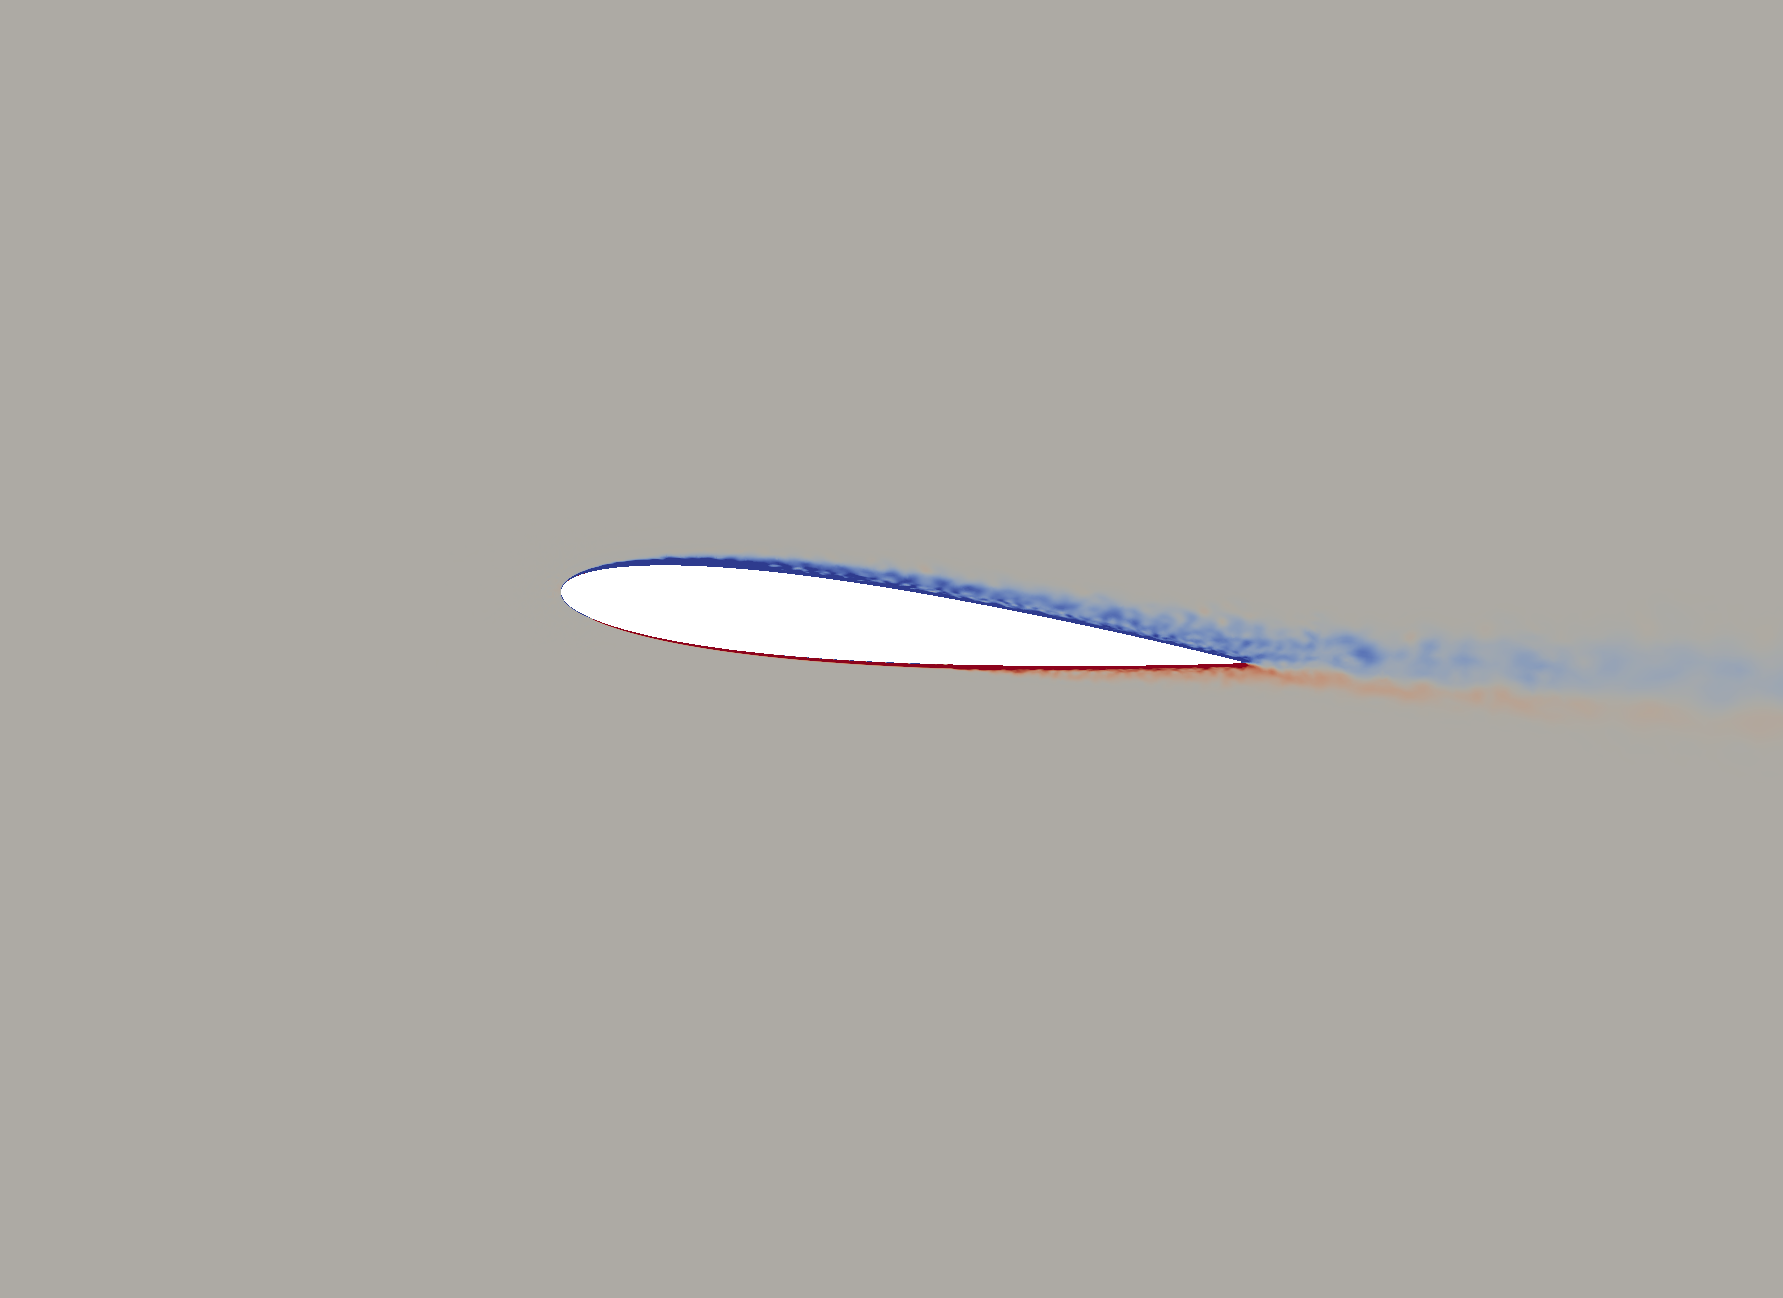
\includegraphics[width=1\textwidth]{figures/Vorticity_plots/Re_1m_1pt0/phase_225.png}
		\caption{$Re=1e6$, $\psi$ = $225^\circ$,  $\tilde{t}=0.625$}
		\label{fig:Re_1m_1pt0_phi225}
	\end{subfigure}
	
	\begin{subfigure}[b]{0.32\textwidth}
		\centering
		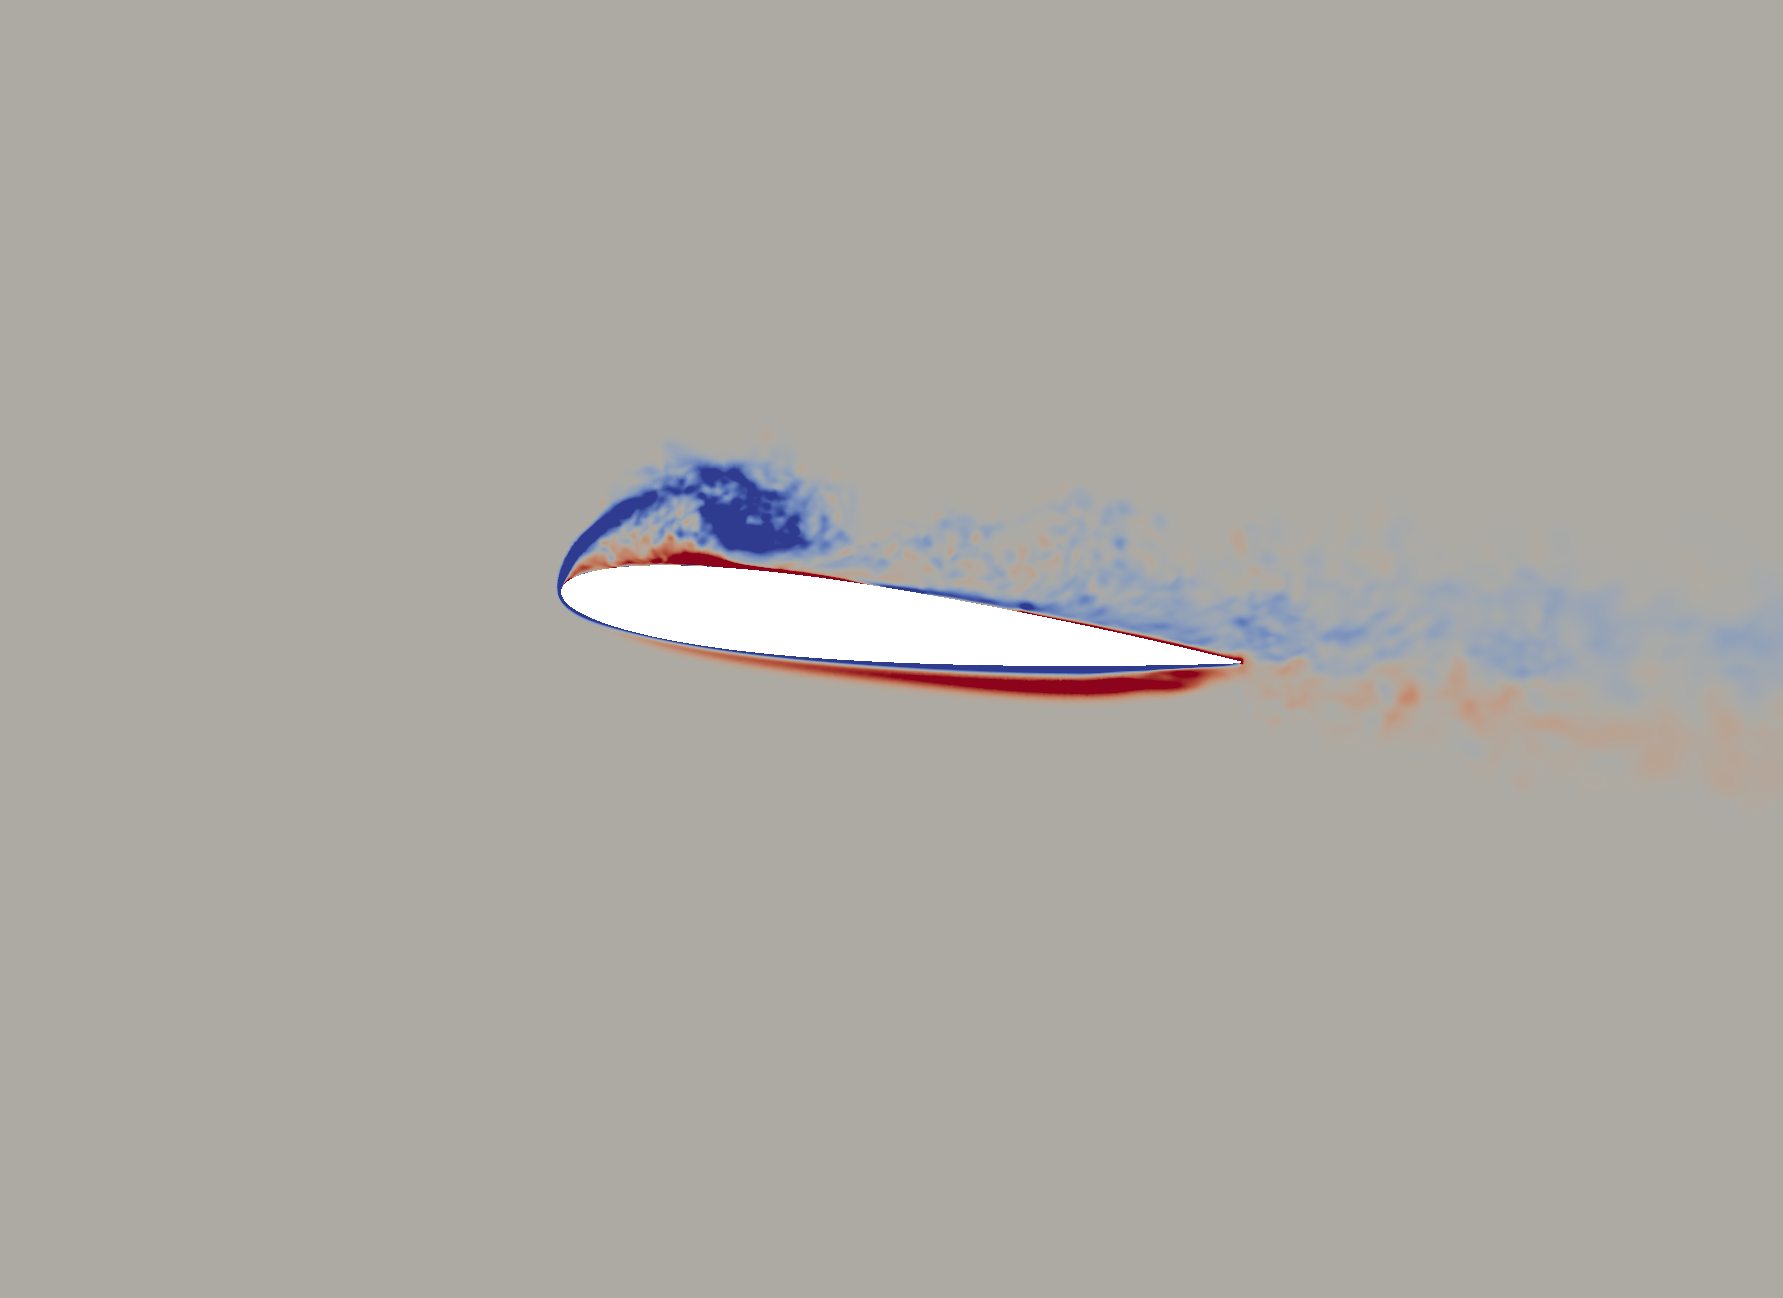
\includegraphics[width=1\textwidth]{figures/Vorticity_plots/Re_40k_1pt0/phase_240.png}
		\caption{$Re=4e4$, $\psi$ = $240^\circ$, $\tilde{t}=0.667$}
		\label{fig:Re_40k_1pt0_phi240}
	\end{subfigure}
	\begin{subfigure}[b]{0.32\textwidth}
		\centering
		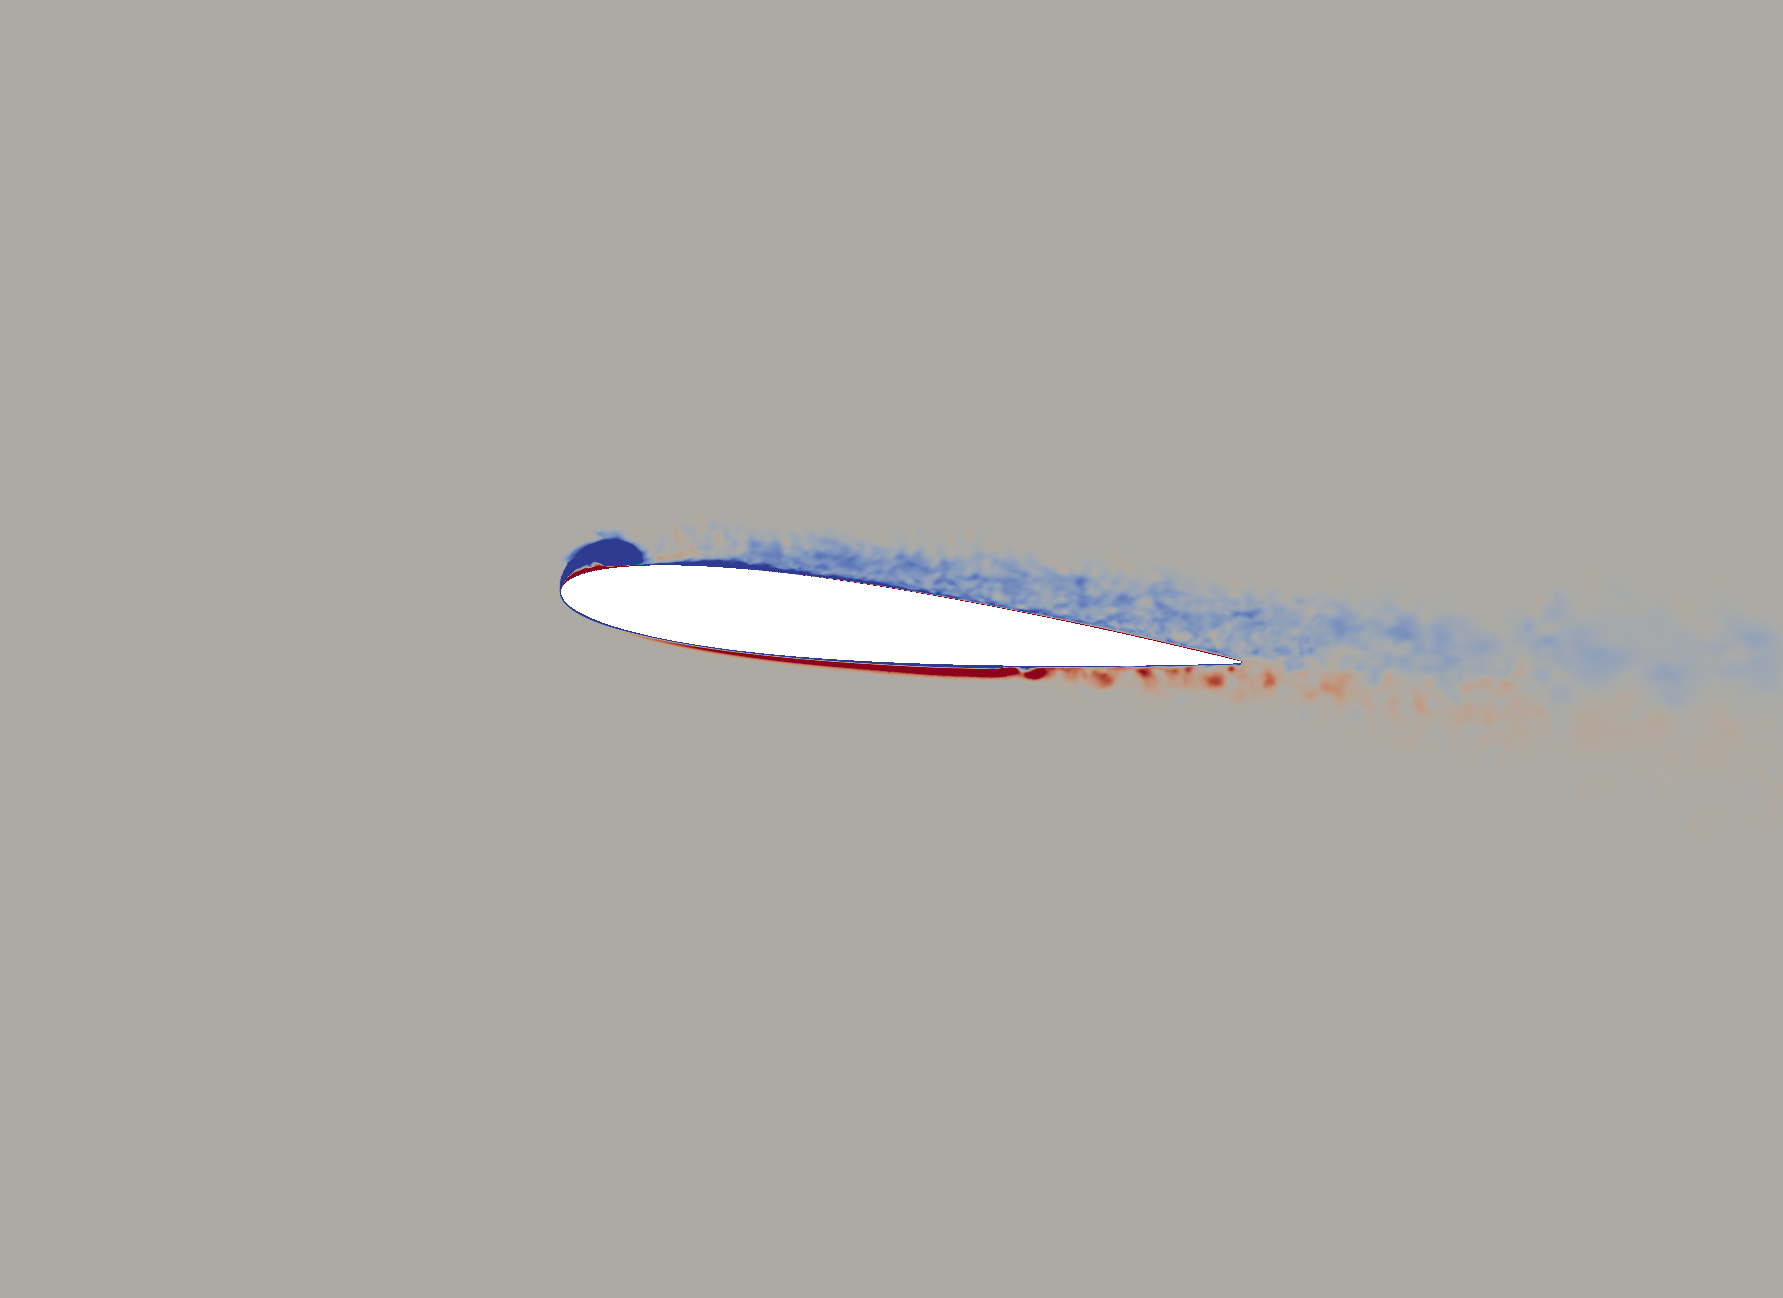
\includegraphics[width=1\textwidth]{figures/Vorticity_plots/Re_200k_1pt0/phase_240.png}
		\caption{$Re=2e5$, $\psi$ = $240^\circ$, $\tilde{t}=0.667$}
		\label{fig:Re_200k_1pt0_phi240}
	\end{subfigure}
	\begin{subfigure}[b]{0.32\textwidth}
		\centering
		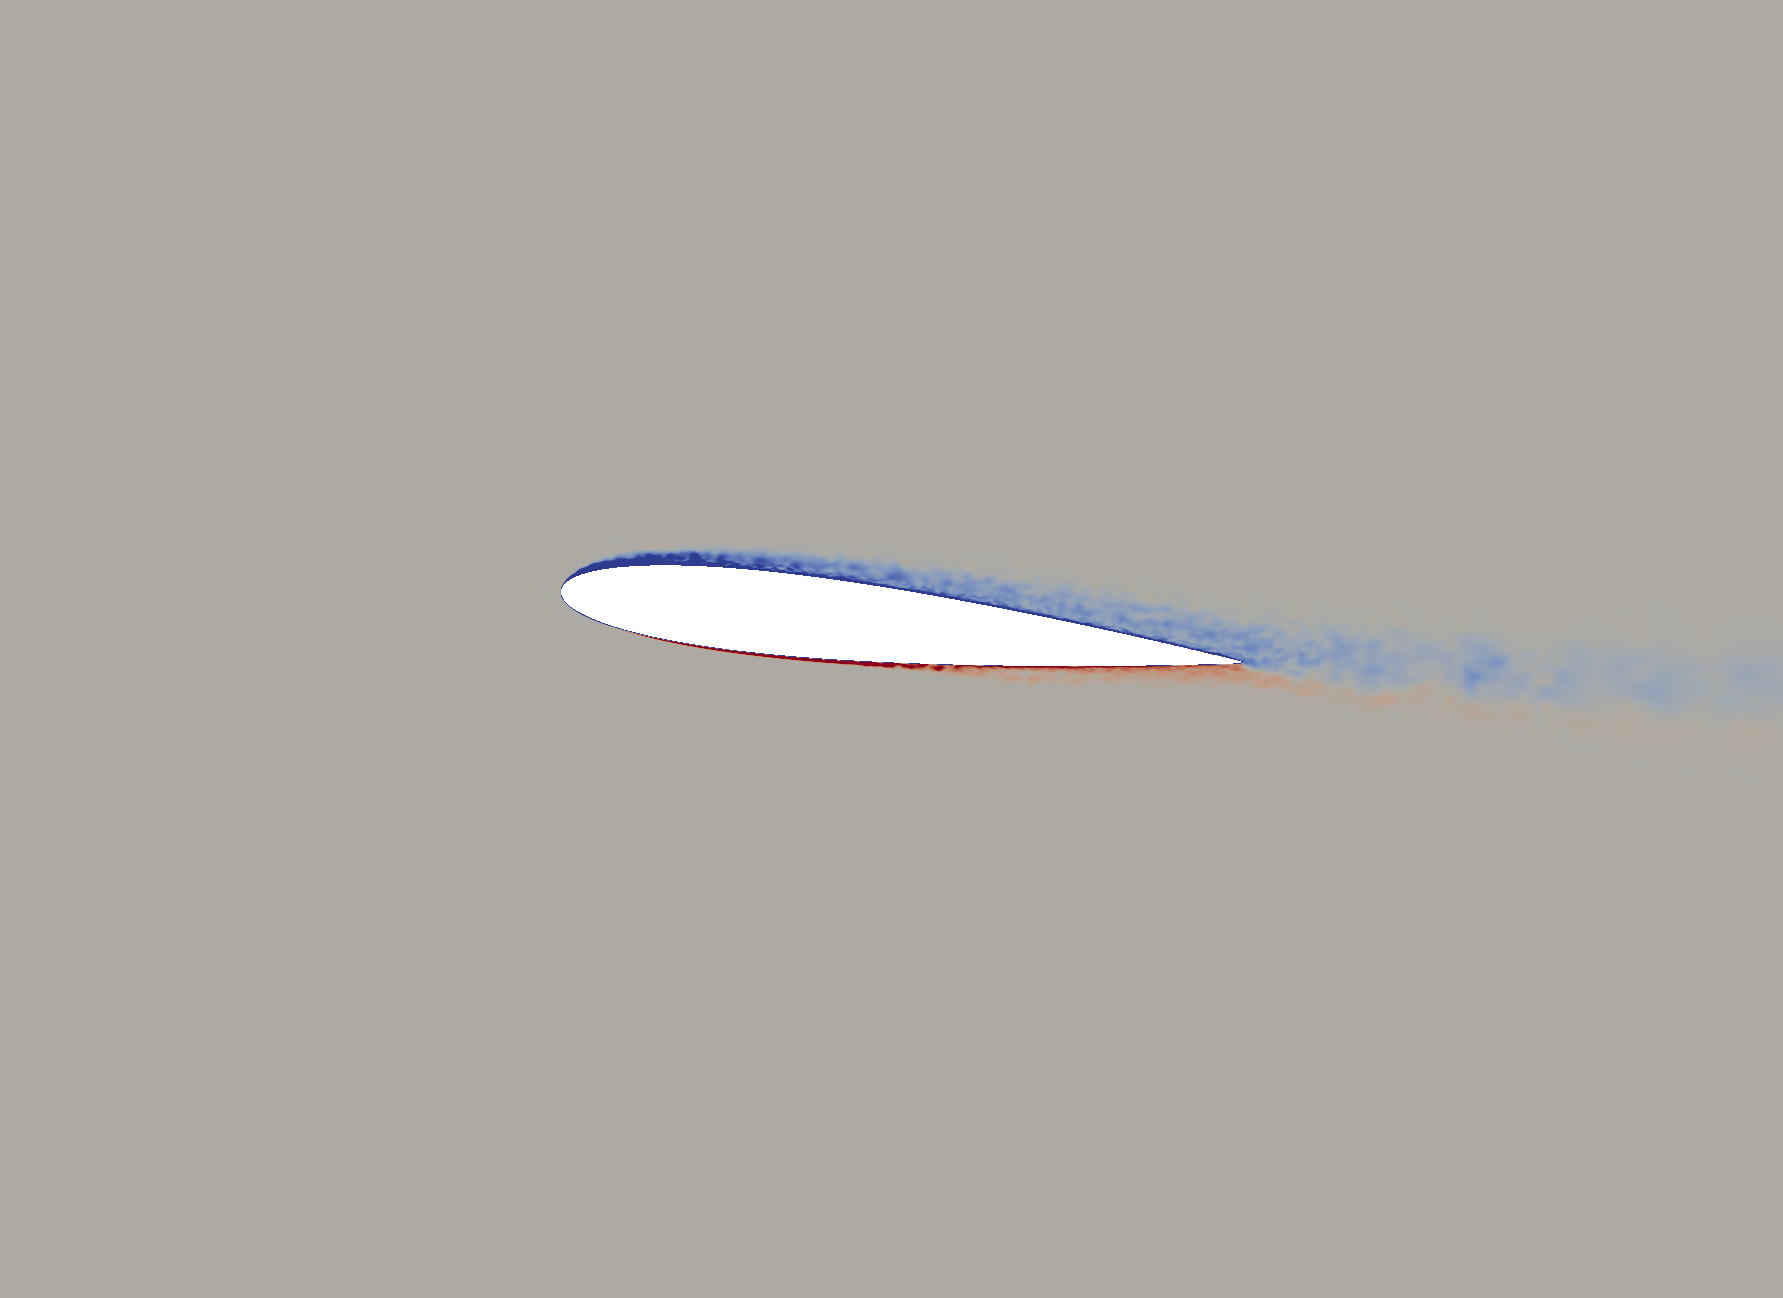
\includegraphics[width=1\textwidth]{figures/Vorticity_plots/Re_1m_1pt0/phase_240.png}
		\caption{$Re=1e6$, $\psi$ = $240^\circ$, $\tilde{t}=0.667$}
		\label{fig:Re_1m_1pt0_phi240}
	\end{subfigure}
	
	\begin{subfigure}[b]{0.32\textwidth}
		\centering
		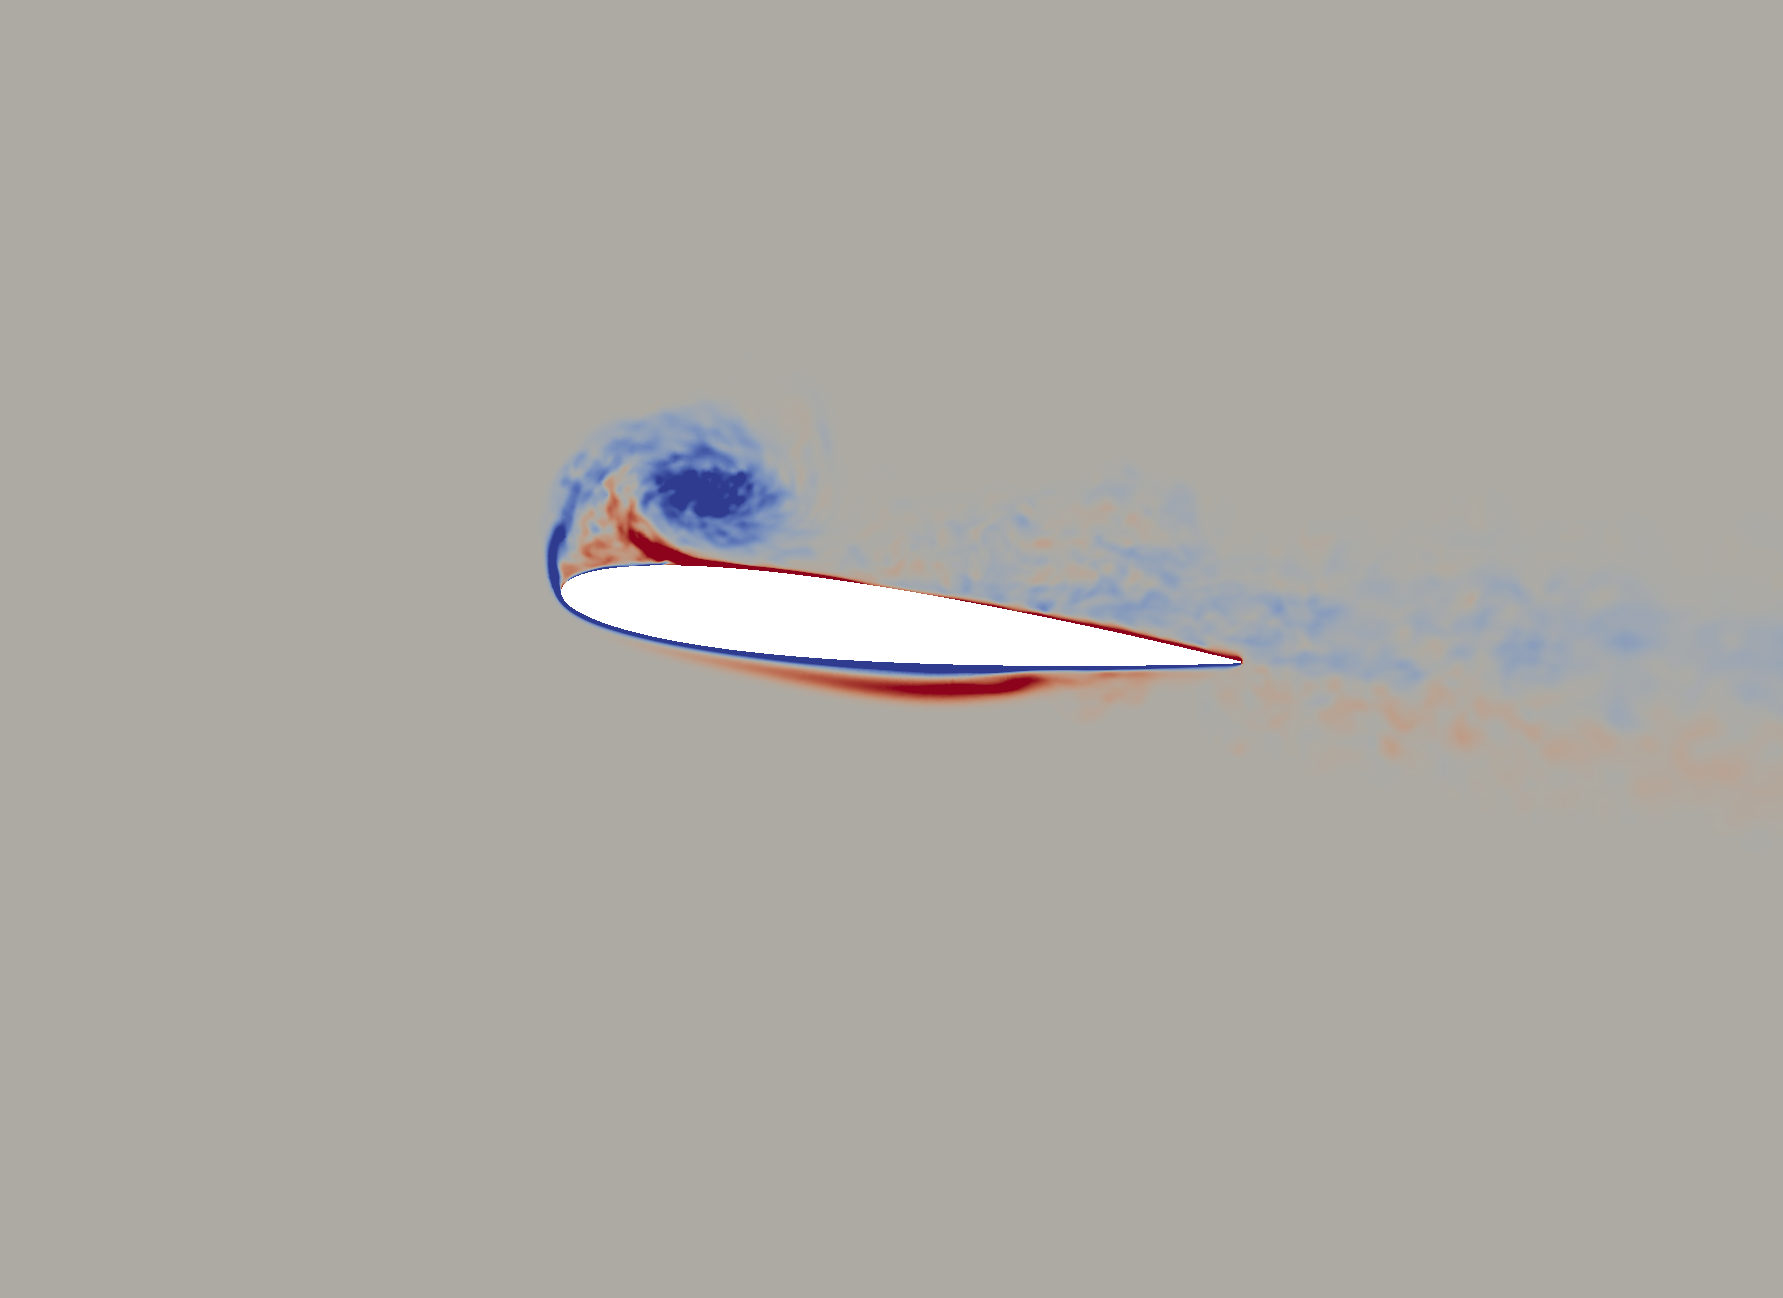
\includegraphics[width=1\textwidth]{figures/Vorticity_plots/Re_40k_1pt0/phase_255.png}
		\caption{$Re=4e4$, $\psi$ = $255^\circ$, $\tilde{t}=0.708$}
		\label{fig:Re_40k_1pt0_phi255}
	\end{subfigure}
	\begin{subfigure}[b]{0.32\textwidth}
		\centering
		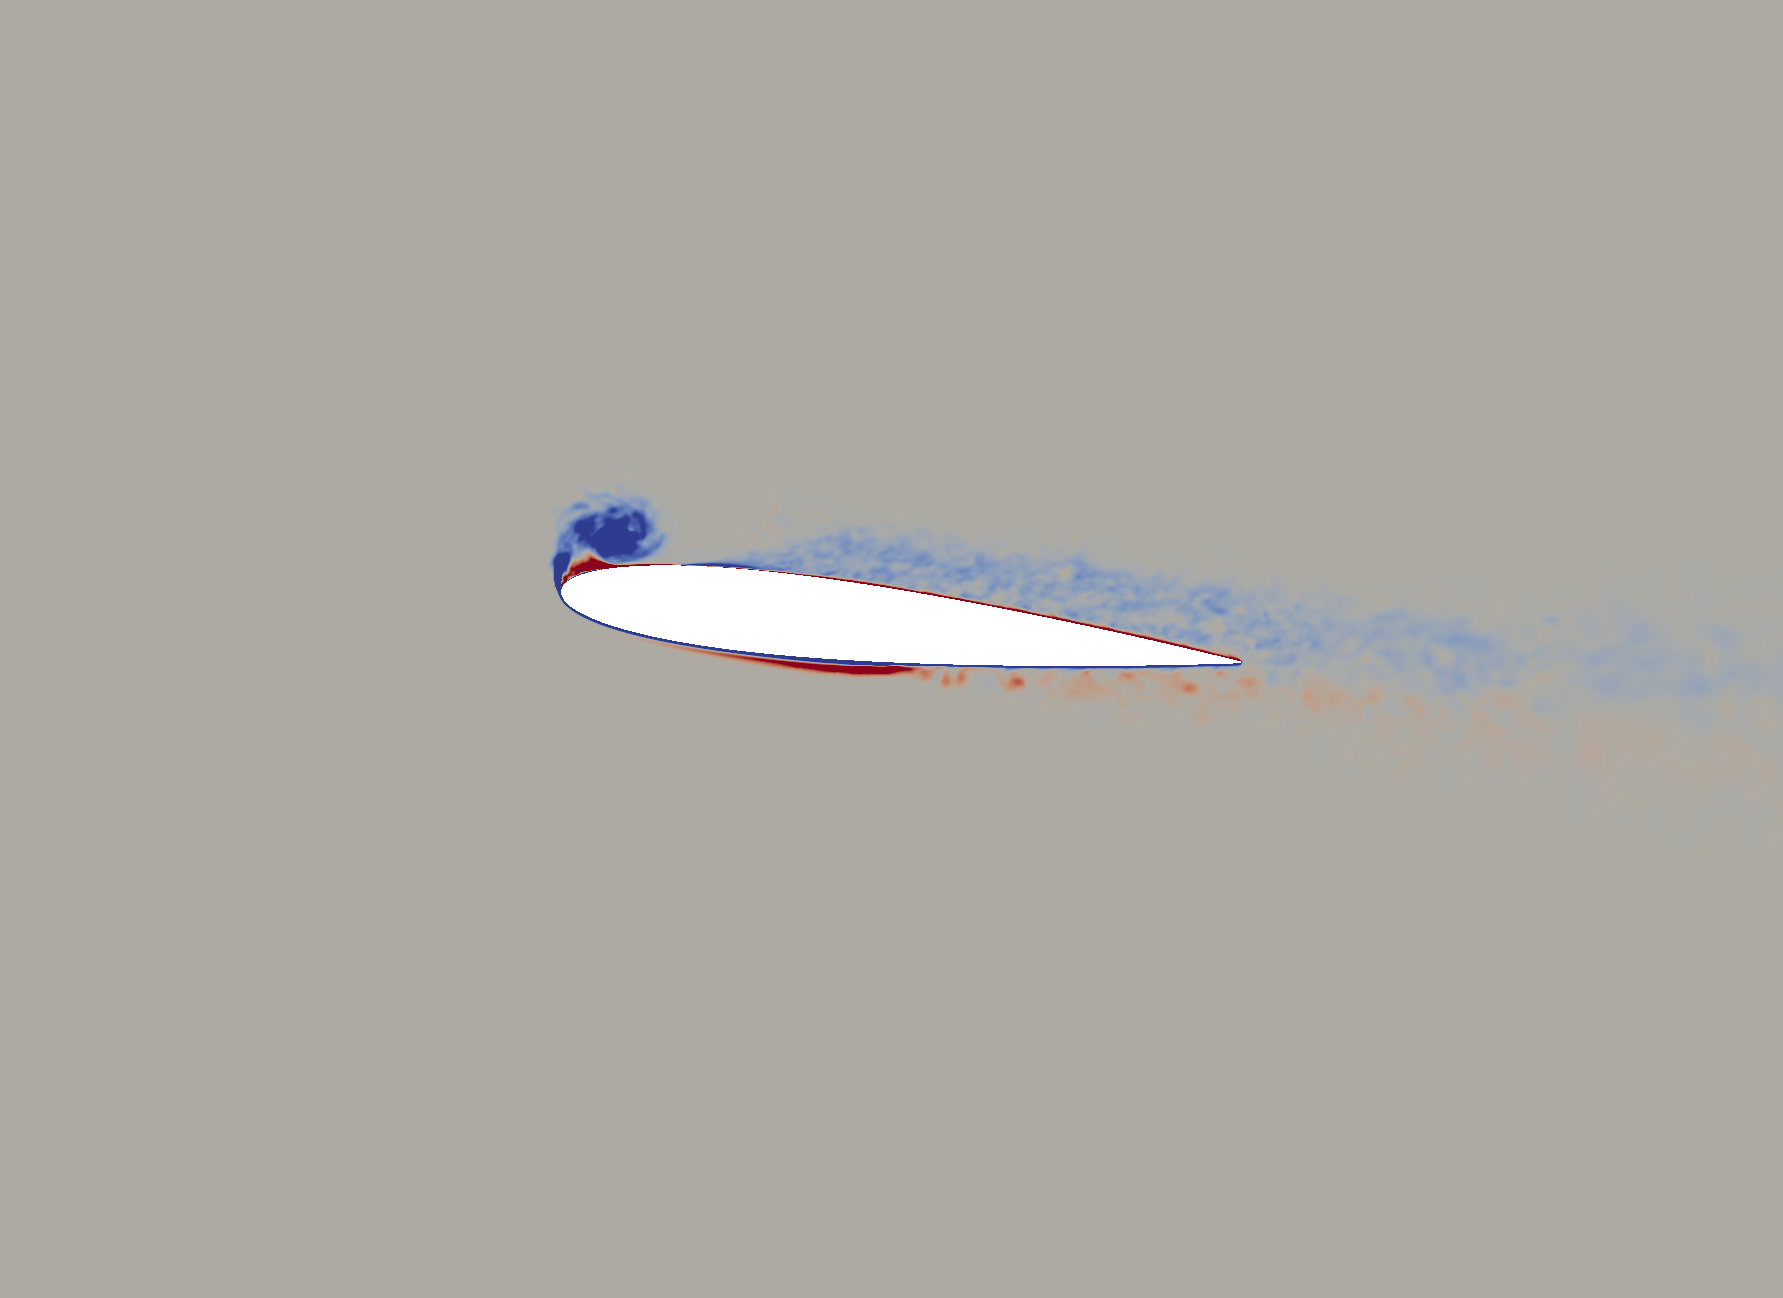
\includegraphics[width=1\textwidth]{figures/Vorticity_plots/Re_200k_1pt0/phase_255.png}
		\caption{$Re=2e5$, $\psi$ = $255^\circ$, $\tilde{t}=0.708$}
		\label{fig:Re_200k_1pt0_phi255}
	\end{subfigure}
	\begin{subfigure}[b]{0.32\textwidth}
		\centering
		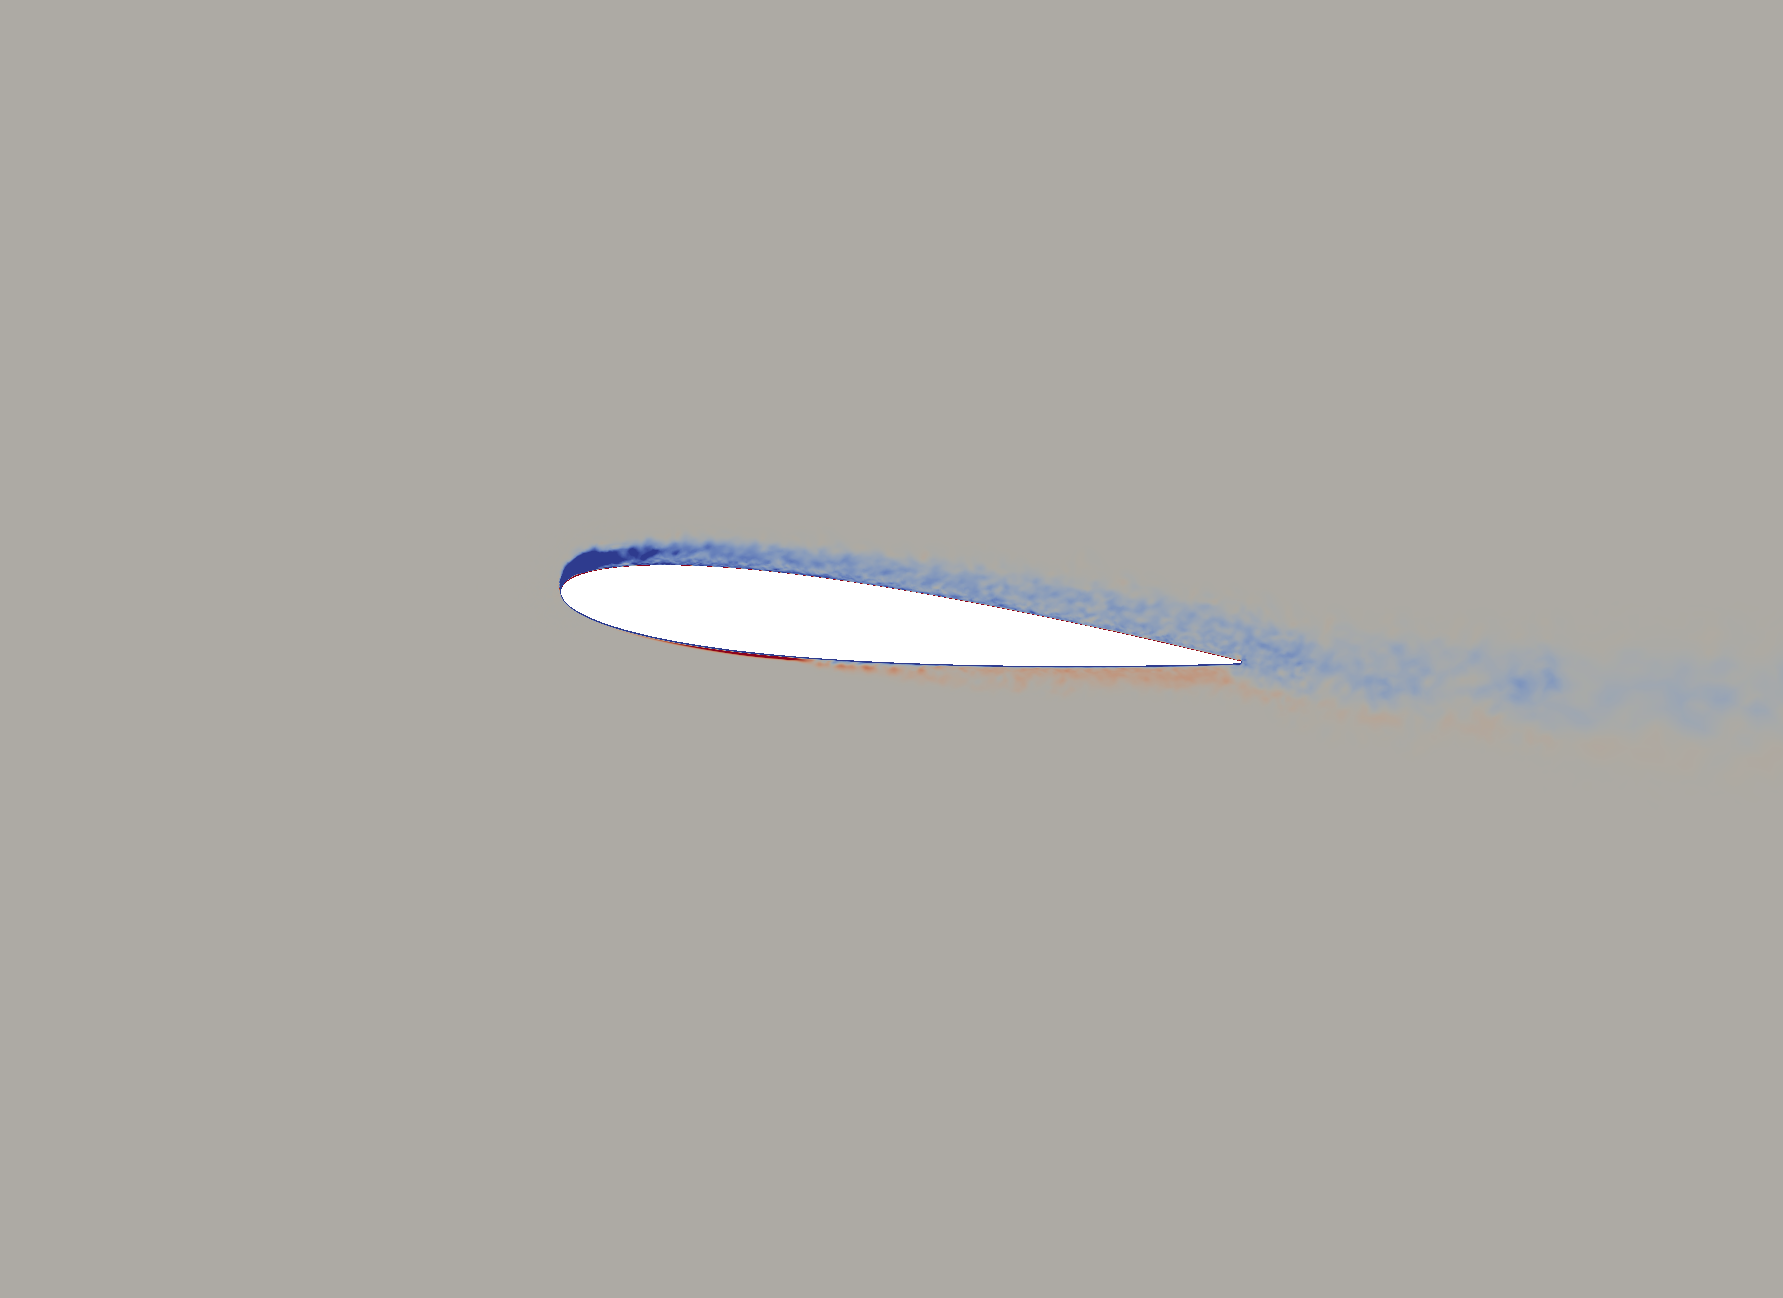
\includegraphics[width=1\textwidth]{figures/Vorticity_plots/Re_1m_1pt0/phase_255.png}
		\caption{$Re=1e6$, $\psi$ = $255^\circ$, $\tilde{t}=0.708$}
		\label{fig:Re_1m_1pt0_phi255}
	\end{subfigure}
	
	\caption{Spanwise vorticity at 8 different phases for $Re$=40,000 (left column), 200,000 (middle column) and 1,000,000 (right column) at $\mu_{sect}$ = 1.0}
	\label{fig:vortScreen_1pt0}
\end{figure}


\begin{figure}[H]\ContinuedFloat
	\centering
	\begin{subfigure}[b]{0.32\textwidth}
		\centering
		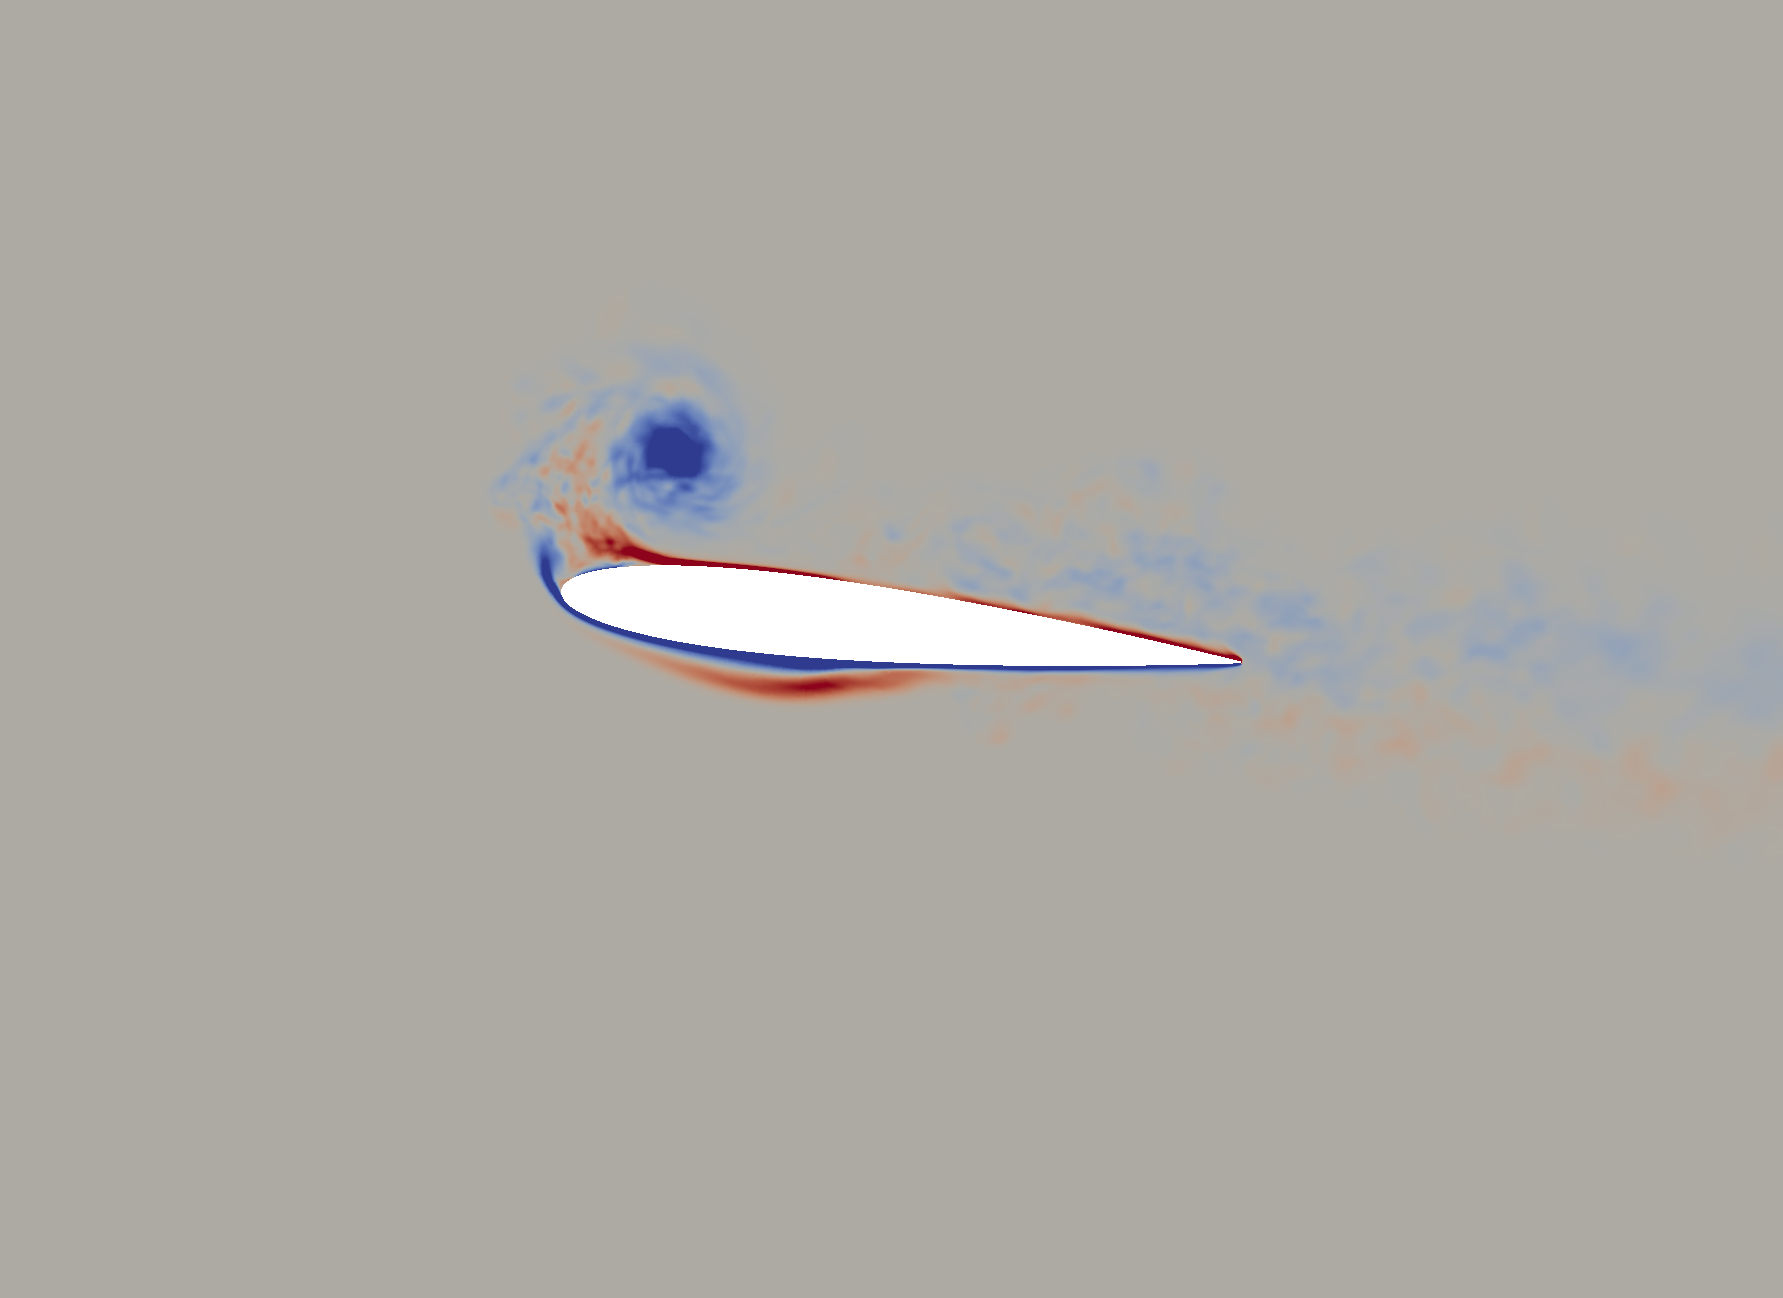
\includegraphics[width=1\textwidth]{figures/Vorticity_plots/Re_40k_1pt0/phase_270.png}
		\caption{$Re=4e4$, $\psi$ = $270^\circ$, $\tilde{t}=0.750$}
		\label{fig:Re_40k_1pt0_phi270}
	\end{subfigure}
	\begin{subfigure}[b]{0.32\textwidth}
		\centering
		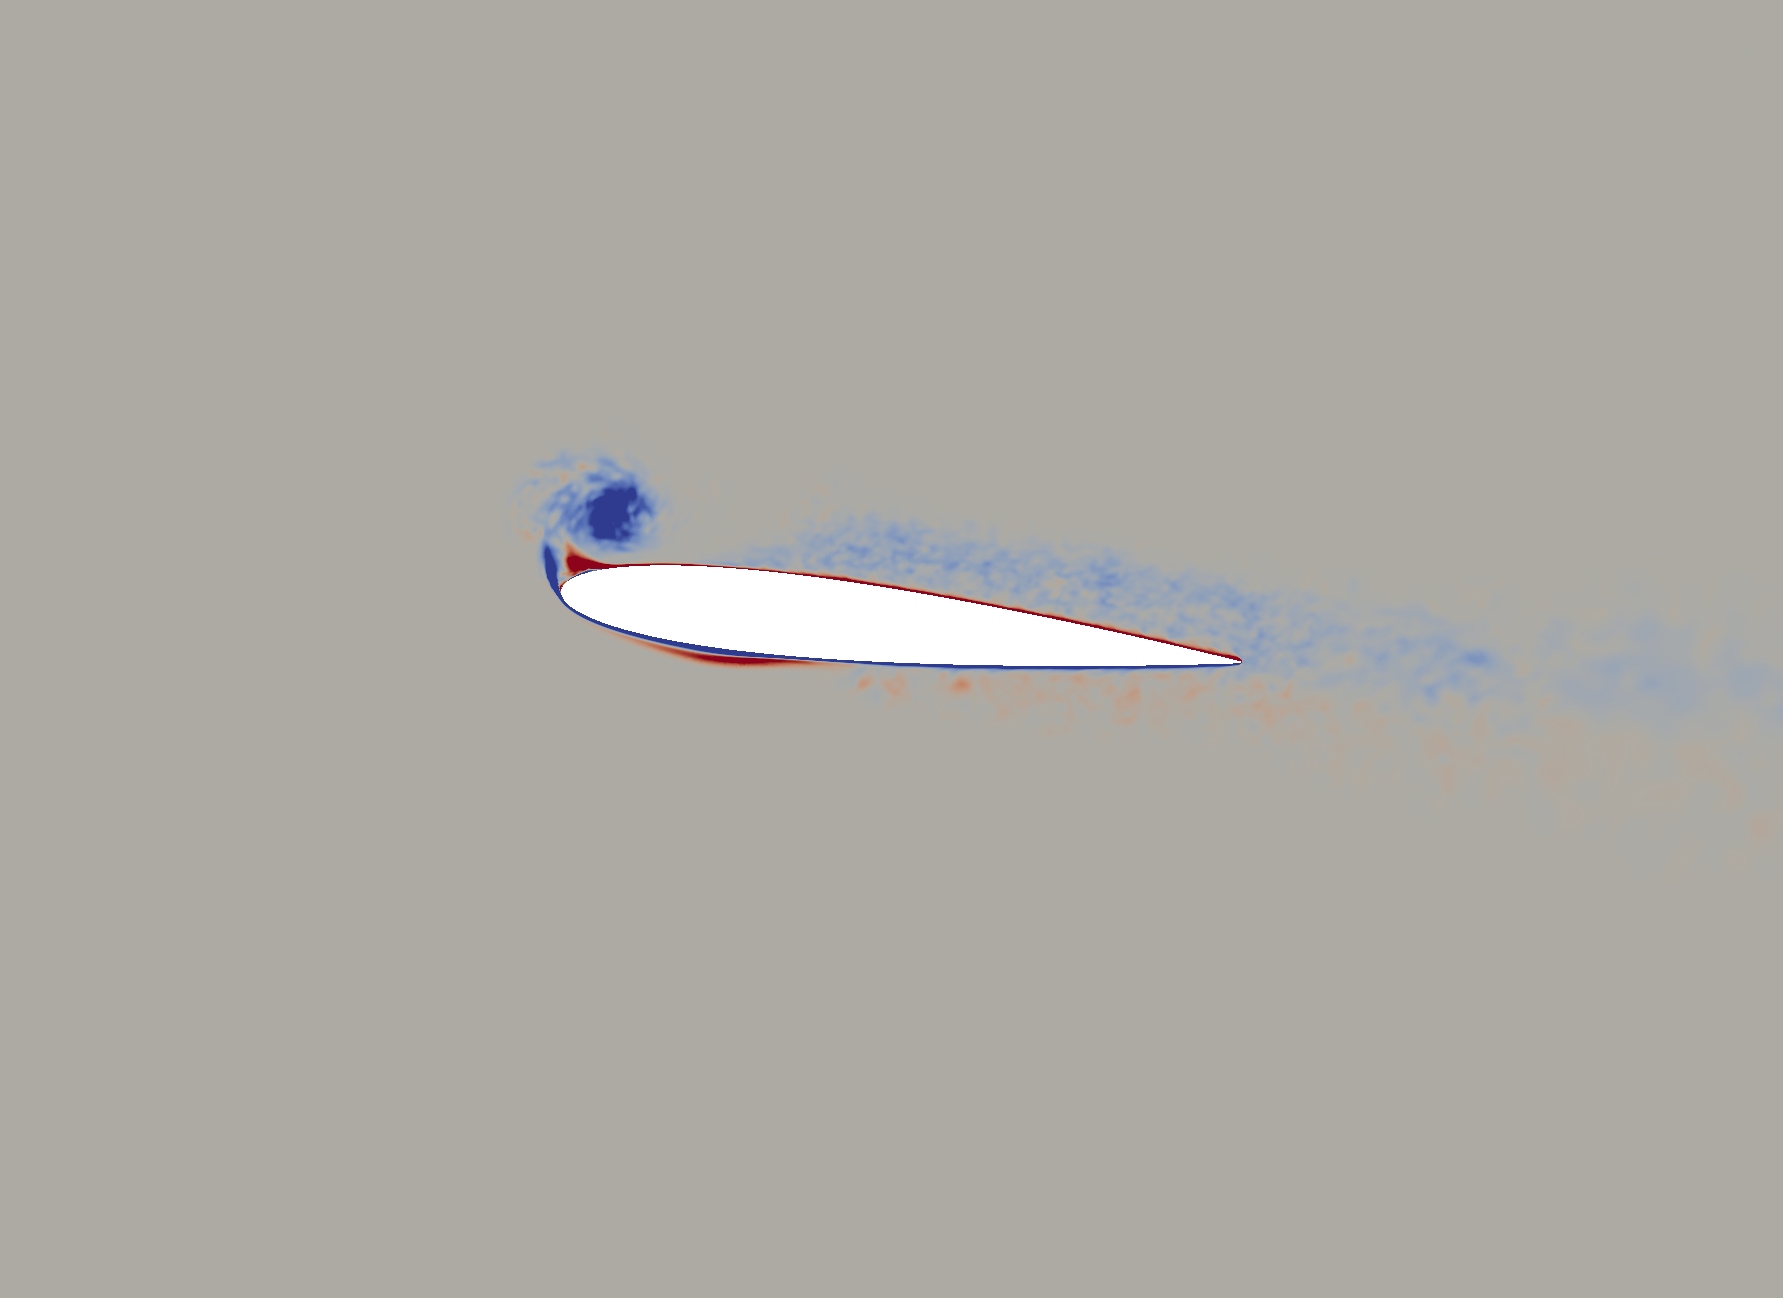
\includegraphics[width=1\textwidth]{figures/Vorticity_plots/Re_200k_1pt0/phase_270.png}
		\caption{$Re=2e5$, $\psi$ = $270^\circ$, $\tilde{t}=0.750$}
		\label{fig:Re_200k_1pt0_phi270}
	\end{subfigure}
	\begin{subfigure}[b]{0.32\textwidth}
		\centering
		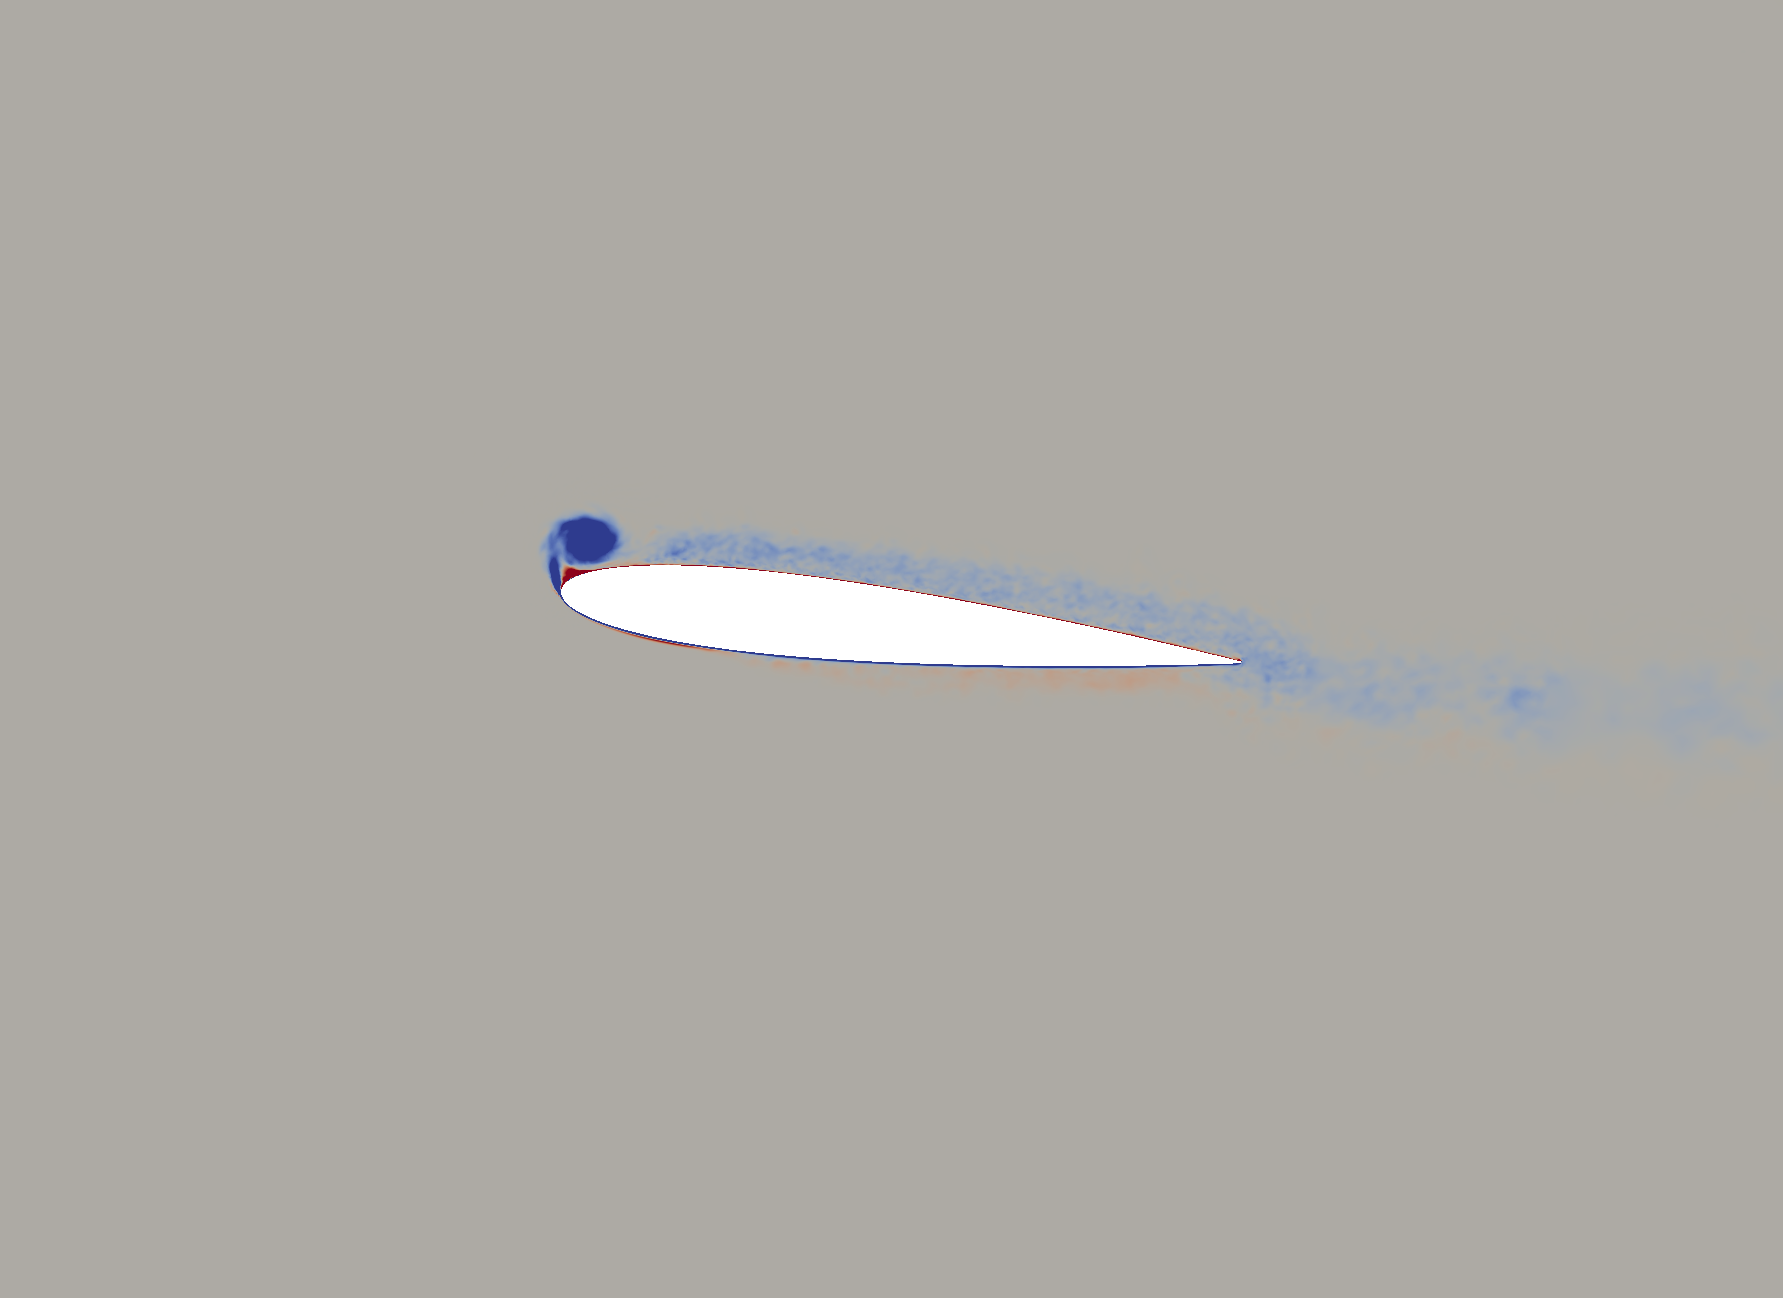
\includegraphics[width=1\textwidth]{figures/Vorticity_plots/Re_1m_1pt0/phase_270.png}
		\caption{$Re=1e6$, $\psi$ = $270^\circ$, $\tilde{t}=0.750$}
		\label{fig:Re_1m_1pt0_phi270}
	\end{subfigure}
	
	\begin{subfigure}[b]{0.32\textwidth}
		\centering
		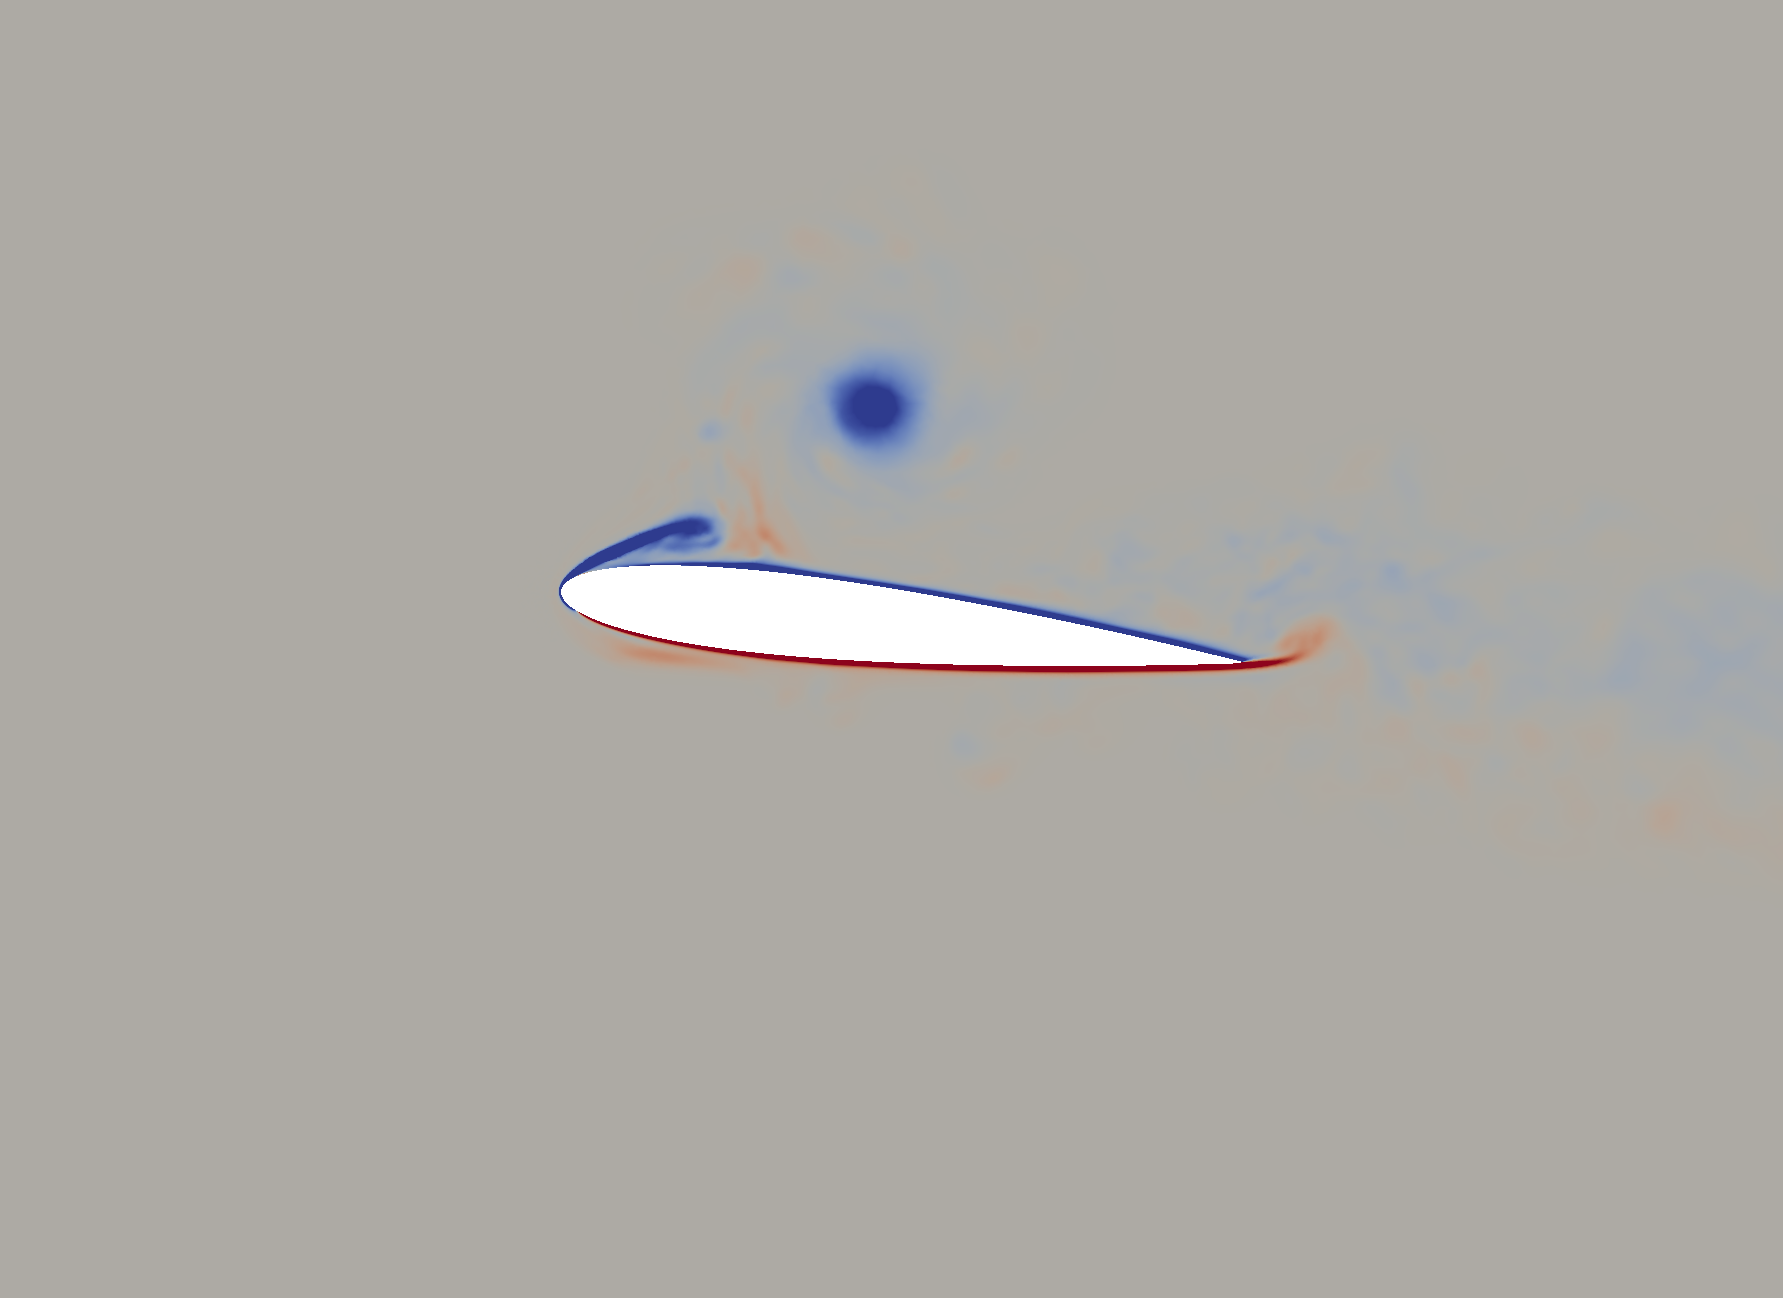
\includegraphics[width=1\textwidth]{figures/Vorticity_plots/Re_40k_1pt0/phase_315.png}
		\caption{$Re=4e4$, $\psi$ = $315^\circ$, $\tilde{t}=0.875$}
		\label{fig:Re_40k_1pt0_phi315}
	\end{subfigure}
	\begin{subfigure}[b]{0.32\textwidth}
		\centering
		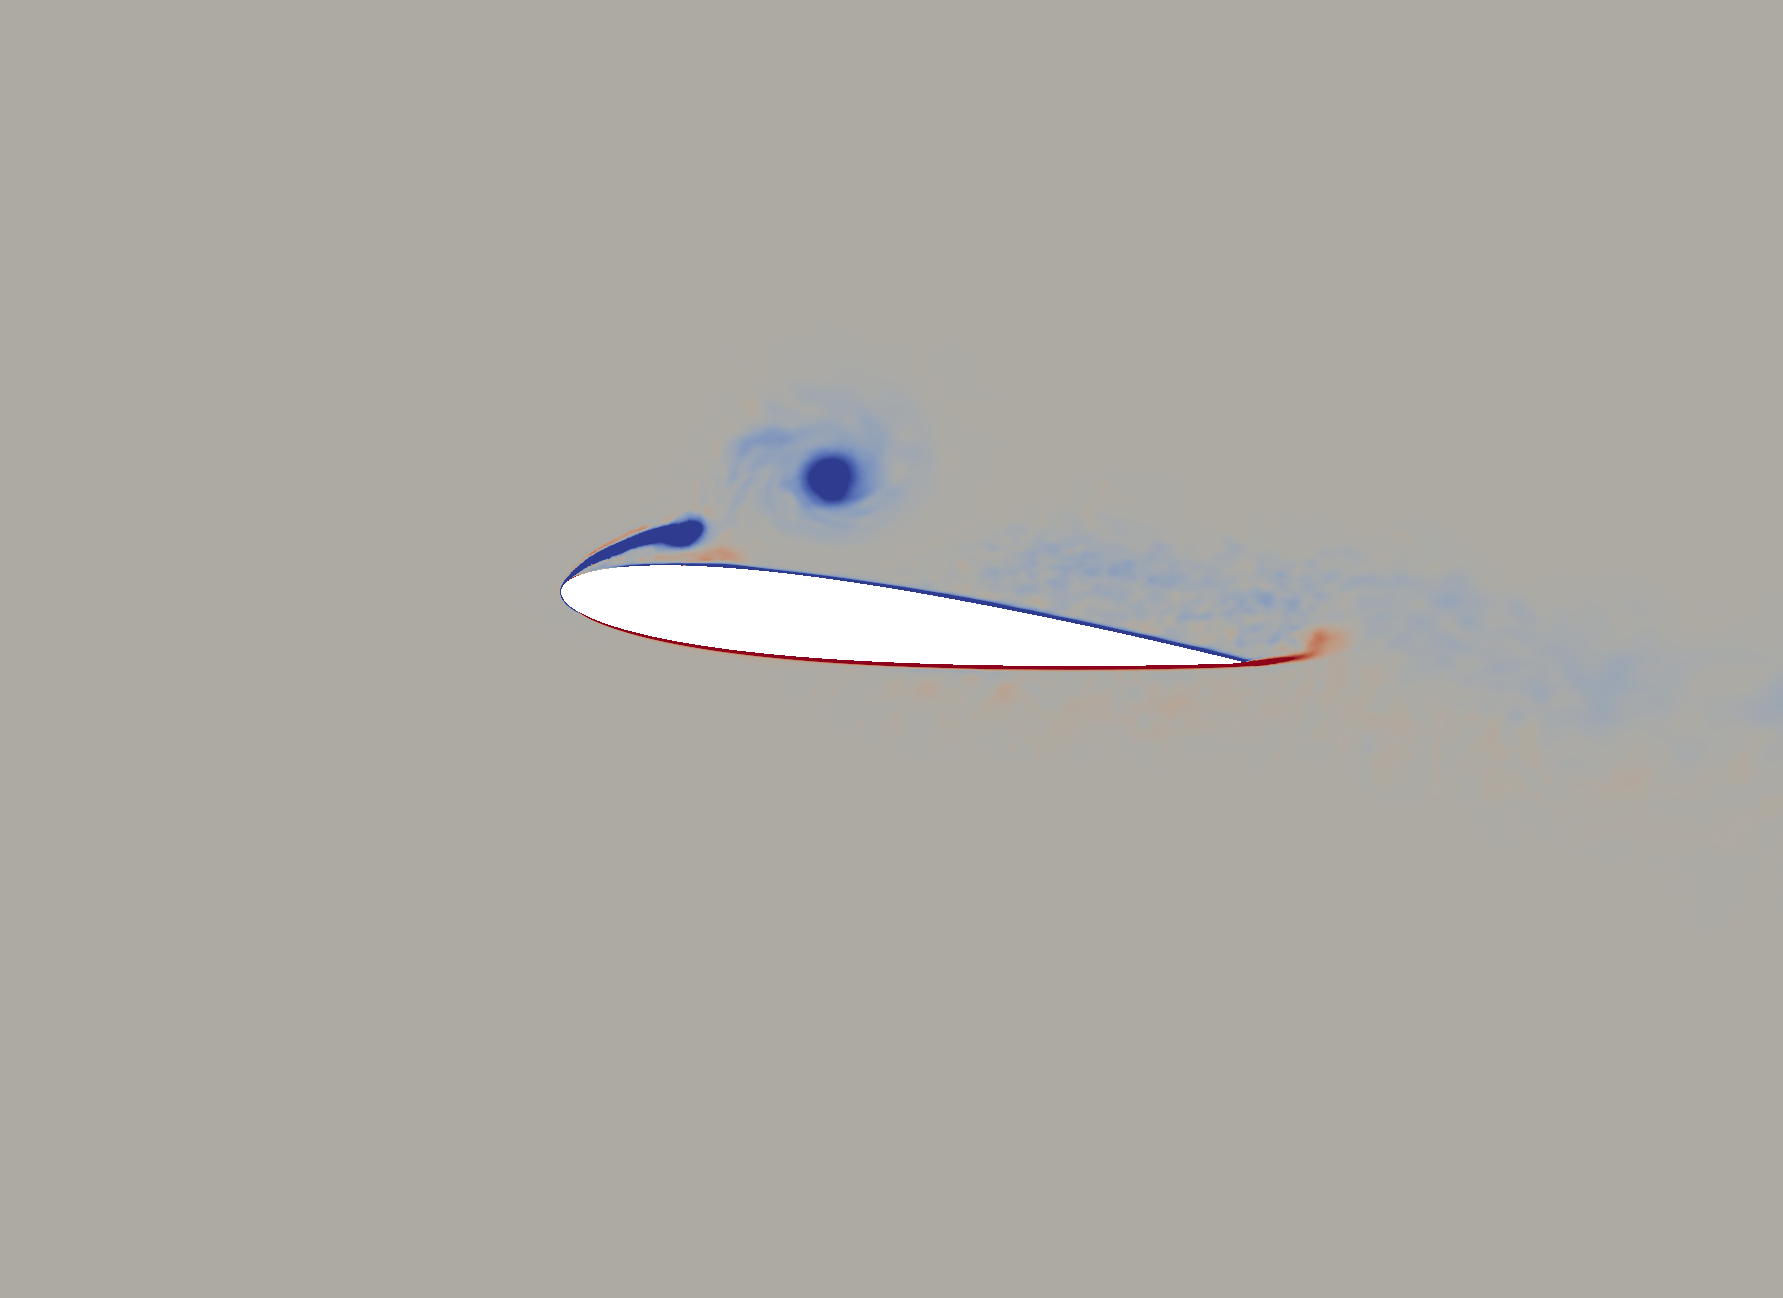
\includegraphics[width=1\textwidth]{figures/Vorticity_plots/Re_200k_1pt0/phase_315.png}
		\caption{$Re=2e5$, $\psi$ = $315^\circ$, $\tilde{t}=0.875$}
		\label{fig:Re_200k_1pt0_phi315}
	\end{subfigure}
	\begin{subfigure}[b]{0.32\textwidth}
		\centering
		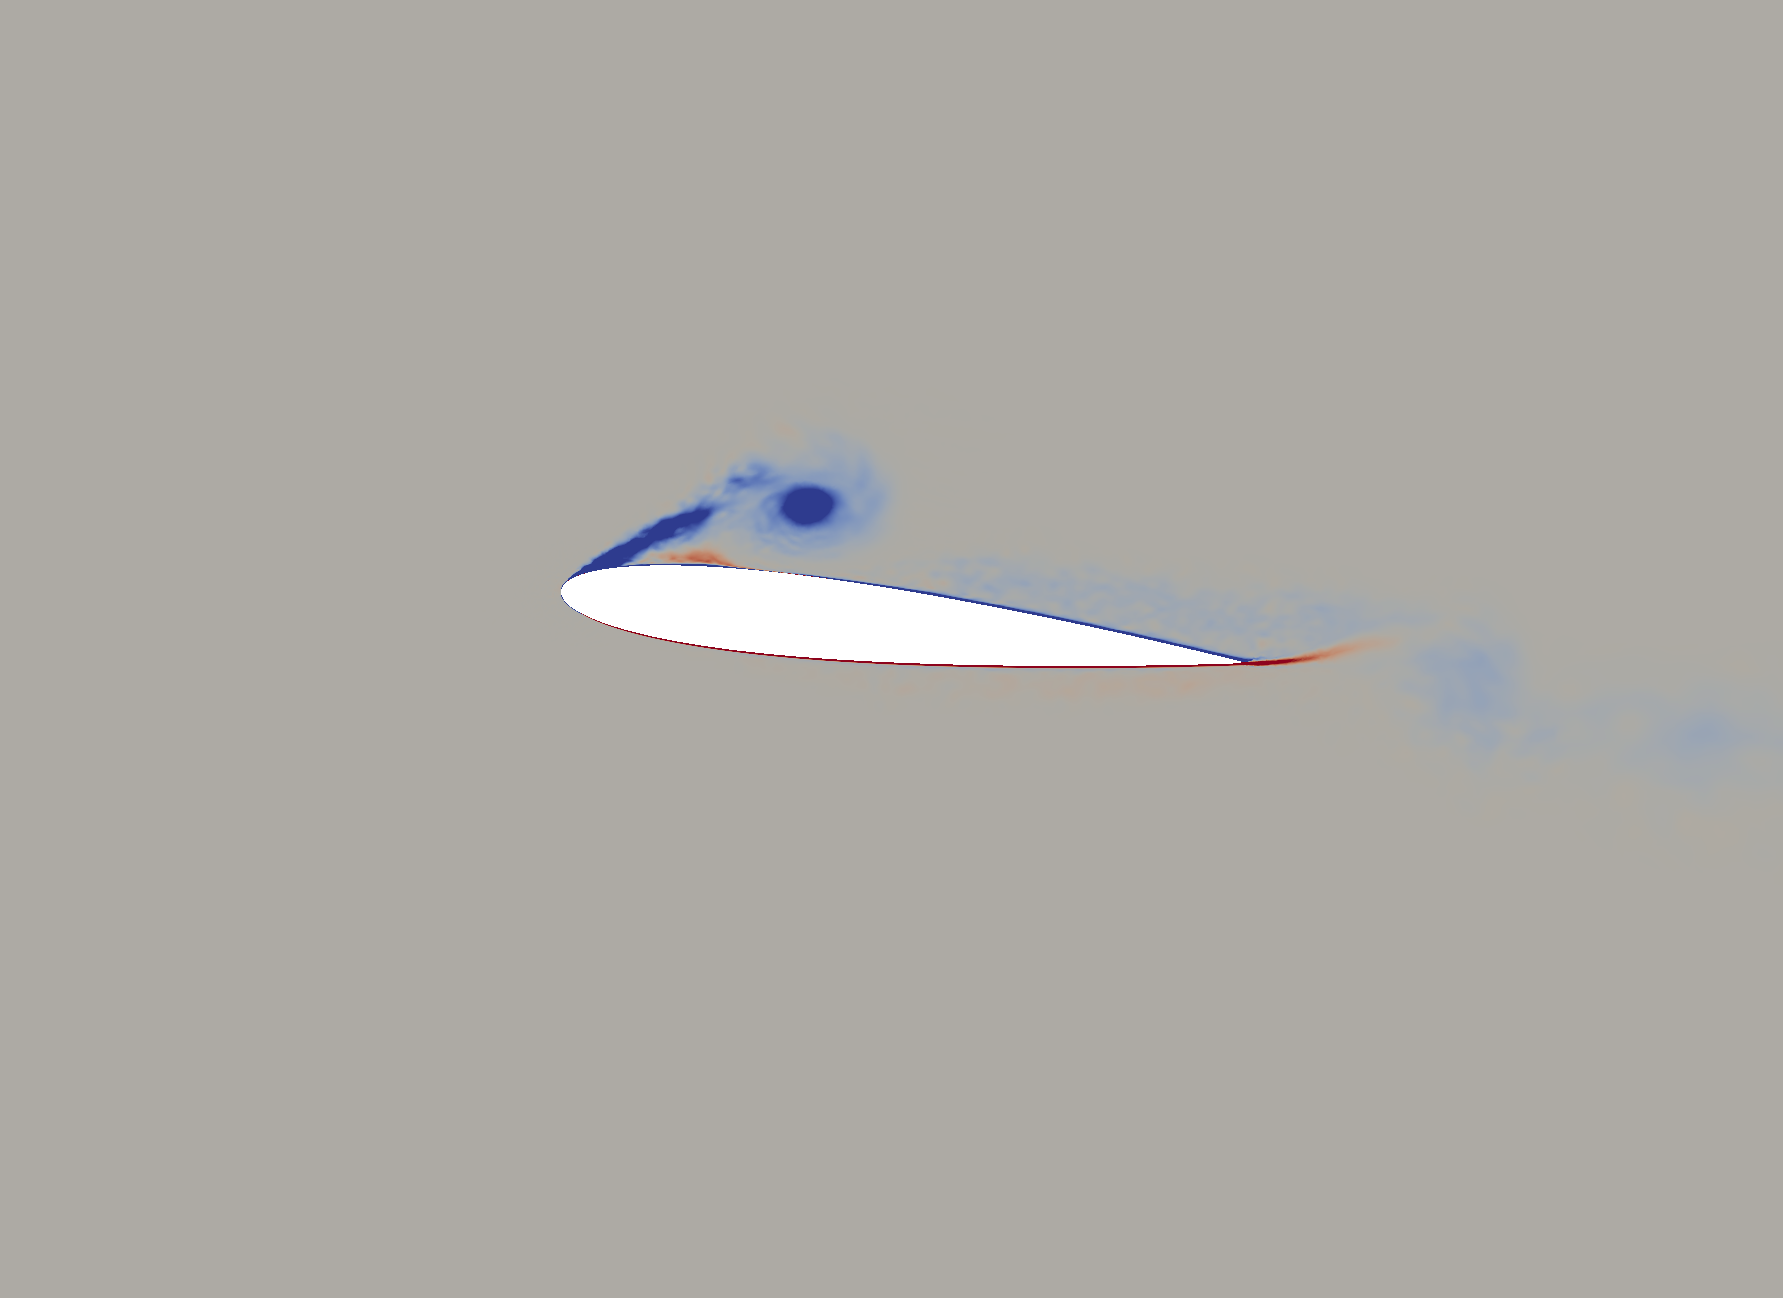
\includegraphics[width=1\textwidth]{figures/Vorticity_plots/Re_1m_1pt0/phase_315.png}
		\caption{$Re=1e6$, $\psi$ = $315^\circ$, $\tilde{t}=0.875$}
		\label{fig:Re_1m_1pt0_phi315}
	\end{subfigure}
	
	\begin{subfigure}[b]{0.32\textwidth}
		\centering
		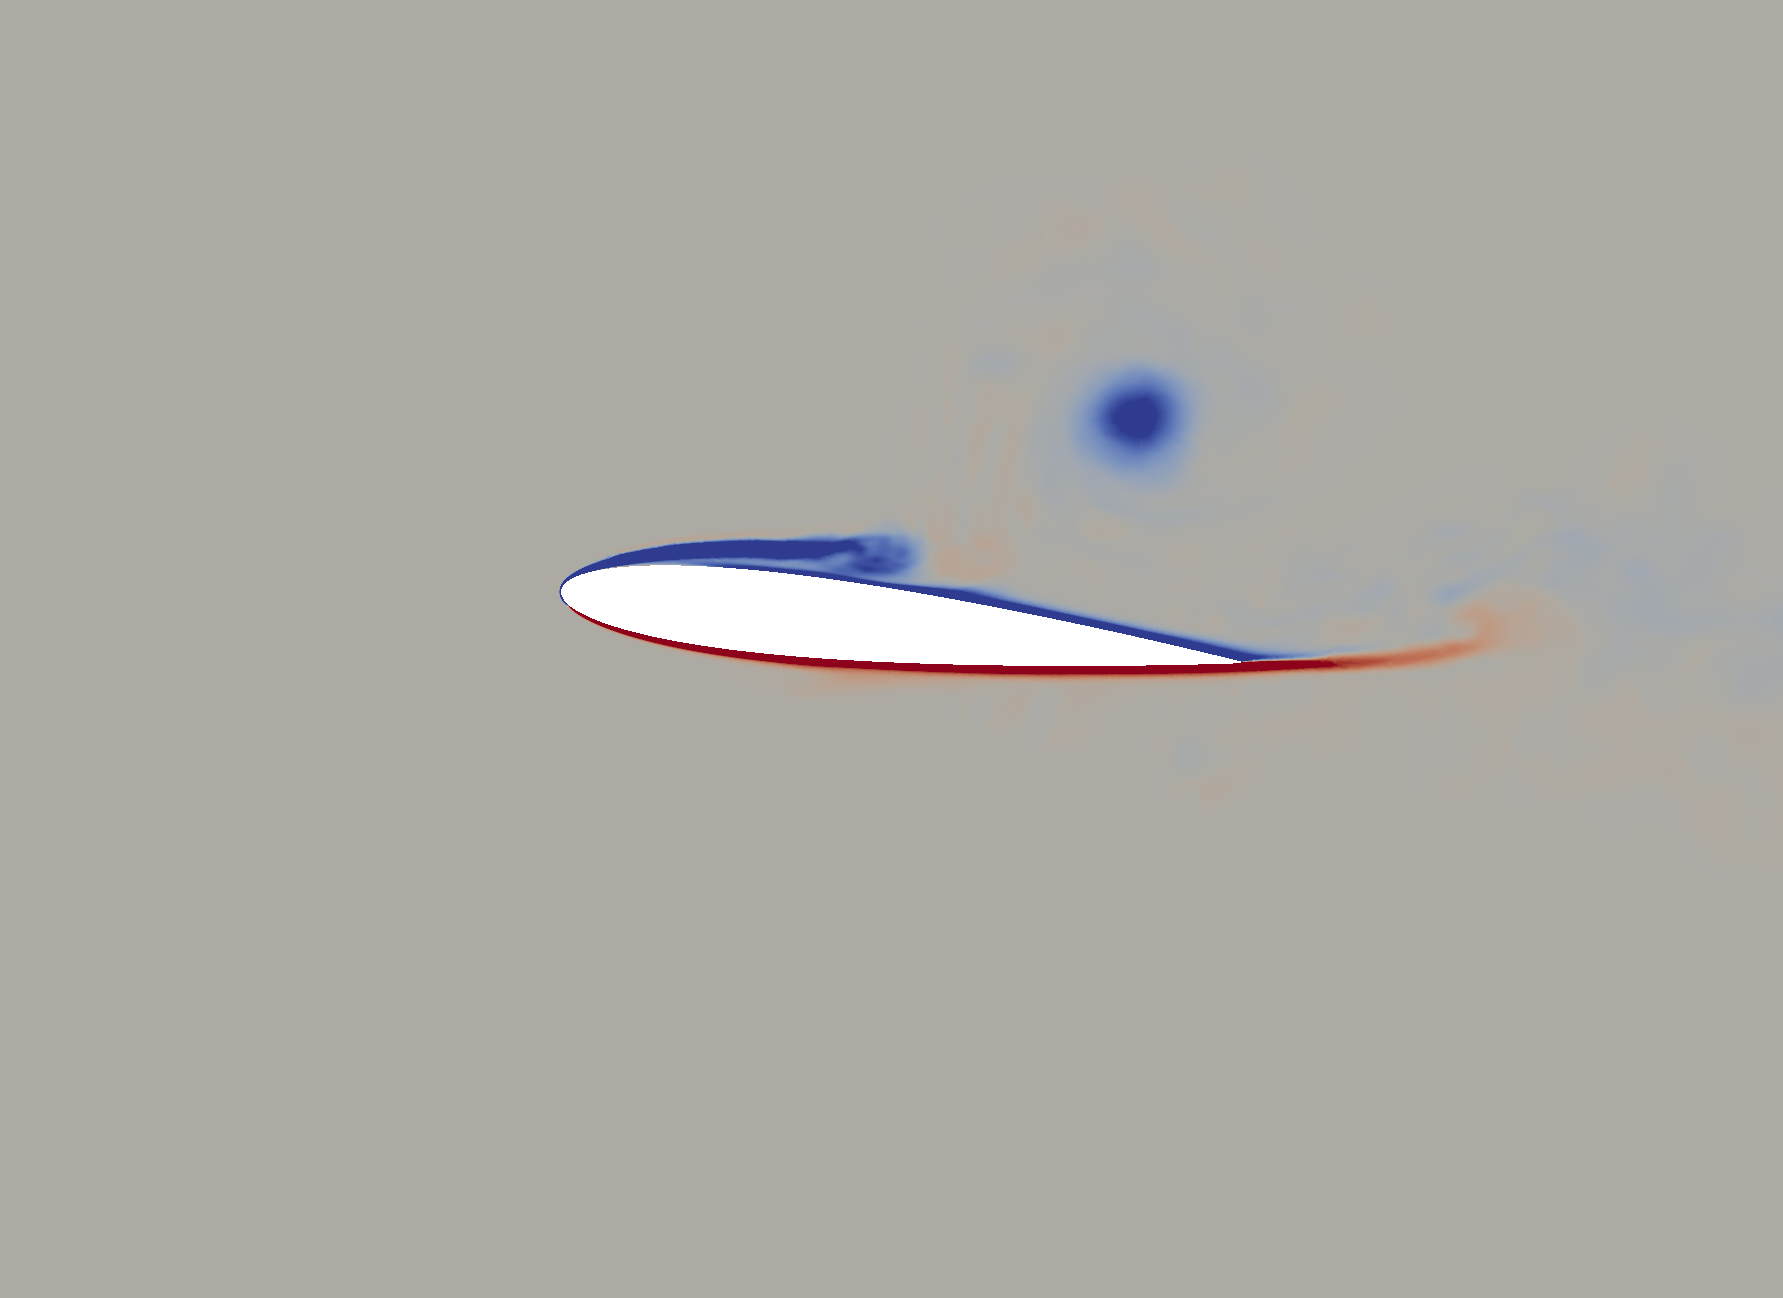
\includegraphics[width=1\textwidth]{figures/Vorticity_plots/Re_40k_1pt0/phase_330.png}
		\caption{$Re=4e4$, $\psi$ = $330^\circ$, $\tilde{t}=0.917$}
		\label{fig:Re_40k_1pt0_phi330}
	\end{subfigure}
	\begin{subfigure}[b]{0.32\textwidth}
		\centering
		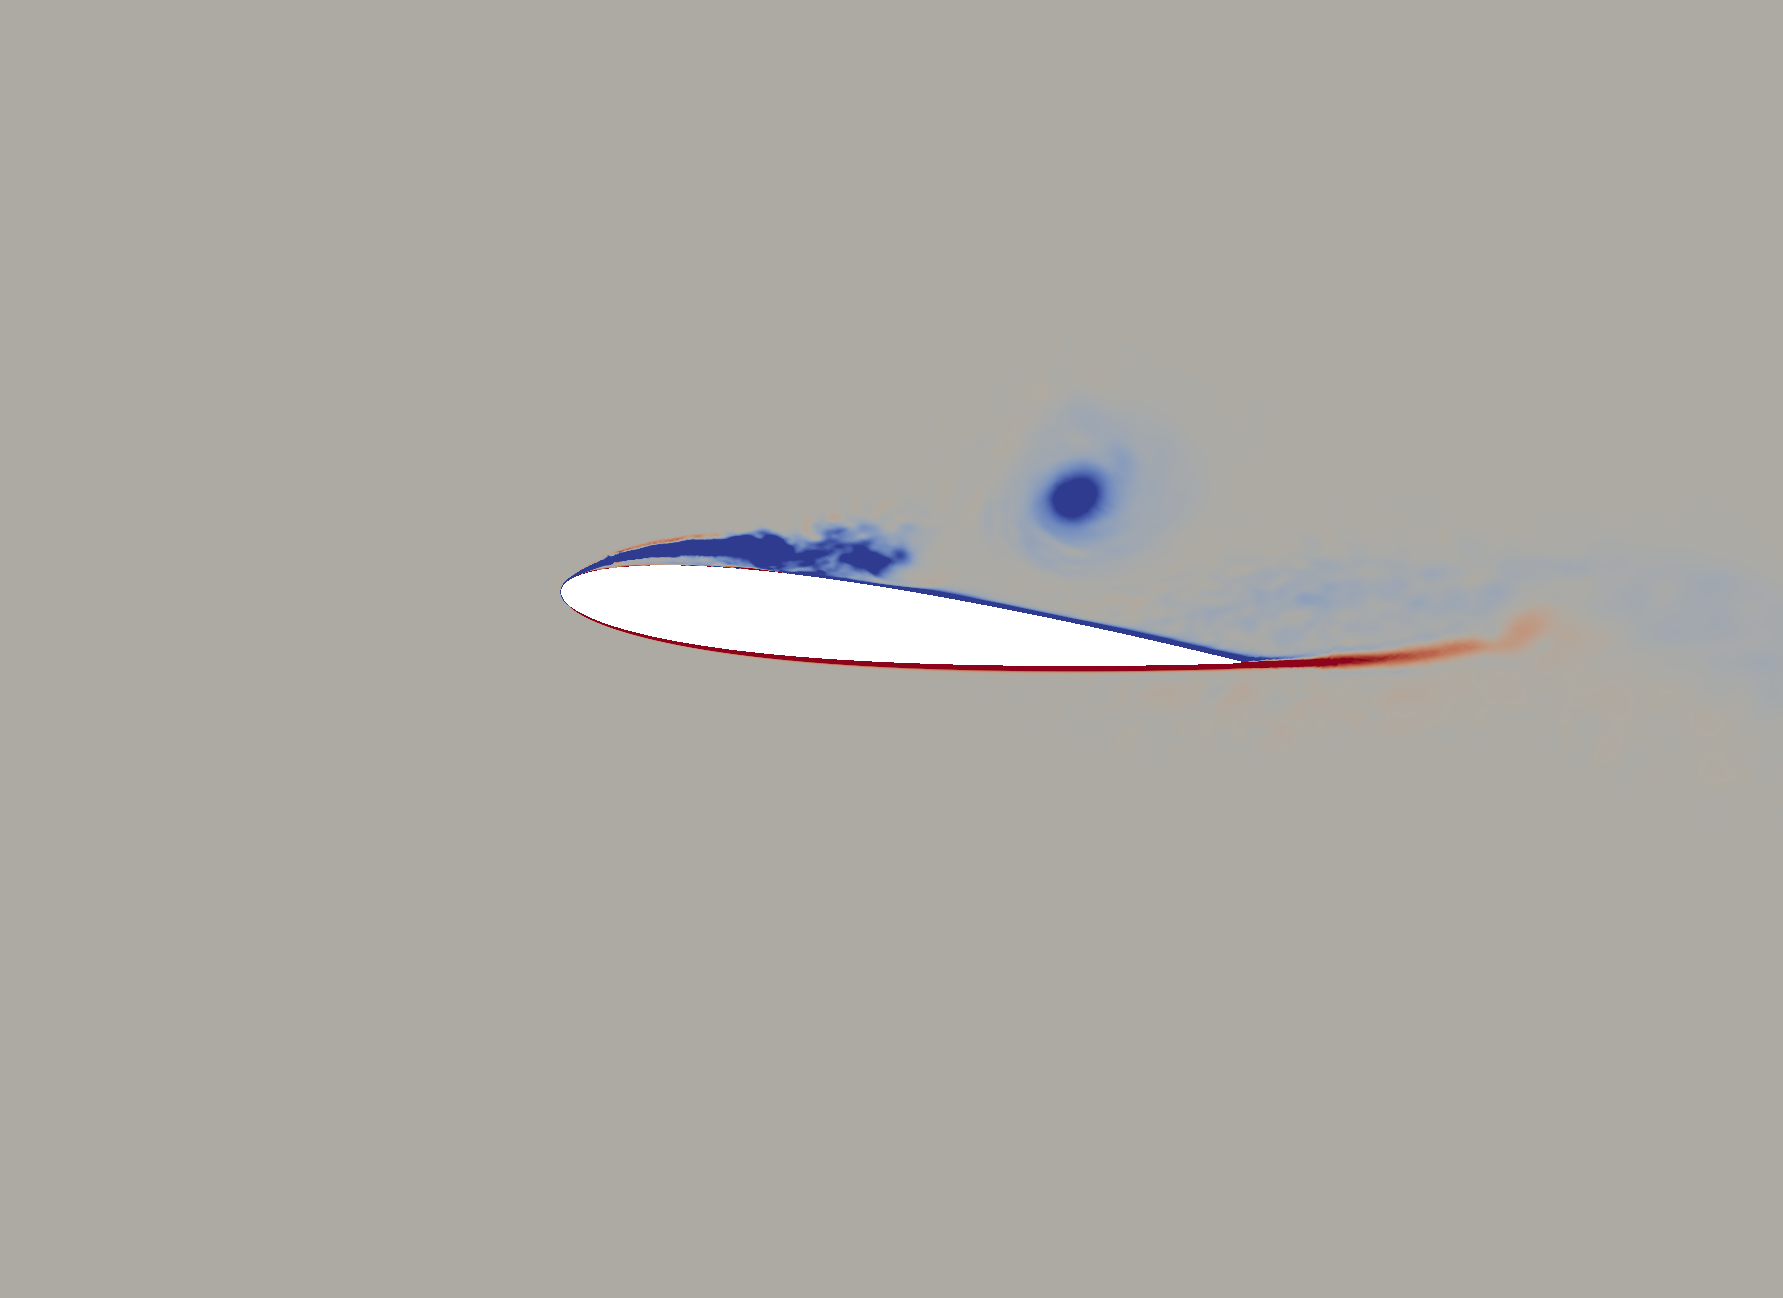
\includegraphics[width=1\textwidth]{figures/Vorticity_plots/Re_200k_1pt0/phase_330.png}
		\caption{$Re=2e5$, $\psi$ = $330^\circ$, $\tilde{t}=0.917$}
		\label{fig:Re_200k_1pt0_phi330}
	\end{subfigure}
	\begin{subfigure}[b]{0.32\textwidth}
		\centering
		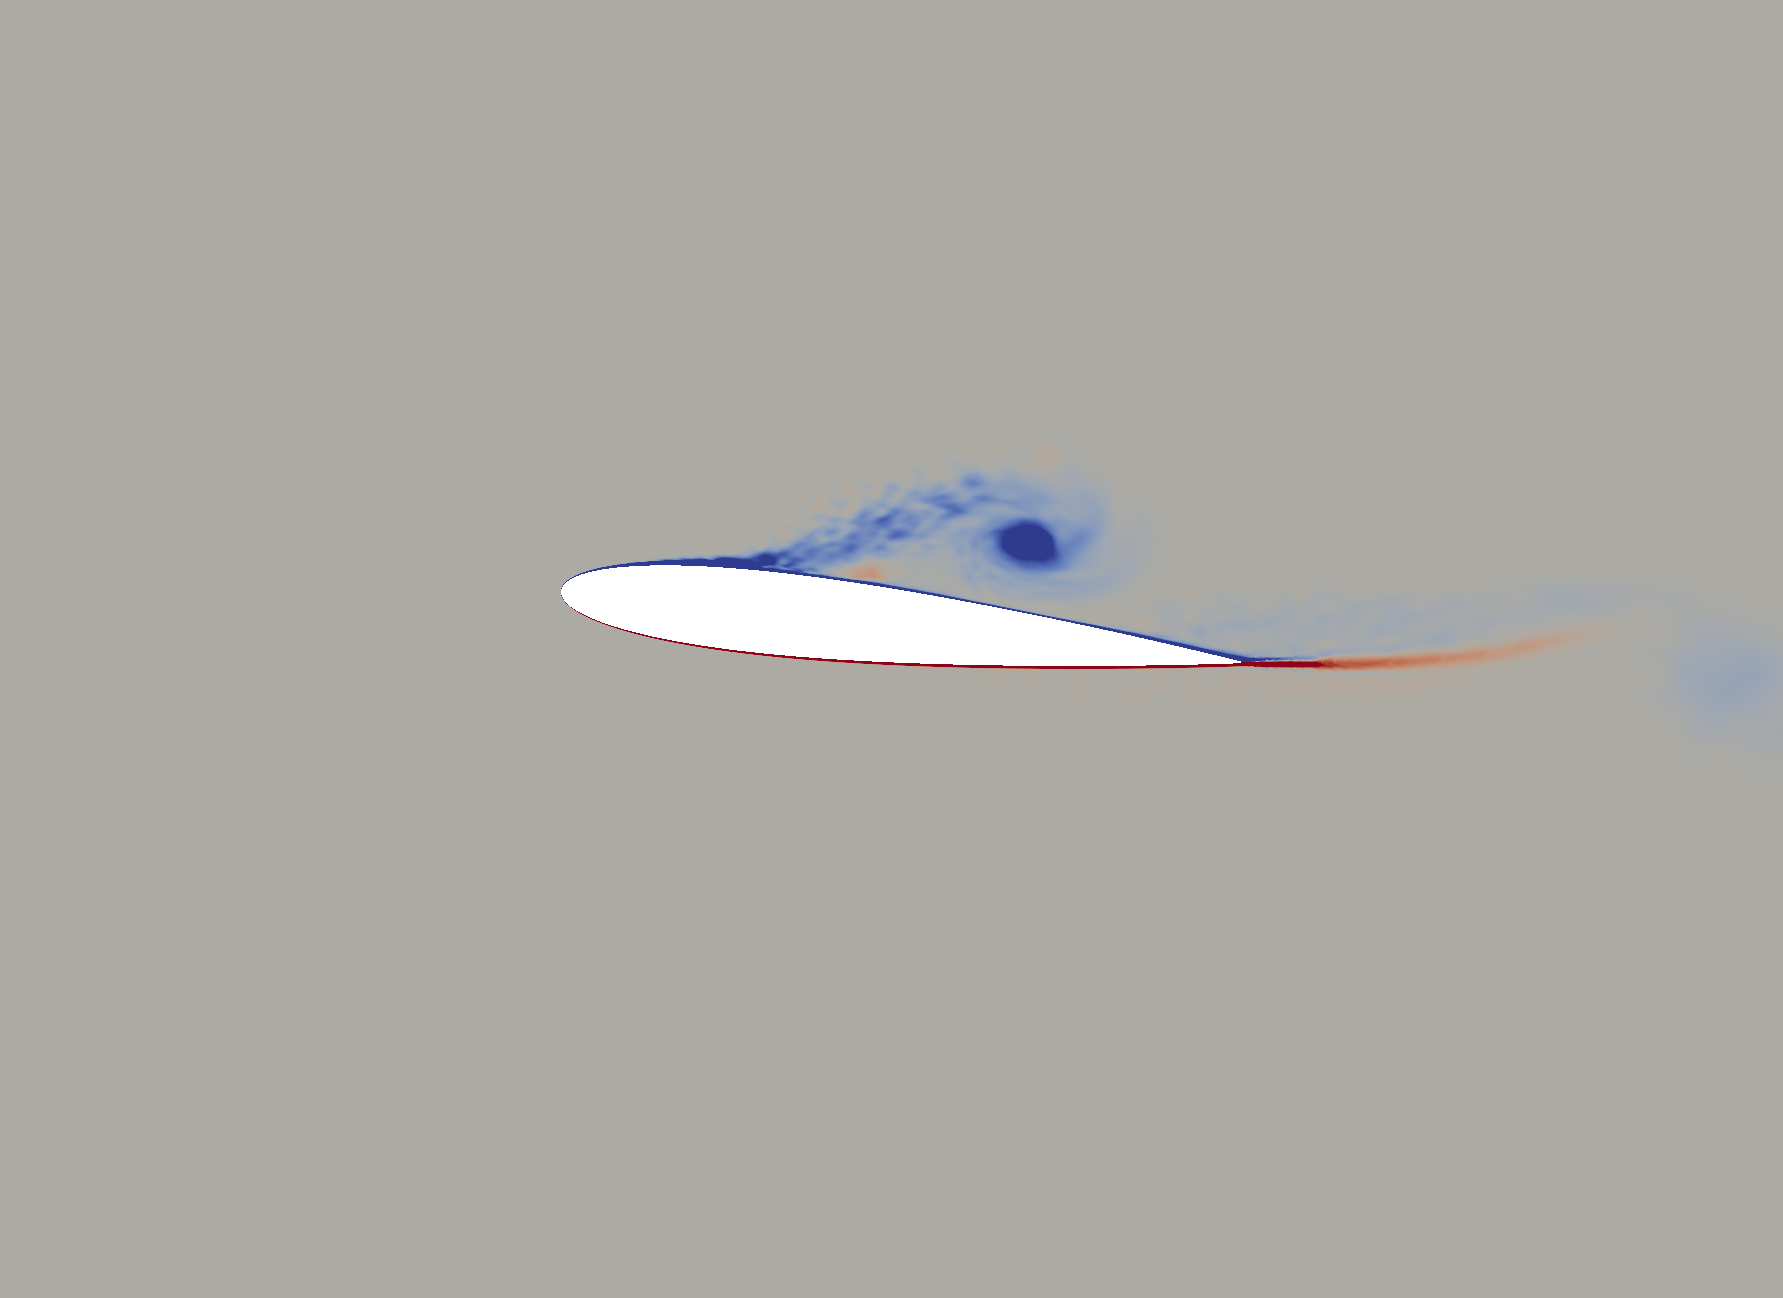
\includegraphics[width=1\textwidth]{figures/Vorticity_plots/Re_1m_1pt0/phase_330.png}
		\caption{$Re=1e6$,$\psi$ = $330^\circ$, $\tilde{t}=0.917$}
		\label{fig:Re_1m_1pt0_phi330}
	\end{subfigure}
	
	\begin{subfigure}[b]{0.32\textwidth}
		\centering
		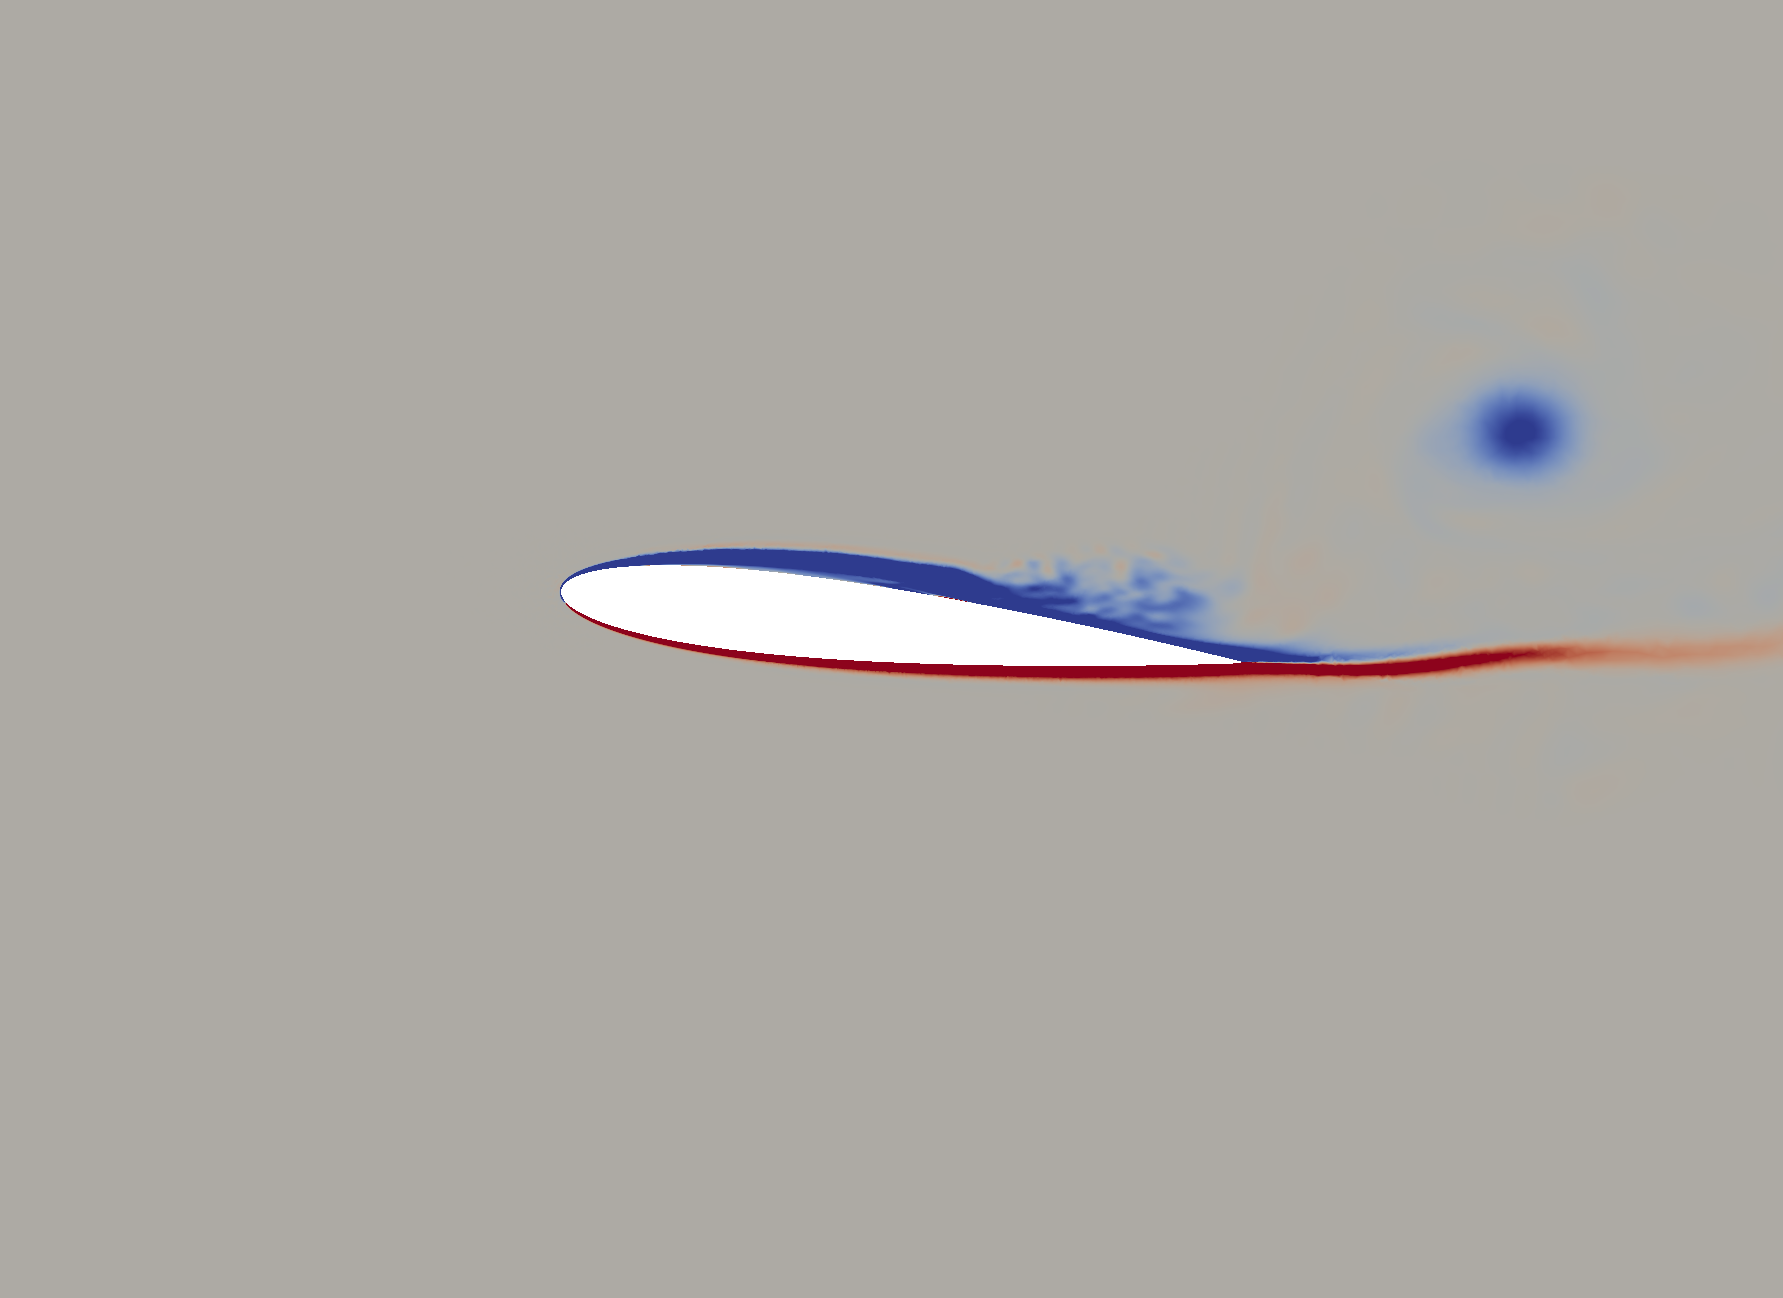
\includegraphics[width=1\textwidth]{figures/Vorticity_plots/Re_40k_1pt0/phase_345.png}
		\caption{$Re=4e4$, $\psi$ = $345^\circ$, $\tilde{t}=0.958$}
		\label{fig:Re_40k_1pt0_phi345}
	\end{subfigure}
	\begin{subfigure}[b]{0.32\textwidth}
		\centering
		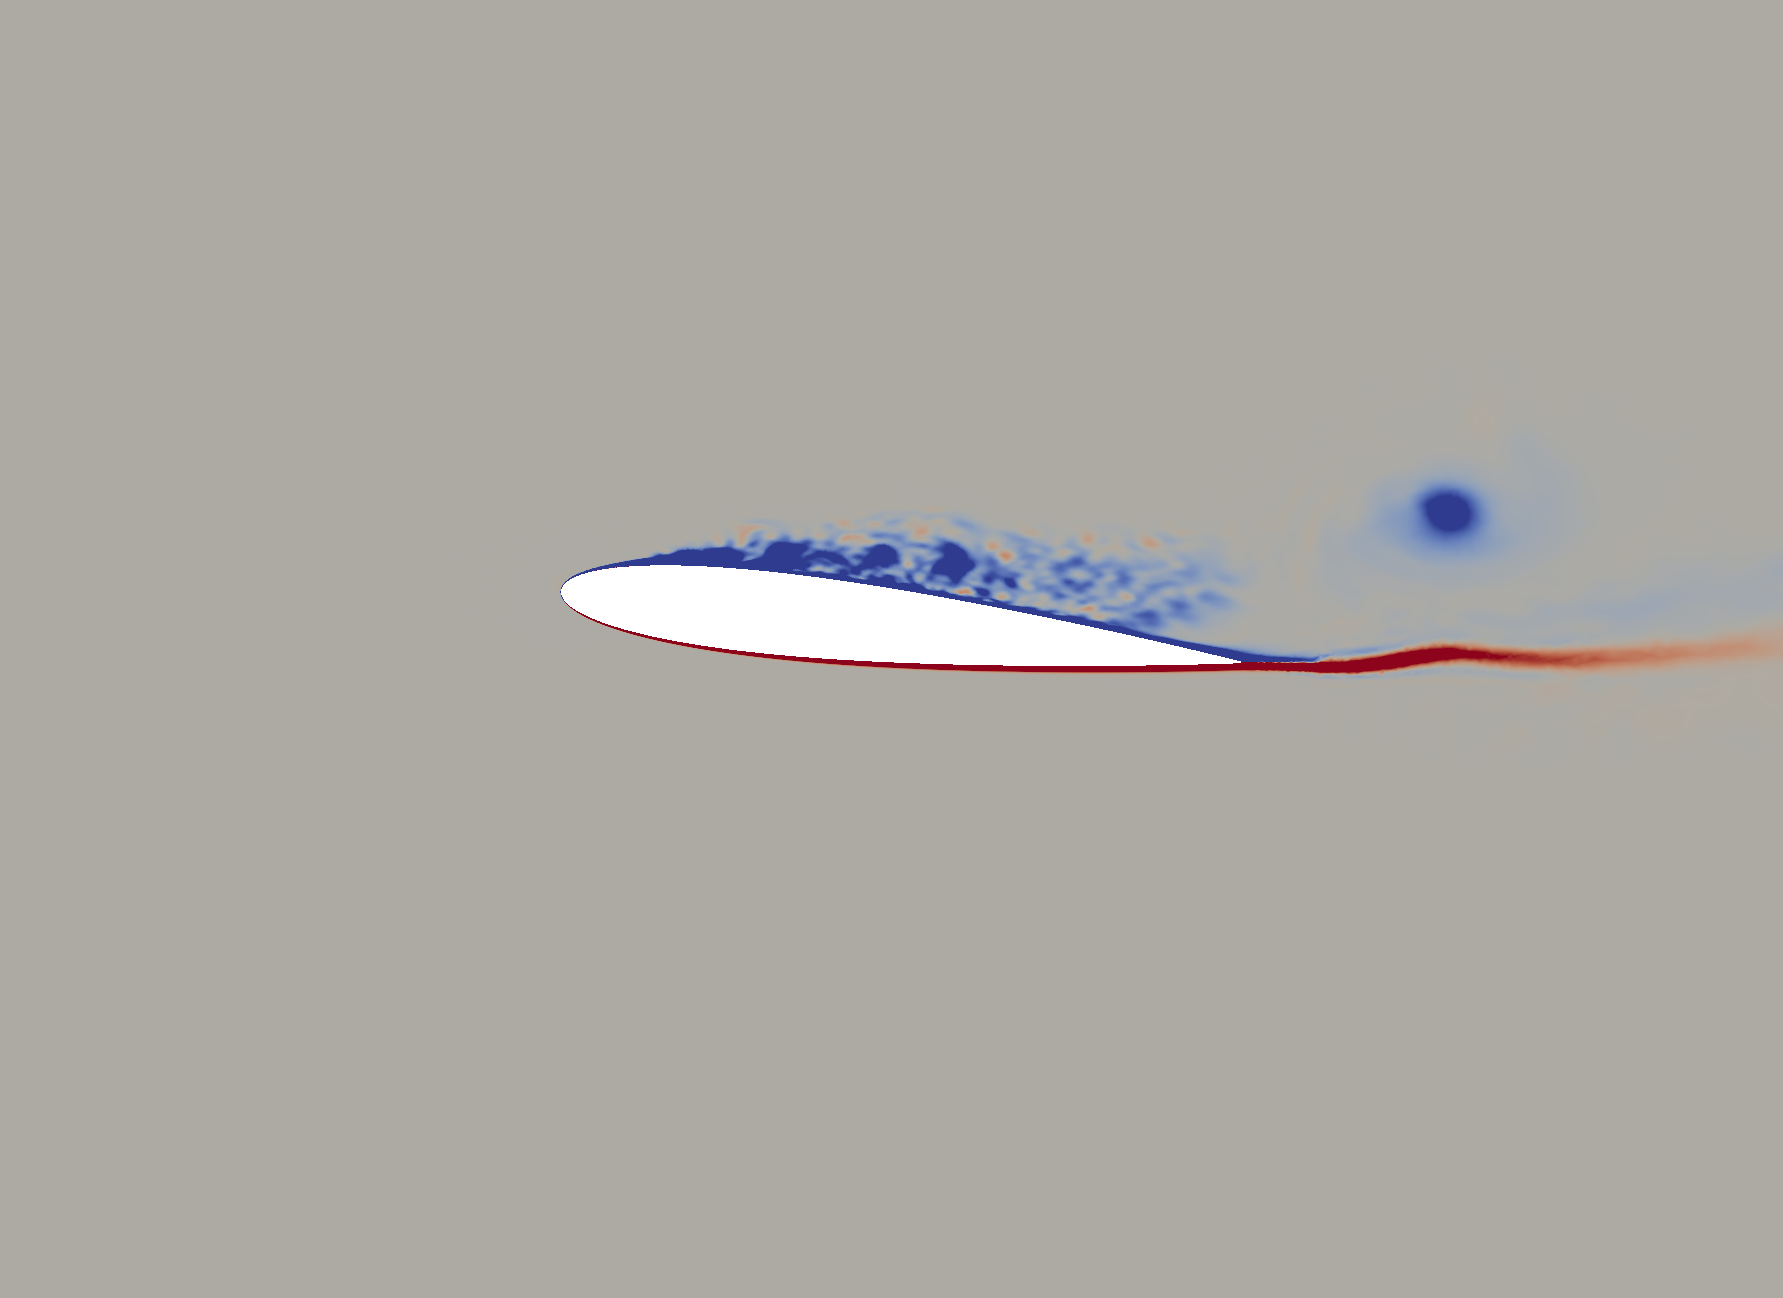
\includegraphics[width=1\textwidth]{figures/Vorticity_plots/Re_200k_1pt0/phase_345.png}
		\caption{$Re=2e5$, $\psi$ = $345^\circ$, $\tilde{t}=0.958$}
		\label{fig:Re_200k_1pt0_phi345}
	\end{subfigure}
	\begin{subfigure}[b]{0.32\textwidth}
		\centering
		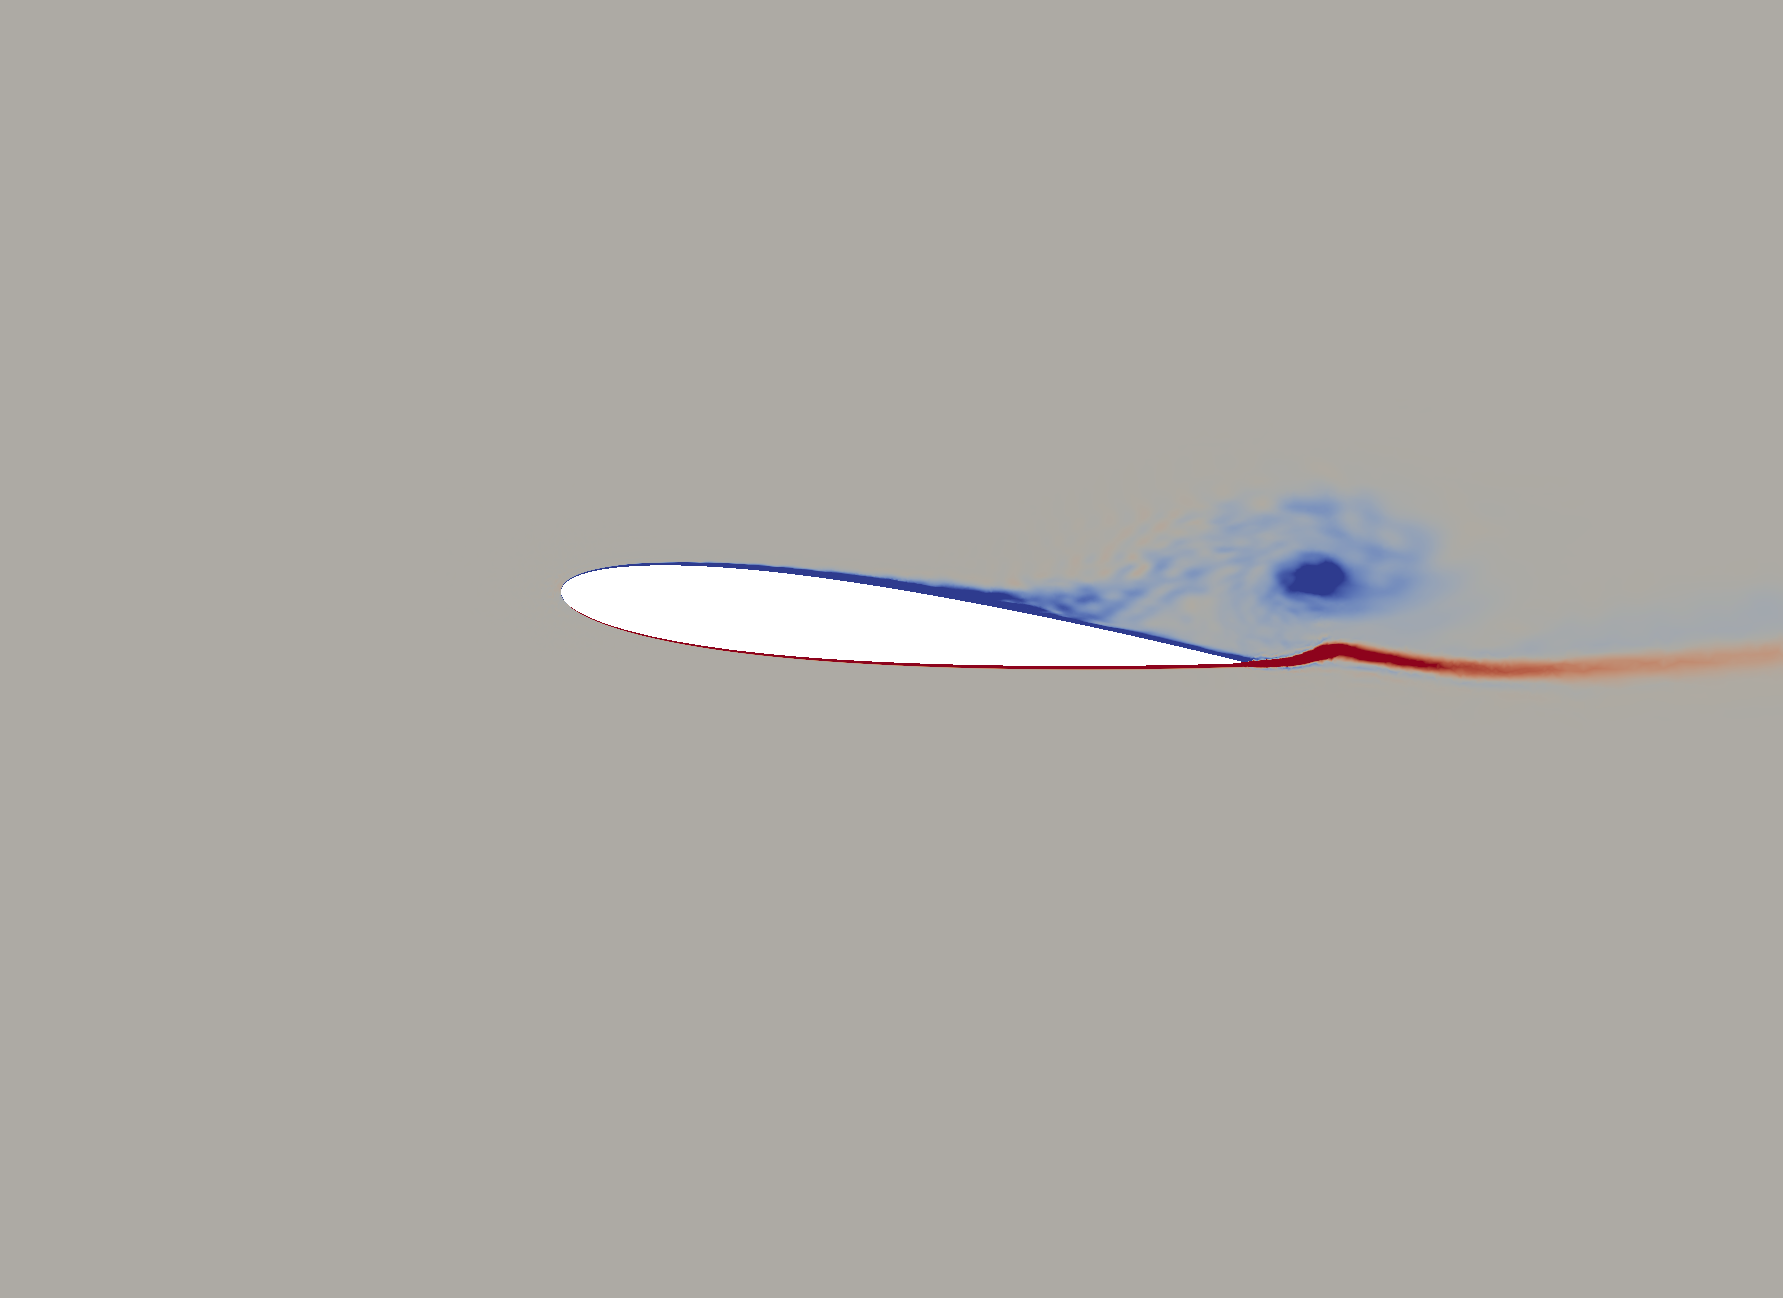
\includegraphics[width=1\textwidth]{figures/Vorticity_plots/Re_1m_1pt0/phase_345.png}
		\caption{$Re=1e6$, $\psi$ = $345^\circ$, $\tilde{t}=0.958$}
		\label{fig:Re_1m_1pt0_phi345}
	\end{subfigure}	
\caption{Spanwise vorticity at 8 different phases for $Re$=40,000 (left column), 200,000 (middle column) and 1,000,000 (right column) at $\mu_{sect}$ = 1.0}
\label{fig:vortScreen_1pt0}
\end{figure}


At $\psi$=$225^\circ$, the flow is separated near the leading edge for the lowest Reynolds number of $Re$=40,000 and the separated shear layer rolls up into an LEV, see Figure~\ref{fig:Re_200k_1pt0_phi225}.
For the other two higher Reynolds numbers, the flow remains attached.
Similarly, at $Re$=200,000 the separated shear layer rolls up into a smaller LEV at $\psi$=$240^\circ$, while for $Re$=1,000,000 this occurs at $\psi$=$270^\circ$ (see Figure \ref{fig:Re_1m_1pt0_phi270}).
As the Reynolds number increases the LEV is formed later in the cycle.
In summary, as the airfoil retreats vorticity accumulates around the airfoil and separated shear layer rolls up into a distinct vortex near the leading edge (i.e., an LEV) over the suction or upper side of the airfoil.

In subsequent phases, LEV is ejected into the outer flow and advects.
The flow on the suction or upper side reattaches as the leading edge vortex passes over the airfoil.
Flow also separates and reattaches on the pressure or lower side, e.g., see marginal flow separation at the trailing edge on the lower side in Fig \ref{fig:Re_40k_1pt0_phi225}.

It is important to note the differences in LEV evolution with different Reynolds number even though the overall trend of the LEV evolution is similar between different Reynolds number.
As already noted, the phase at which the LEV is formed changes with Reynolds number.
Further, the size and vertical position of the LEV also changes significantly with Reynolds number.
This aspect is discussed in Section \ref{sec:LEV}.

Figure \ref{fig:vortScreen_1pt2} shows the spanwise vorticity for the higher advance ratio of $\mu_{sect}$=1.2.
Again, 8 different phases over the retreating phase of the cycle are shown and the range is selected to be [-10,10]$\times U_\infty /C$.
As in the $\mu_{sect}=1.0$ case, at $\psi$=$195^\circ$ the flow over the airfoil is mostly attached in the $\mu_{sect}=1.2$ case.
As before, the boundary layer is much thicker for the lowest Reynolds number of $Re$=40,000 as compared to the other two higher Reynolds numbers.

At $\psi$=$225^\circ$, the flow is fully separated for the lowest Reynolds number of $Re$=40,000 and the separated shear layer is rolled up into an LEV, see Figure~\ref{fig:Re_40k_1pt2_phi225}.
Similarly, at $Re$=200,000 a smaller LEV is seen at $\psi$=$225^\circ$ (see Figure \ref{fig:Re_200k_1pt2_phi225}), while for $Re$=1,000,000, LEV is observed at $\psi$=$240^\circ$.
As before, as the Reynolds number increases the LEV is formed later in the cycle.
On the other hand, as the advance ratio increases it is formed earlier in the cycle (for a given Reynolds number).
For example, for $Re$=1,000,000, the LEV is formed at an earlier phase for $\mu_{sect}=1.2$ as compared to $\mu_{sect}=1.0$.
Again, as the airfoil retreats vorticity accumulates and shear layer rolls up into a distinct LEV over the suction or upper side of the airfoil.

In subsequent phases, LEV is ejected into the outer flow and advects while the flow reattaches.
However, at the higher advance ratio of $\mu_{sect}$=1.2 the LEV initially moves to the left past the (geometric) leading edge of the airfoil.
This is because at $\mu_{sect}$=1.2, the relative flow velocity becomes negative and a reversed flow condition is reached.
Again, it is important to note the differences in LEV evolution with different Reynolds number for the advance ratio of $\mu_{sect}=1.2$.
As already noted, the size, position and phase of formation of LEV changes significantly with Reynolds number.
This aspect is discussed further in Section \ref{sec:LEV}.

\begin{figure}[H]
	\centering
	
	\begin{subfigure}[b]{0.32\textwidth}
		\centering
		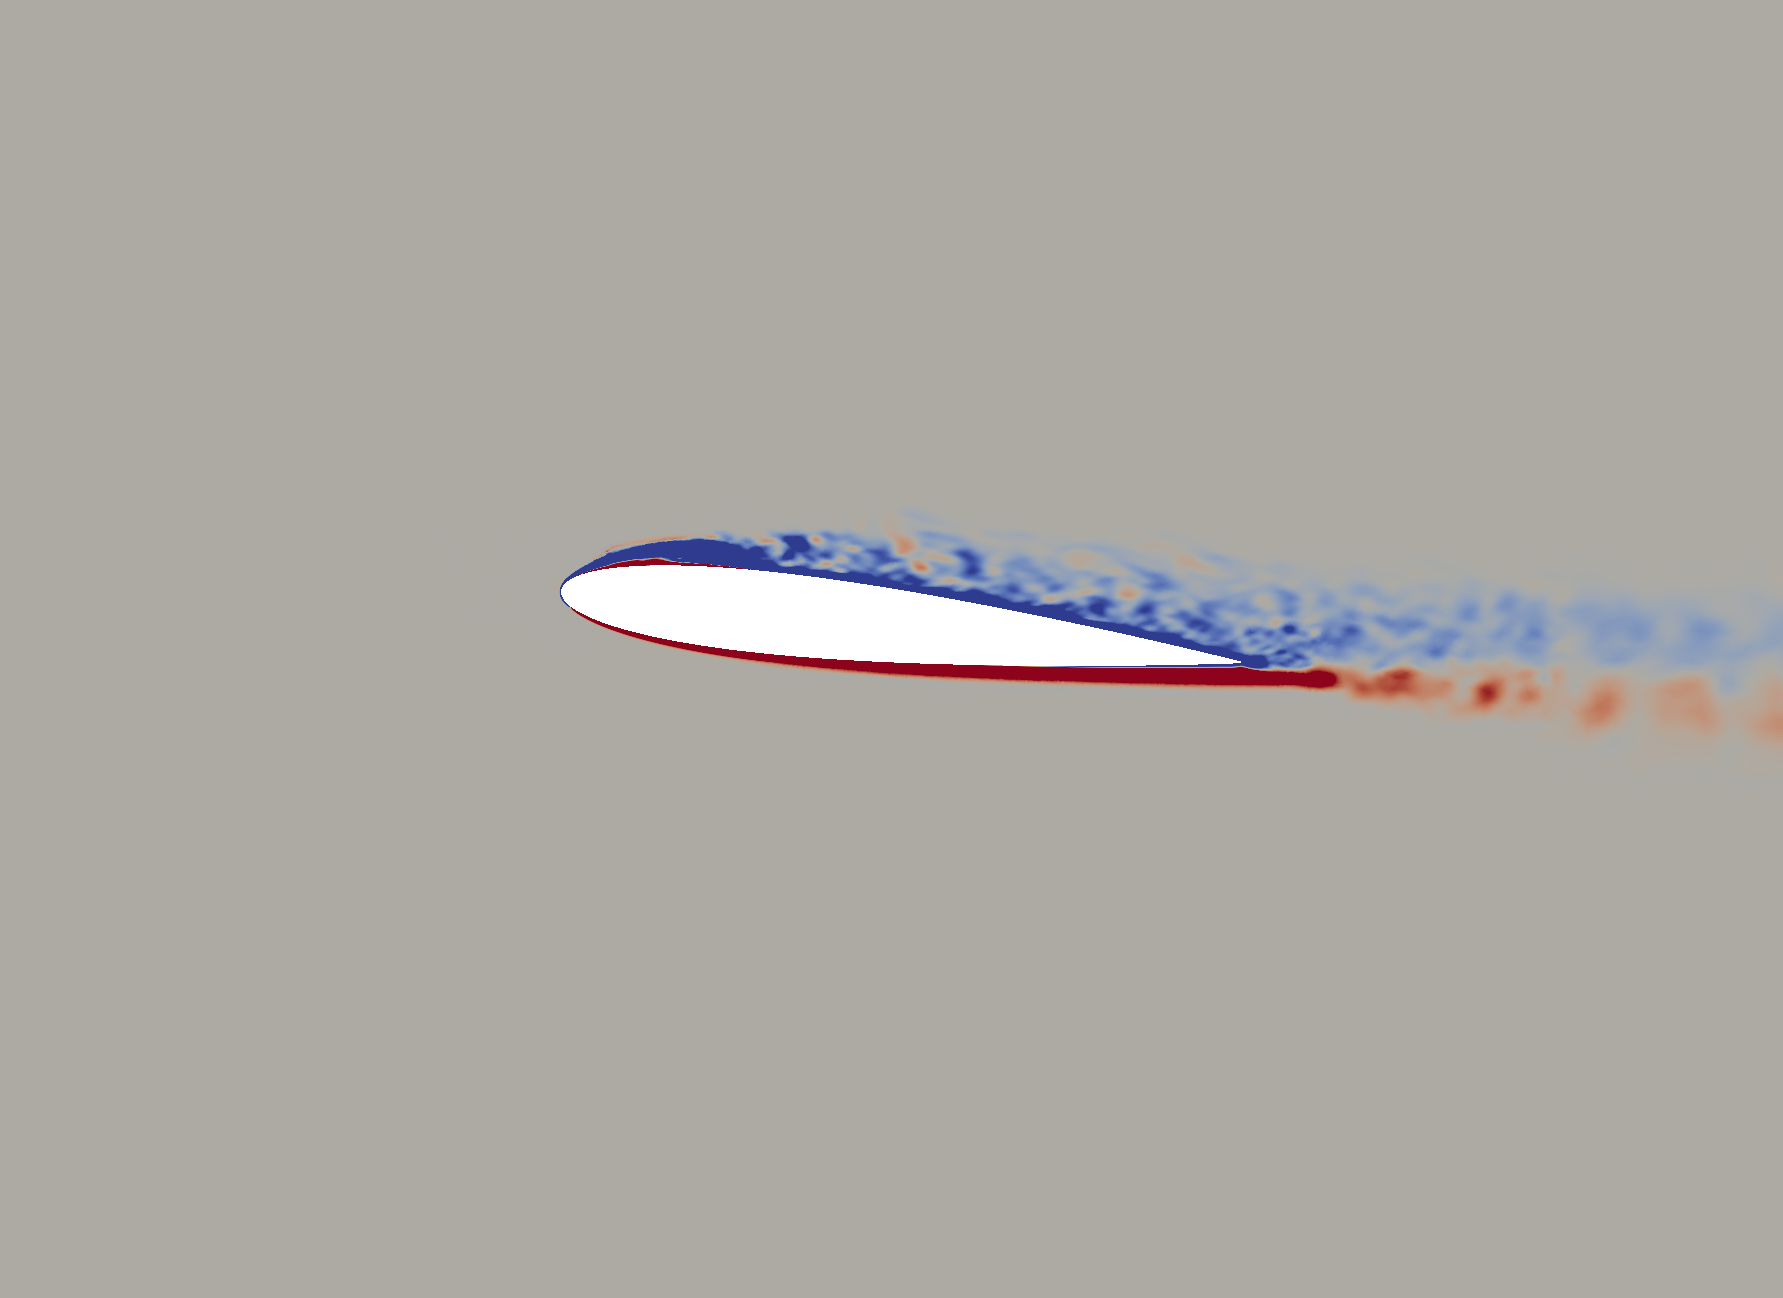
\includegraphics[width=1\textwidth]{figures/Vorticity_plots/Re_40k_1pt2/phase_195.png}
		\caption{$Re= 4e4$, $\psi$ = $195^\circ$, $\tilde{t}=0.542$}
		\label{fig:Re_40k_1pt2_phi195}
	\end{subfigure}
	\begin{subfigure}[b]{0.32\textwidth}
		\centering
		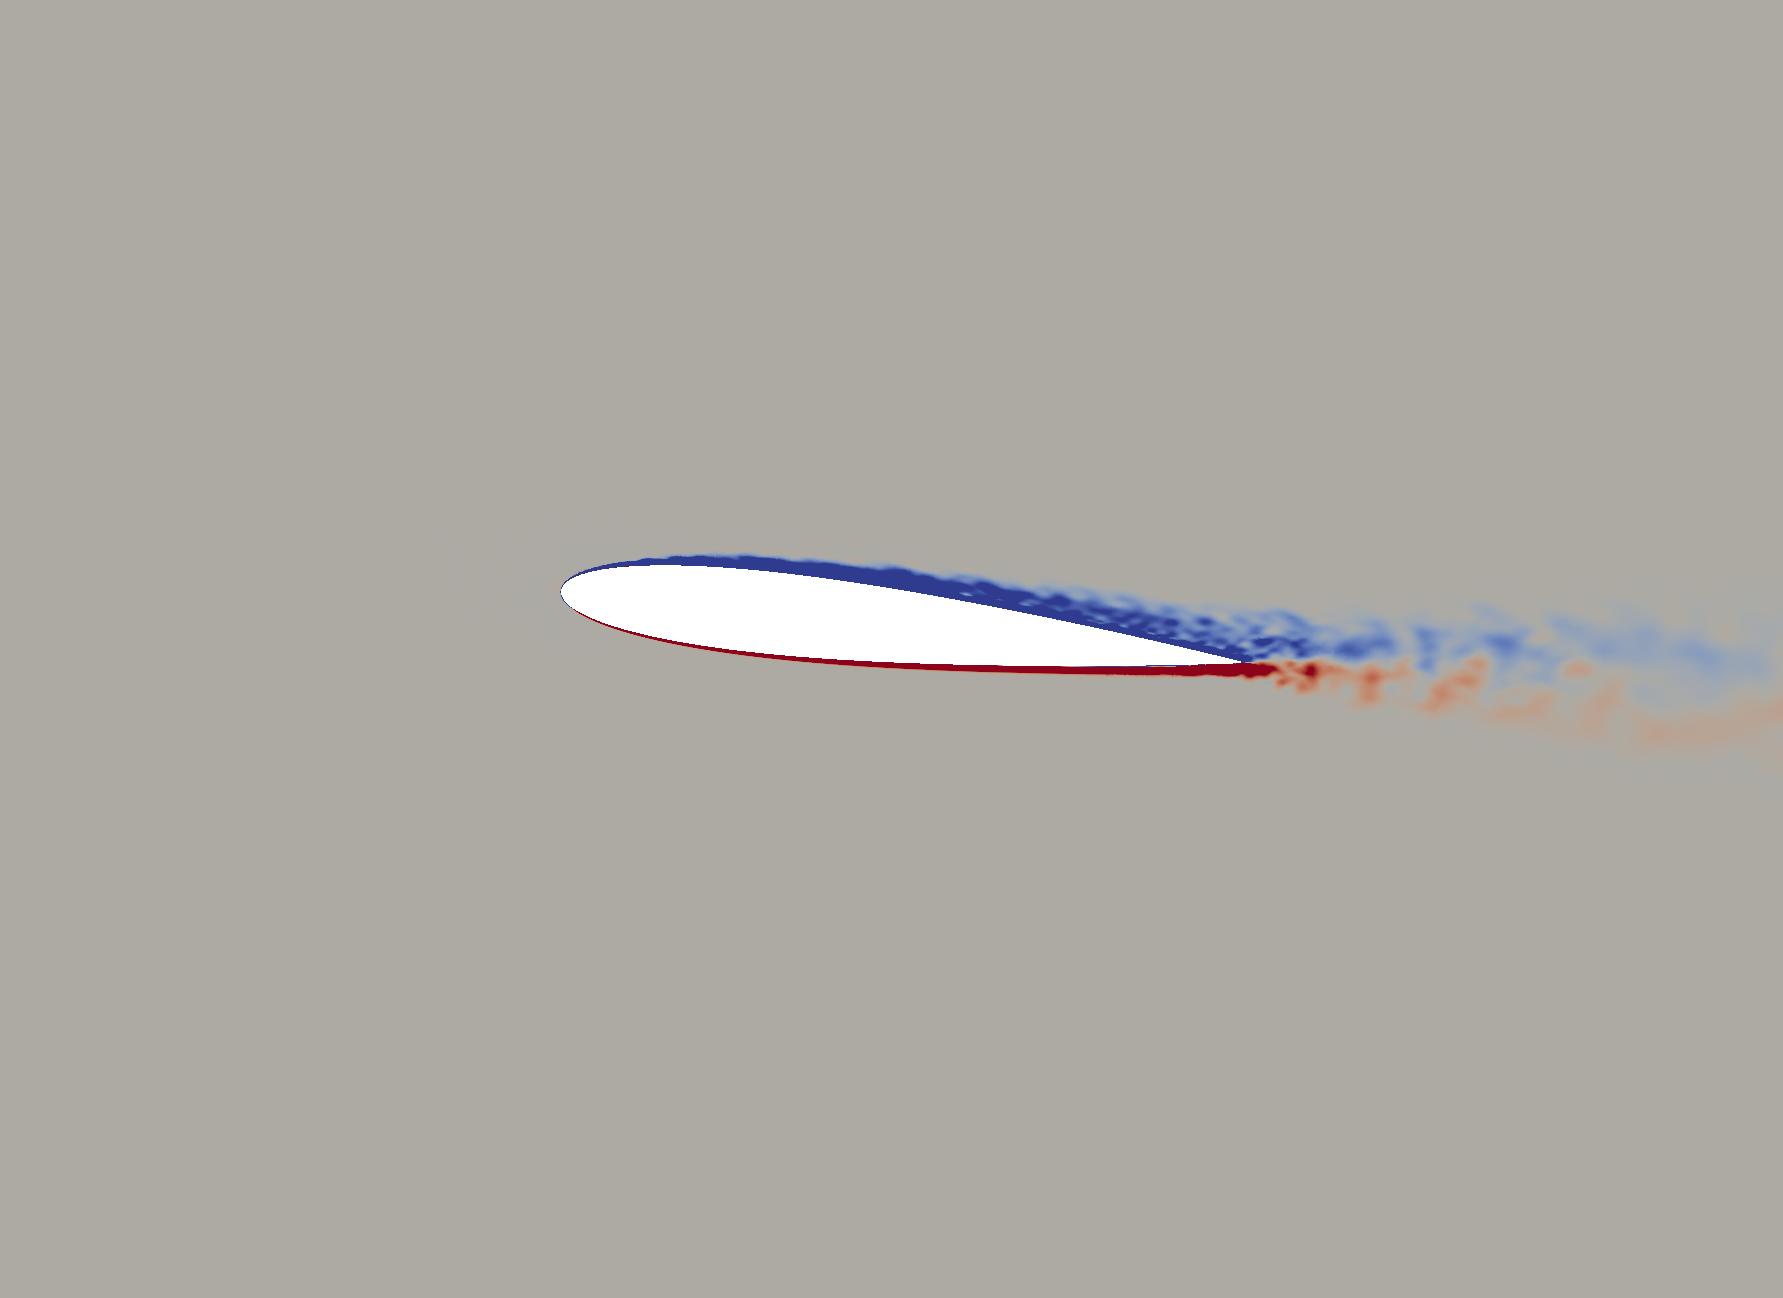
\includegraphics[width=1\textwidth]{figures/Vorticity_plots/Re_200k_1pt2/phase_195.png}
		\caption{$Re=2e5$, $\psi$ = $195^\circ$, $\tilde{t}=0.542$}
		\label{fig:Re_200k_1pt2_phi195}
	\end{subfigure}
	\begin{subfigure}[b]{0.32\textwidth}
		\centering
		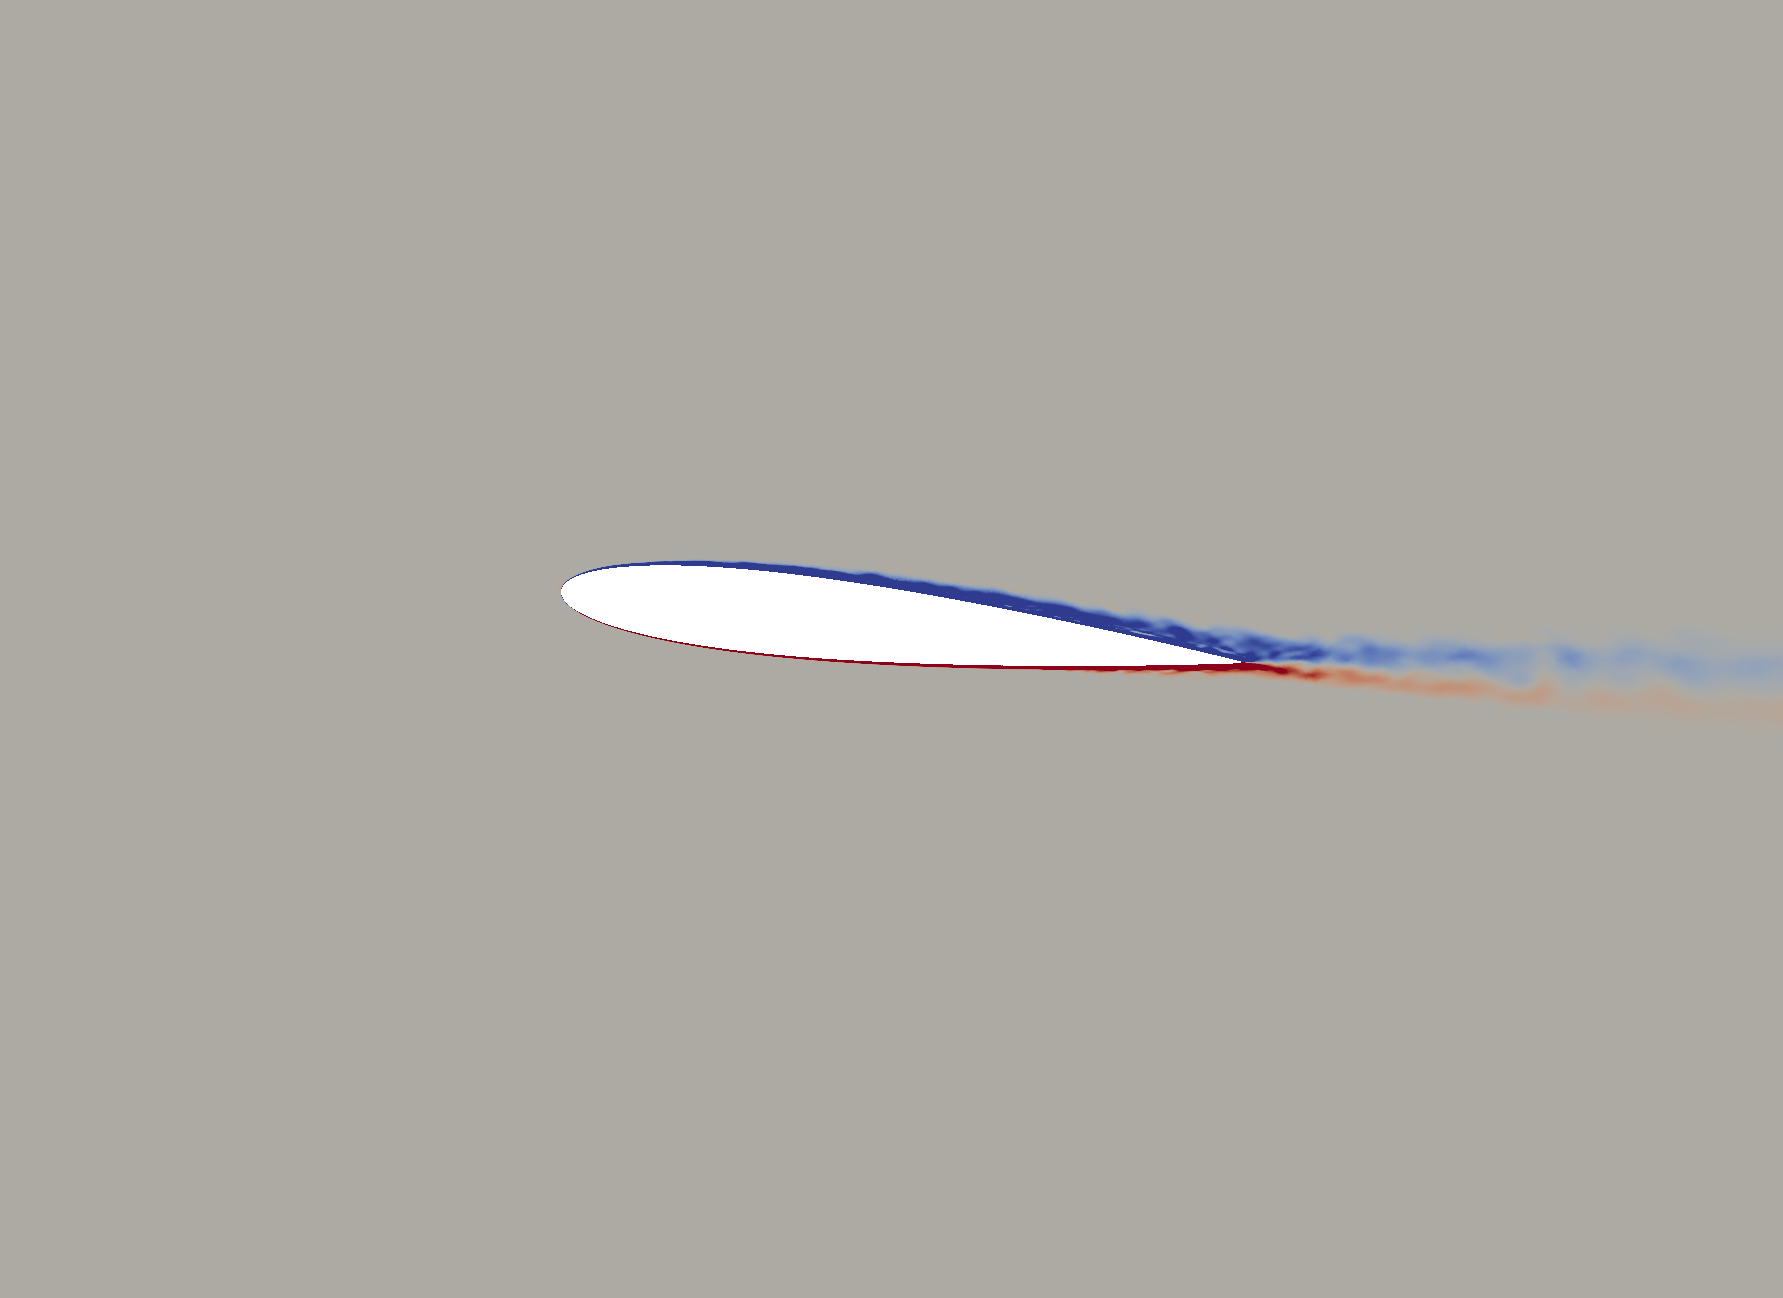
\includegraphics[width=1\textwidth]{figures/Vorticity_plots/Re_1m_1pt2/phase_195.png}
		\caption{$Re= 1e6$, $\psi$ = $195^\circ$, $\tilde{t}=0.542$}
		\label{fig:Re_1m_1pt2_phi195}
	\end{subfigure}
	
	\begin{subfigure}[b]{0.32\textwidth}
		\centering
		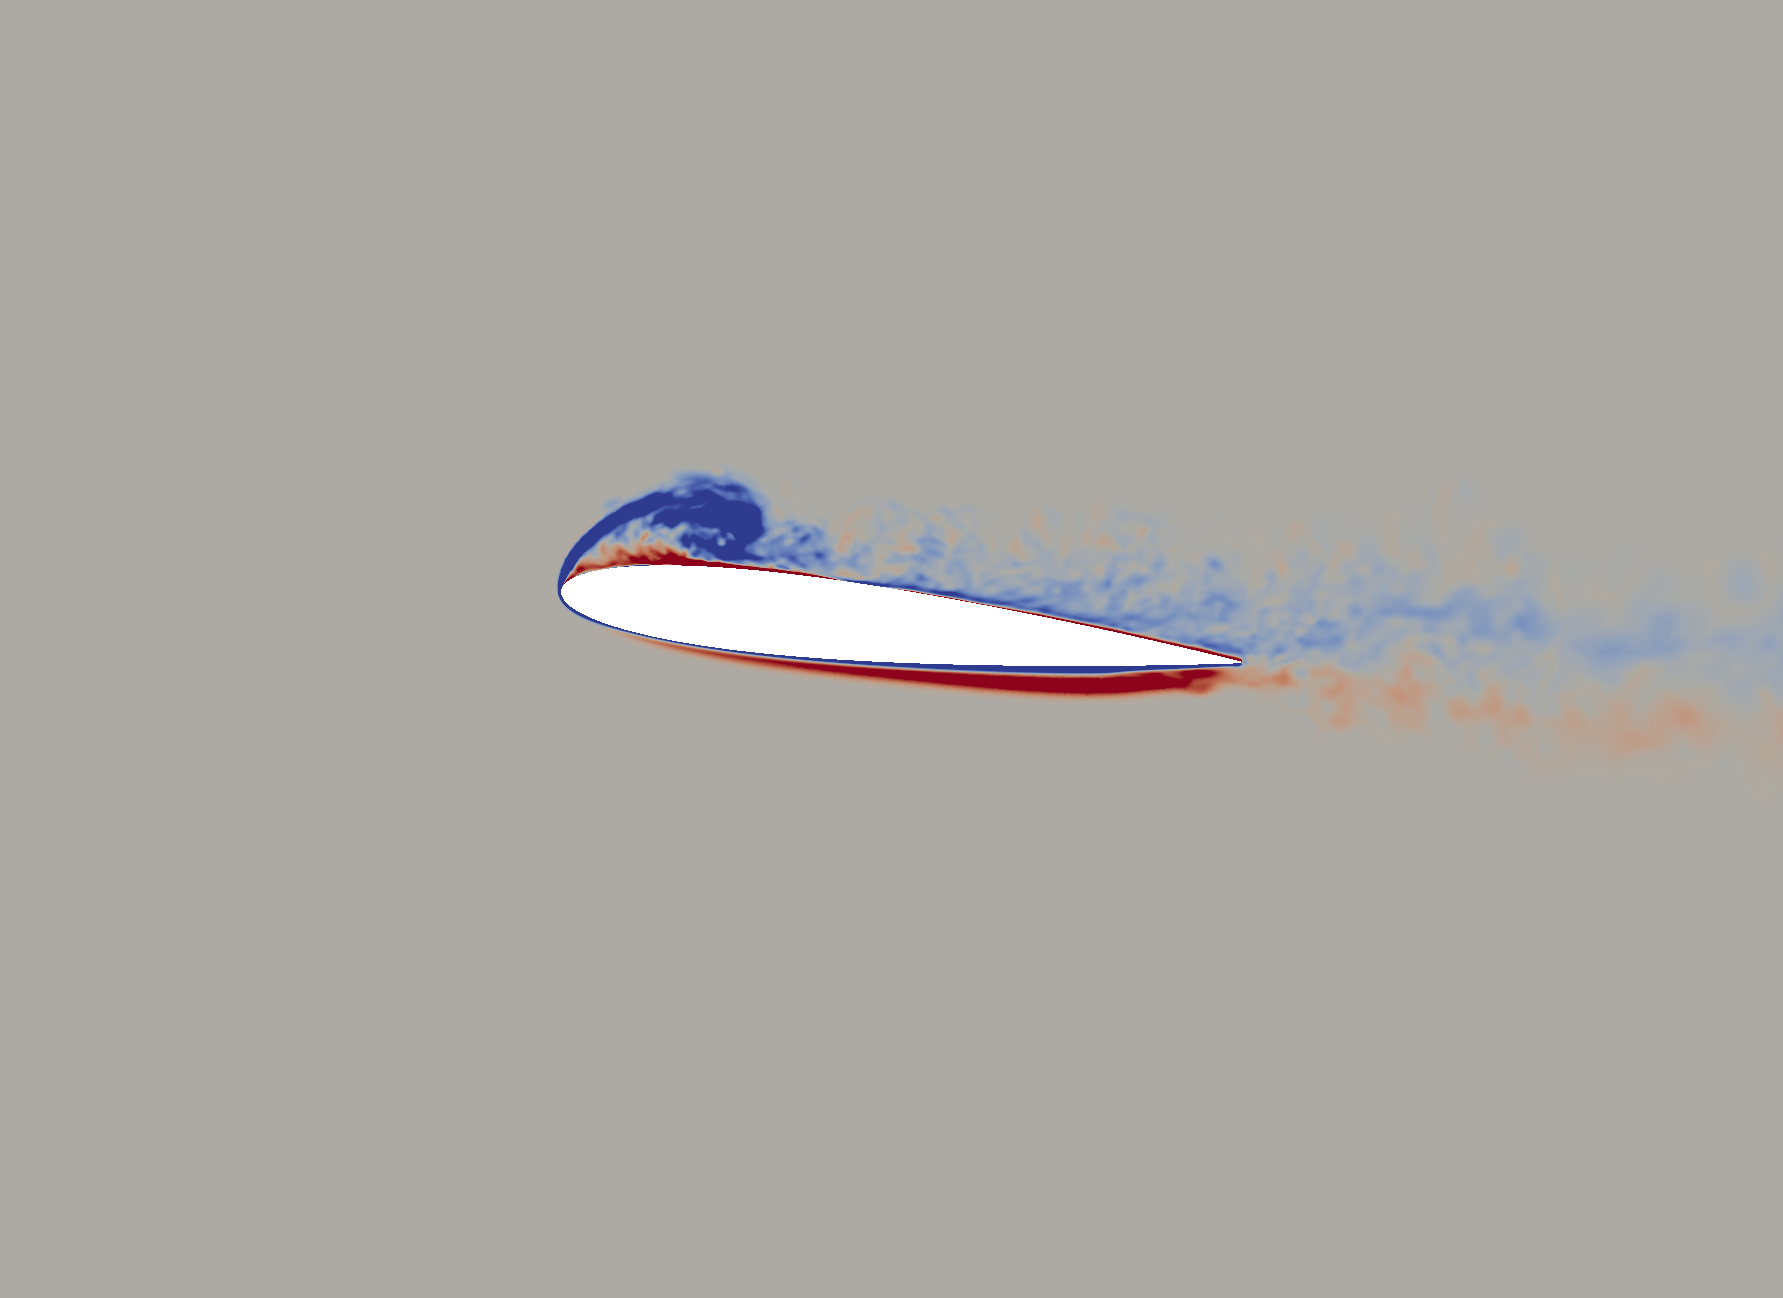
\includegraphics[width=1\textwidth]{figures/Vorticity_plots/Re_40k_1pt2/phase_225.png}
		\caption{$Re=4e4$, $\psi$ = $225^\circ$, $\tilde{t}=0.625$}
		\label{fig:Re_40k_1pt2_phi225}
	\end{subfigure}
	\begin{subfigure}[b]{0.32\textwidth}
		\centering
		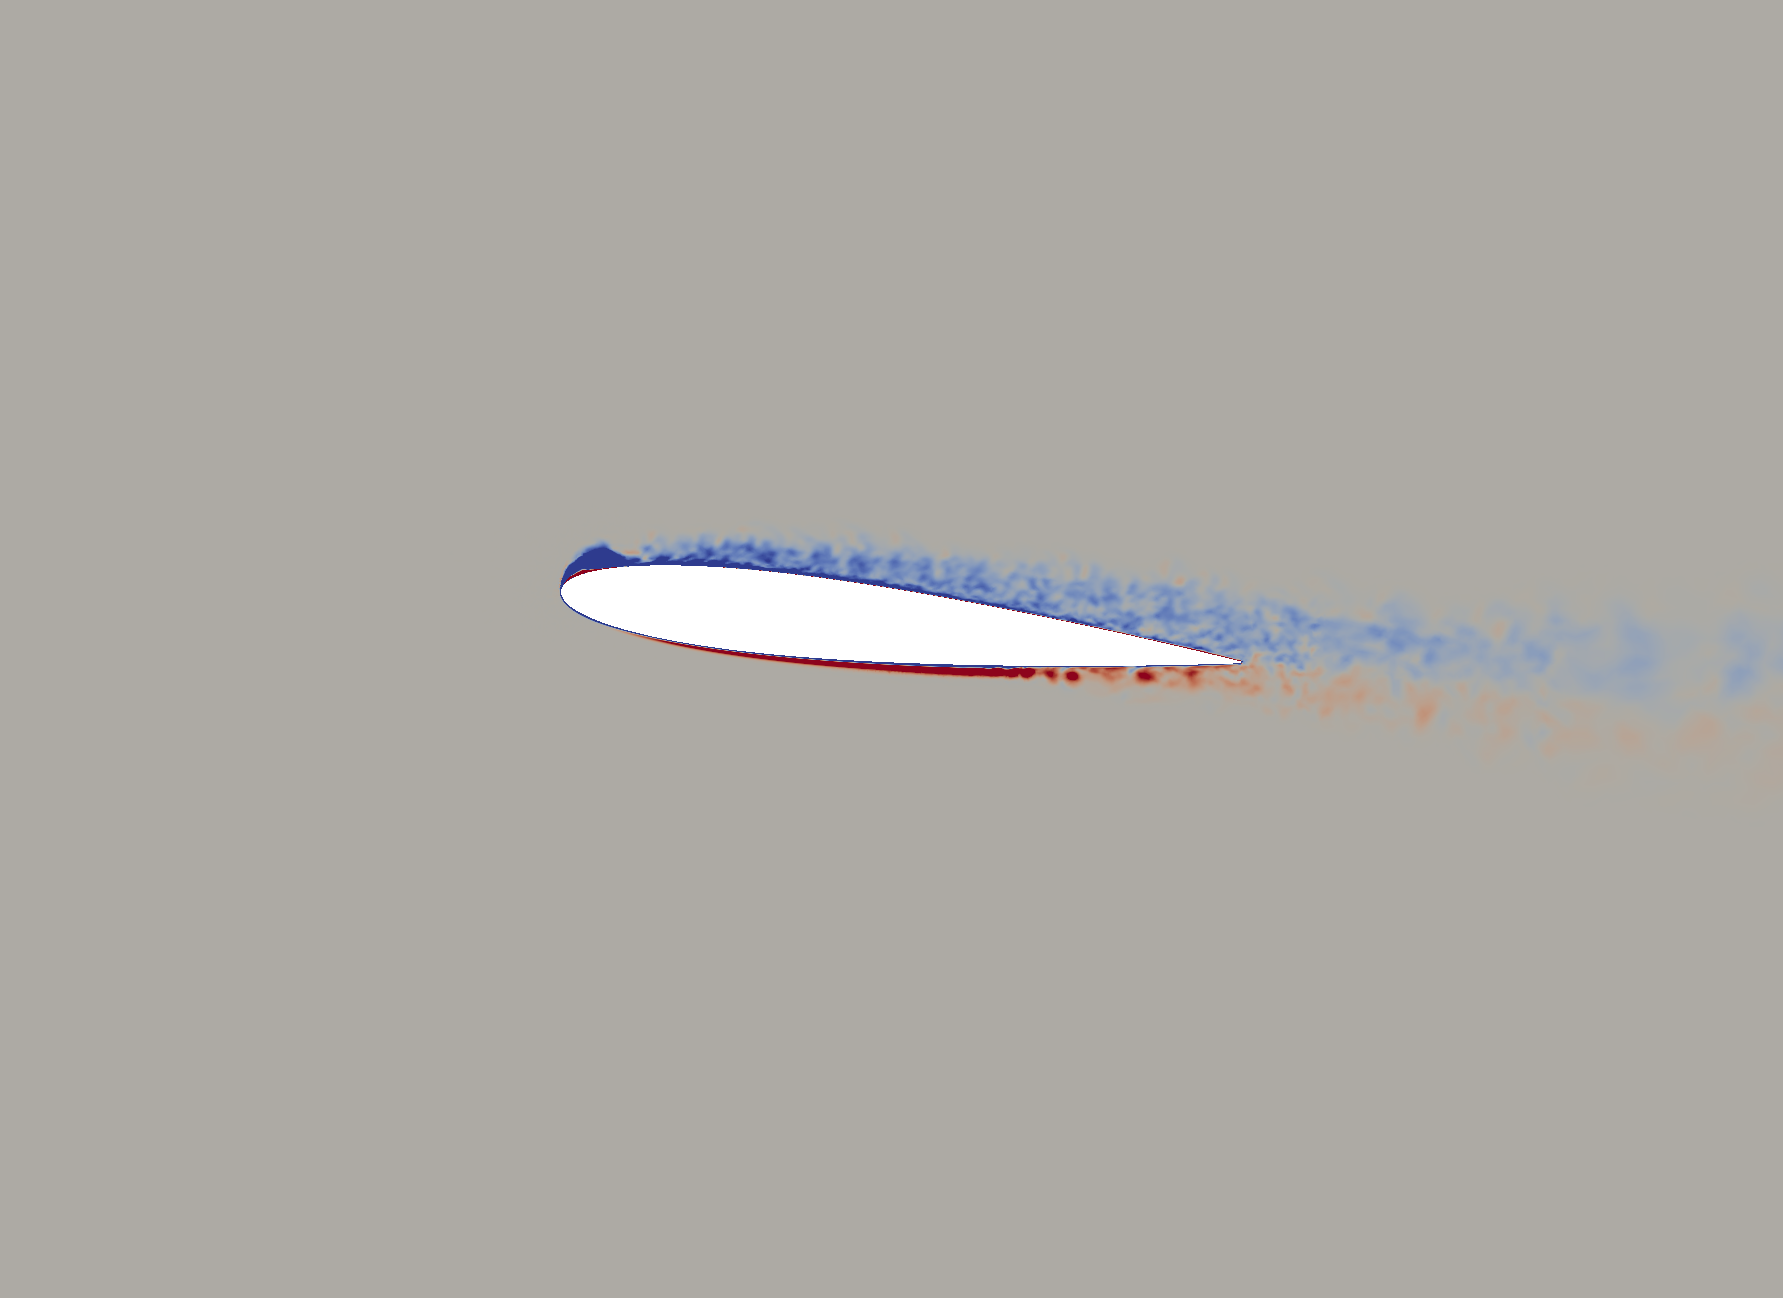
\includegraphics[width=1\textwidth]{figures/Vorticity_plots/Re_200k_1pt2/phase_225.png}
		\caption{$Re=2e5$, $\psi$ = $225^\circ$, $\tilde{t}=0.625$}
		\label{fig:Re_200k_1pt2_phi225}
	\end{subfigure}
	\begin{subfigure}[b]{0.32\textwidth}
		\centering
		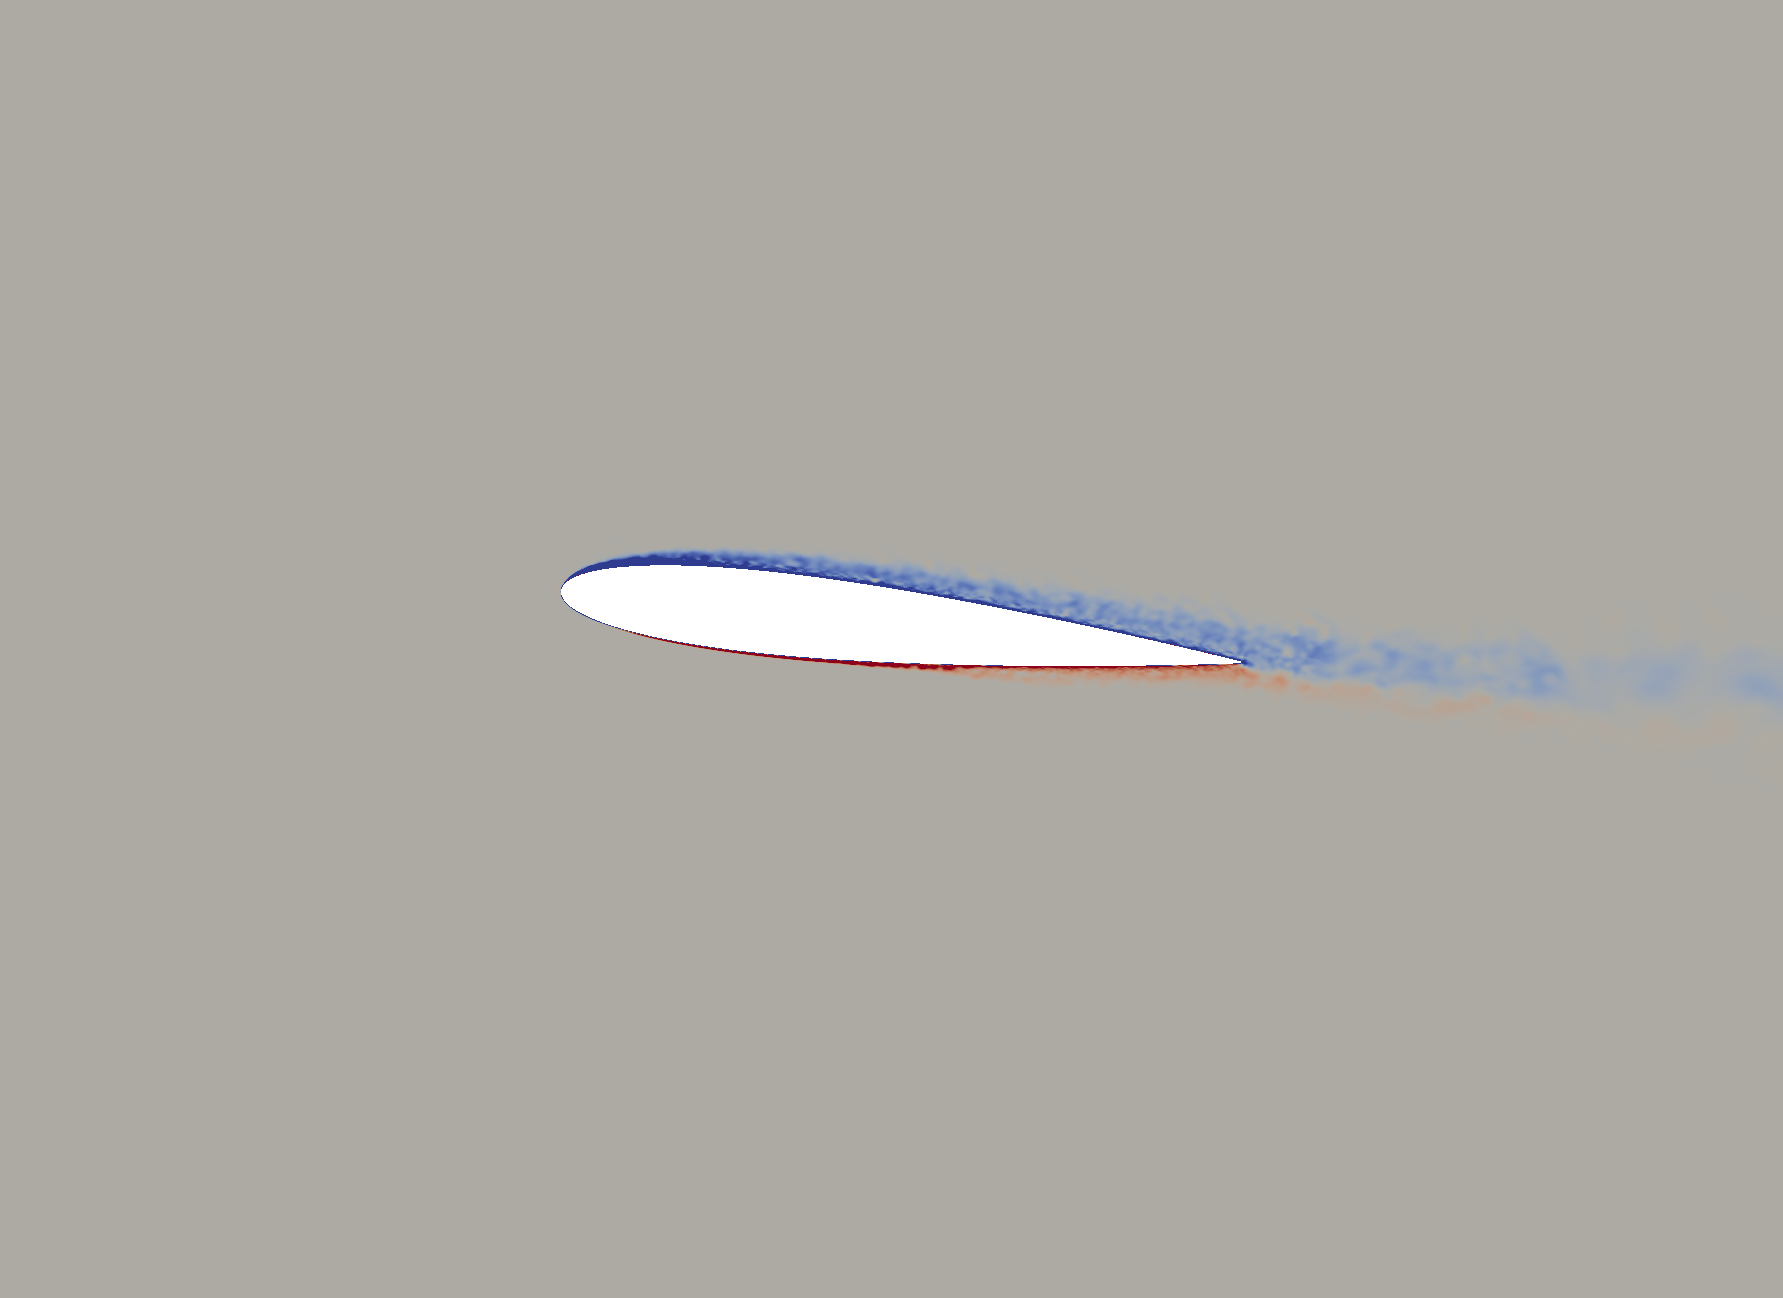
\includegraphics[width=1\textwidth]{figures/Vorticity_plots/Re_1m_1pt2/phase_225.png}
		\caption{$Re=1e6$, $\psi$ = $225^\circ$, $\tilde{t}=0.625$}
		\label{fig:Re_1m_1pt2_phi225}
	\end{subfigure}
	
	\begin{subfigure}[b]{0.32\textwidth}
		\centering
		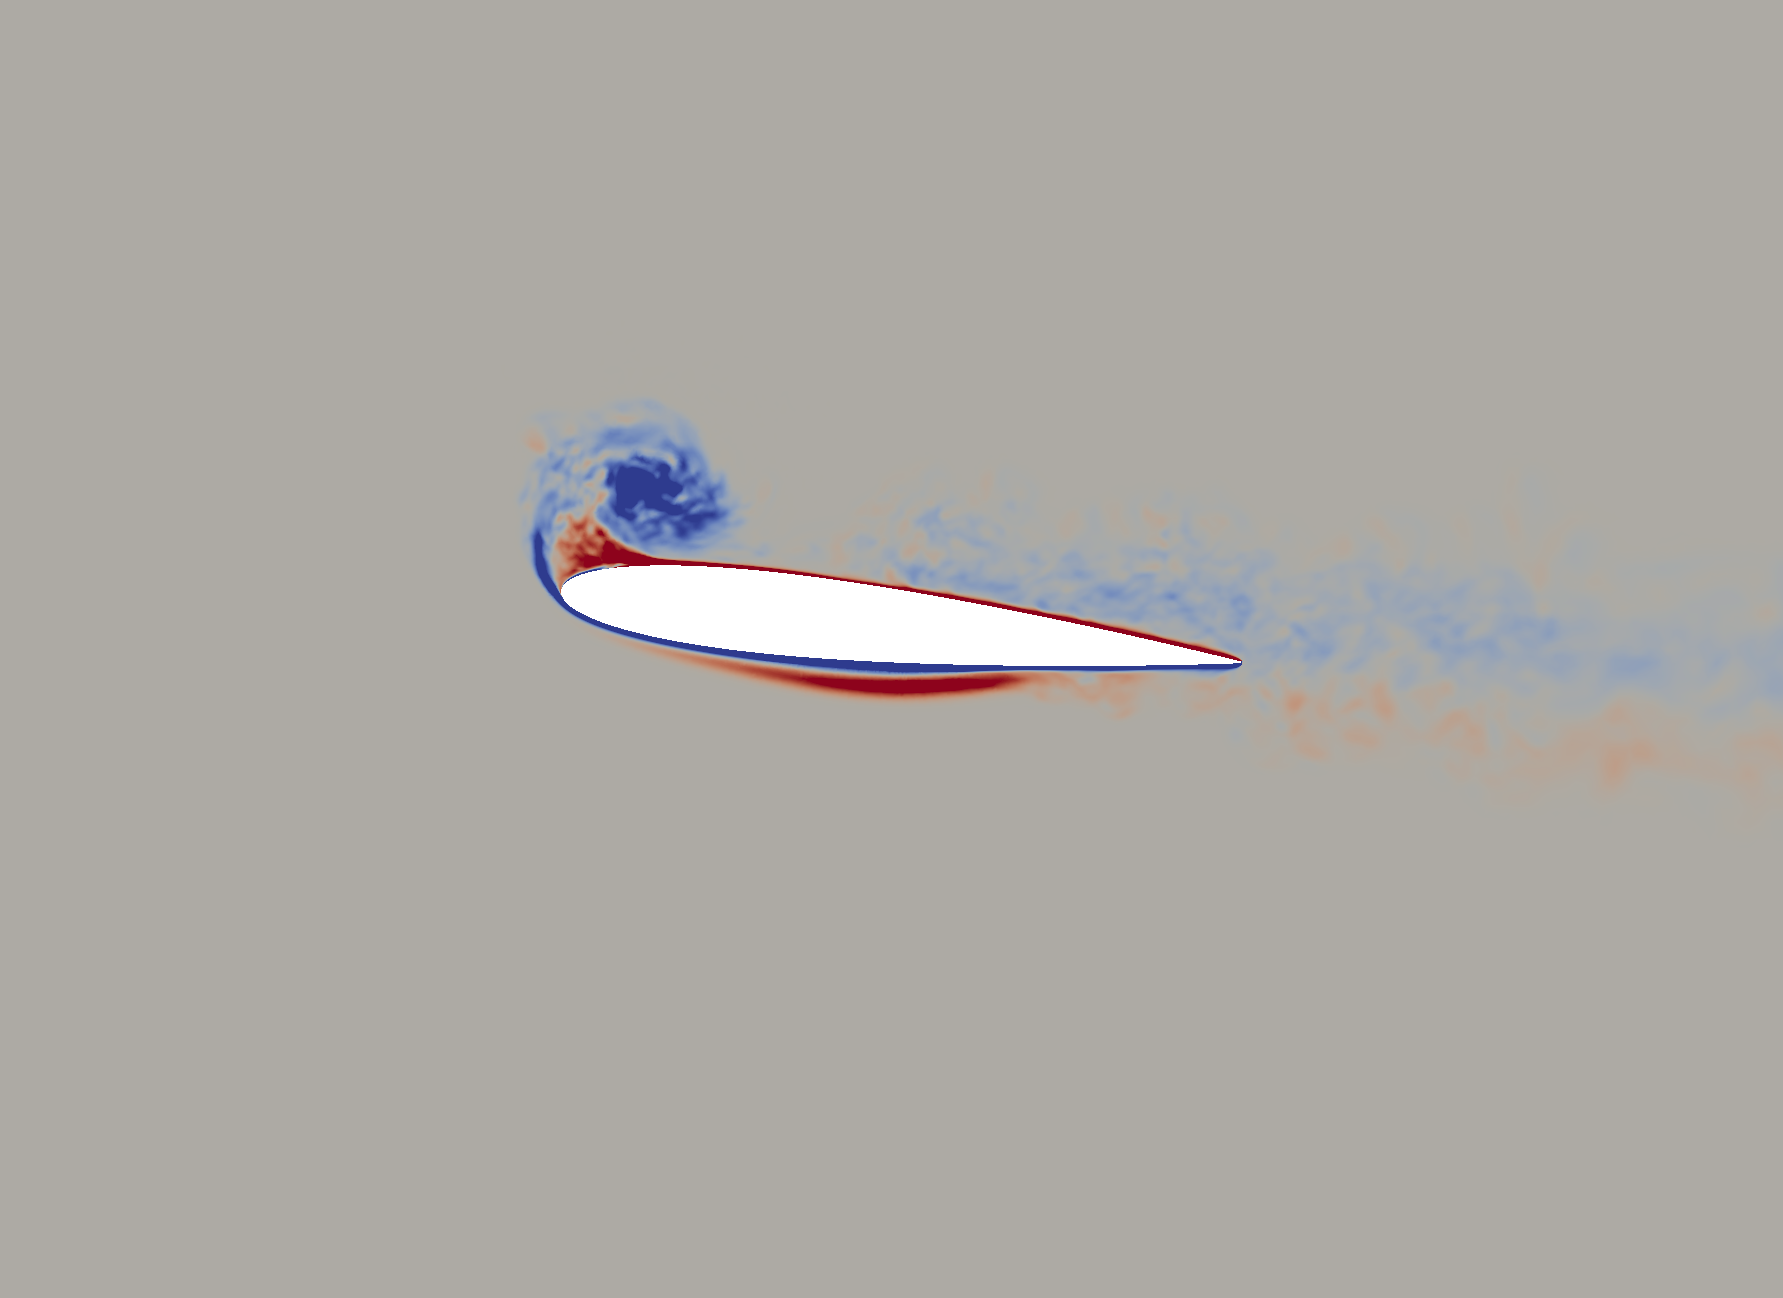
\includegraphics[width=1\textwidth]{figures/Vorticity_plots/Re_40k_1pt2/phase_240.png}
		\caption{$Re=4e4$, $\psi$ = $240^\circ$, $\tilde{t}=0.667$}
		\label{fig:Re_40k_1pt2_phi240}
	\end{subfigure}
	\begin{subfigure}[b]{0.32\textwidth}
		\centering
		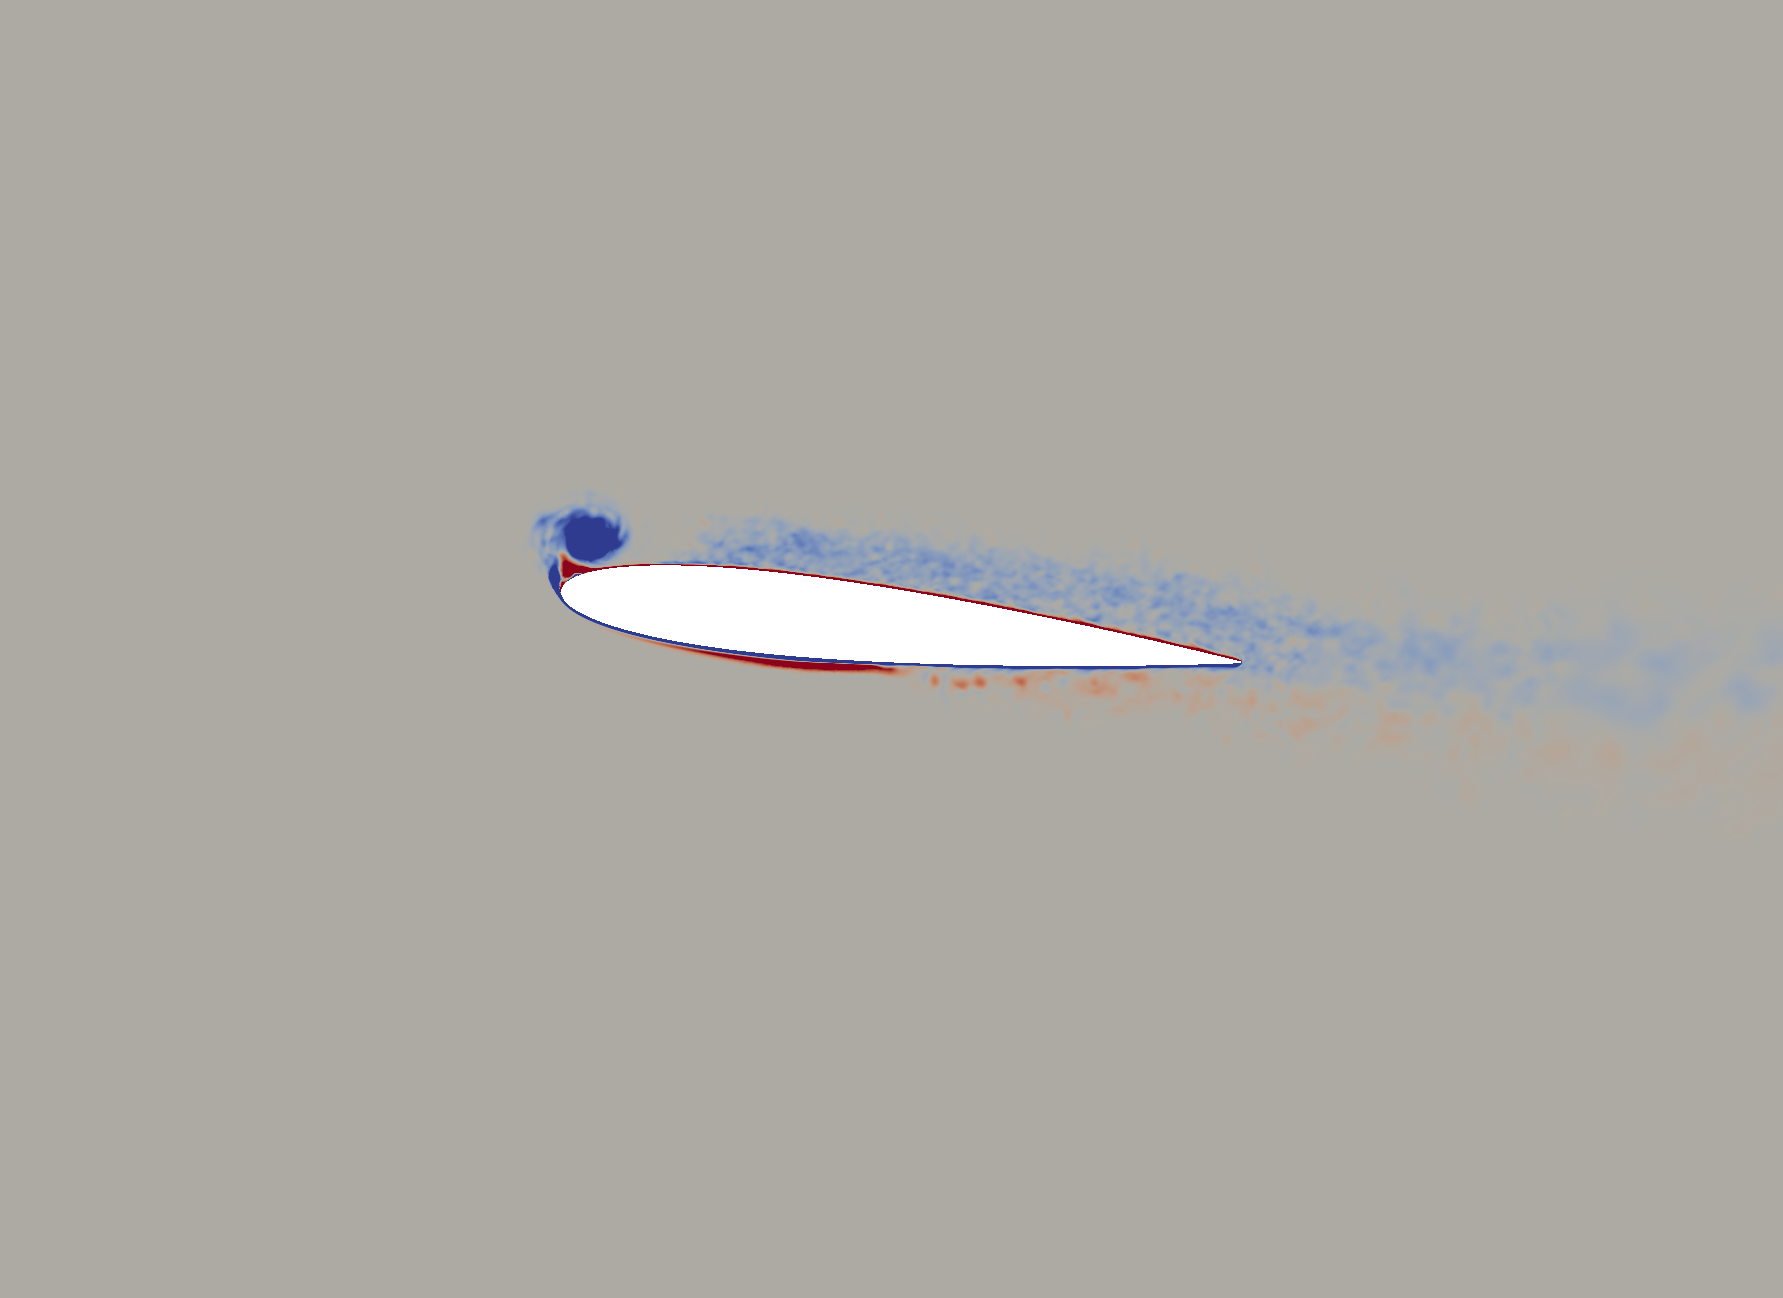
\includegraphics[width=1\textwidth]{figures/Vorticity_plots/Re_200k_1pt2/phase_240.png}
		\caption{$Re=2e5$, $\psi$ = $240^\circ$, $\tilde{t}=0.667$}
		\label{fig:Re_200k_1pt2_phi240}
	\end{subfigure}
	\begin{subfigure}[b]{0.32\textwidth}
		\centering
		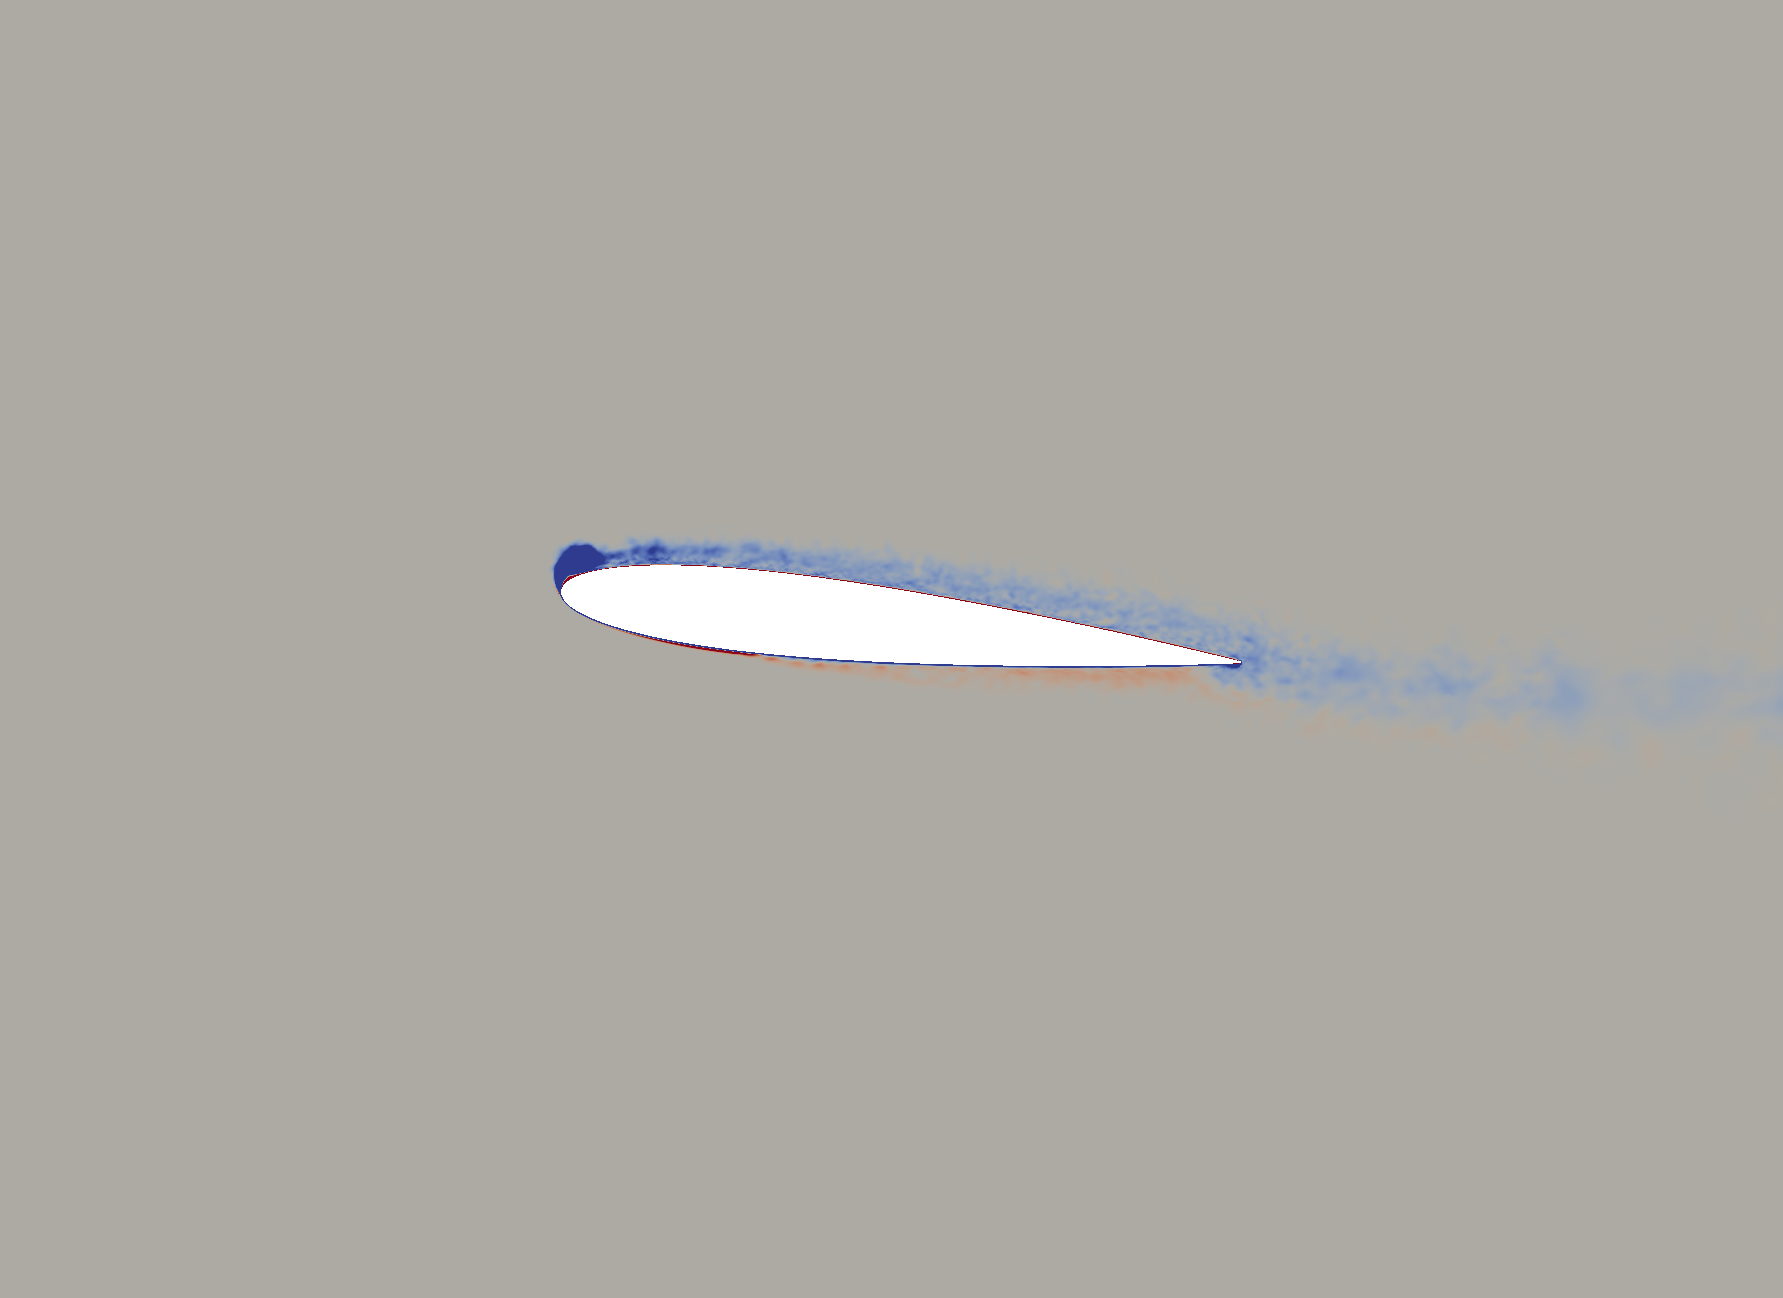
\includegraphics[width=1\textwidth]{figures/Vorticity_plots/Re_1m_1pt2/phase_240.png}
		\caption{$Re=1e6$, $\psi$ = $240^\circ$, $\tilde{t}=0.667$}
		\label{fig:Re_1m_1pt2_phi240}
	\end{subfigure}
	
	\begin{subfigure}[b]{0.32\textwidth}
		\centering
		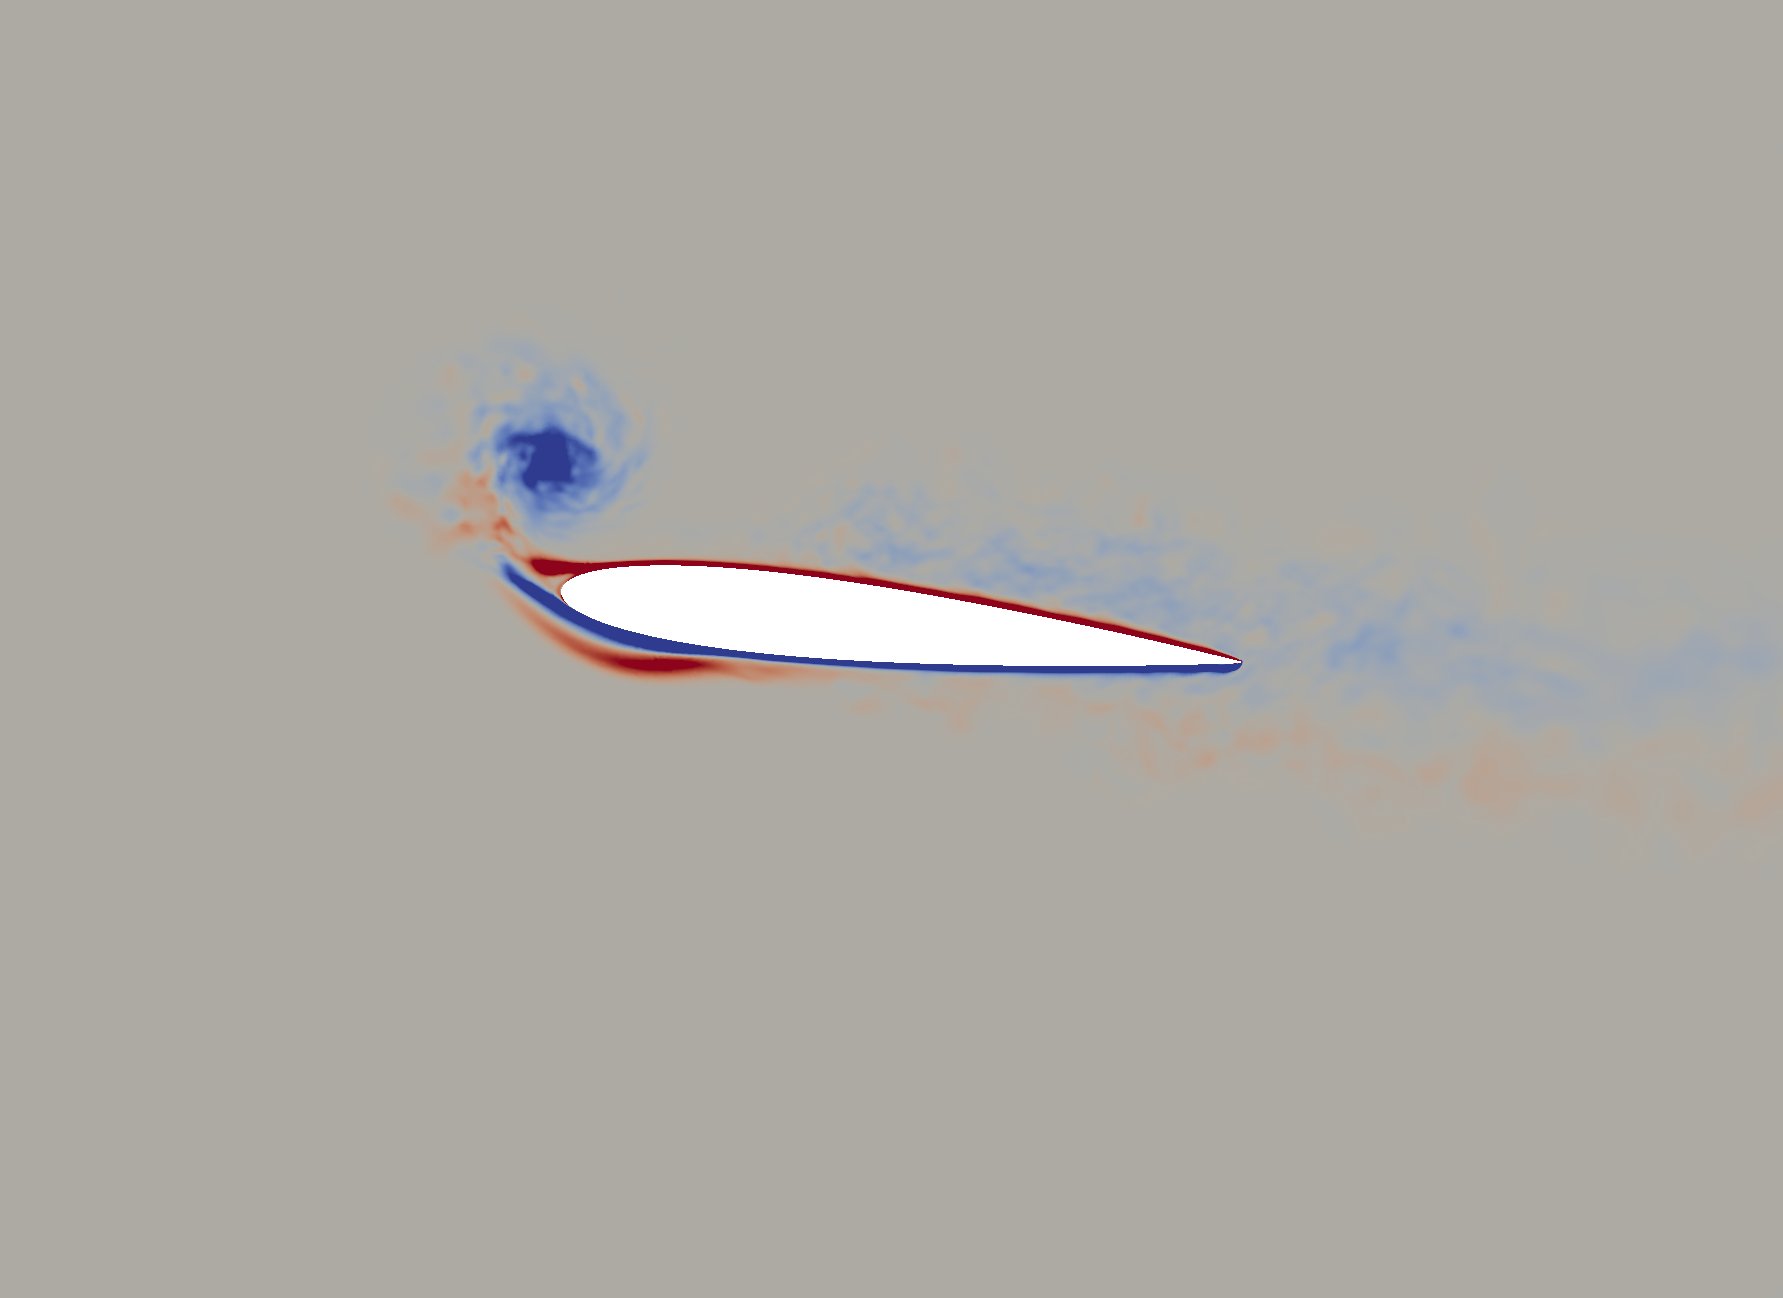
\includegraphics[width=1\textwidth]{figures/Vorticity_plots/Re_40k_1pt2/phase_255.png}
		\caption{$Re=4e4$, $\psi$ = $255^\circ$, $\tilde{t}=0.708$}
		\label{fig:Re_40k_1pt2_phi255}
	\end{subfigure}
	\begin{subfigure}[b]{0.32\textwidth}
		\centering
		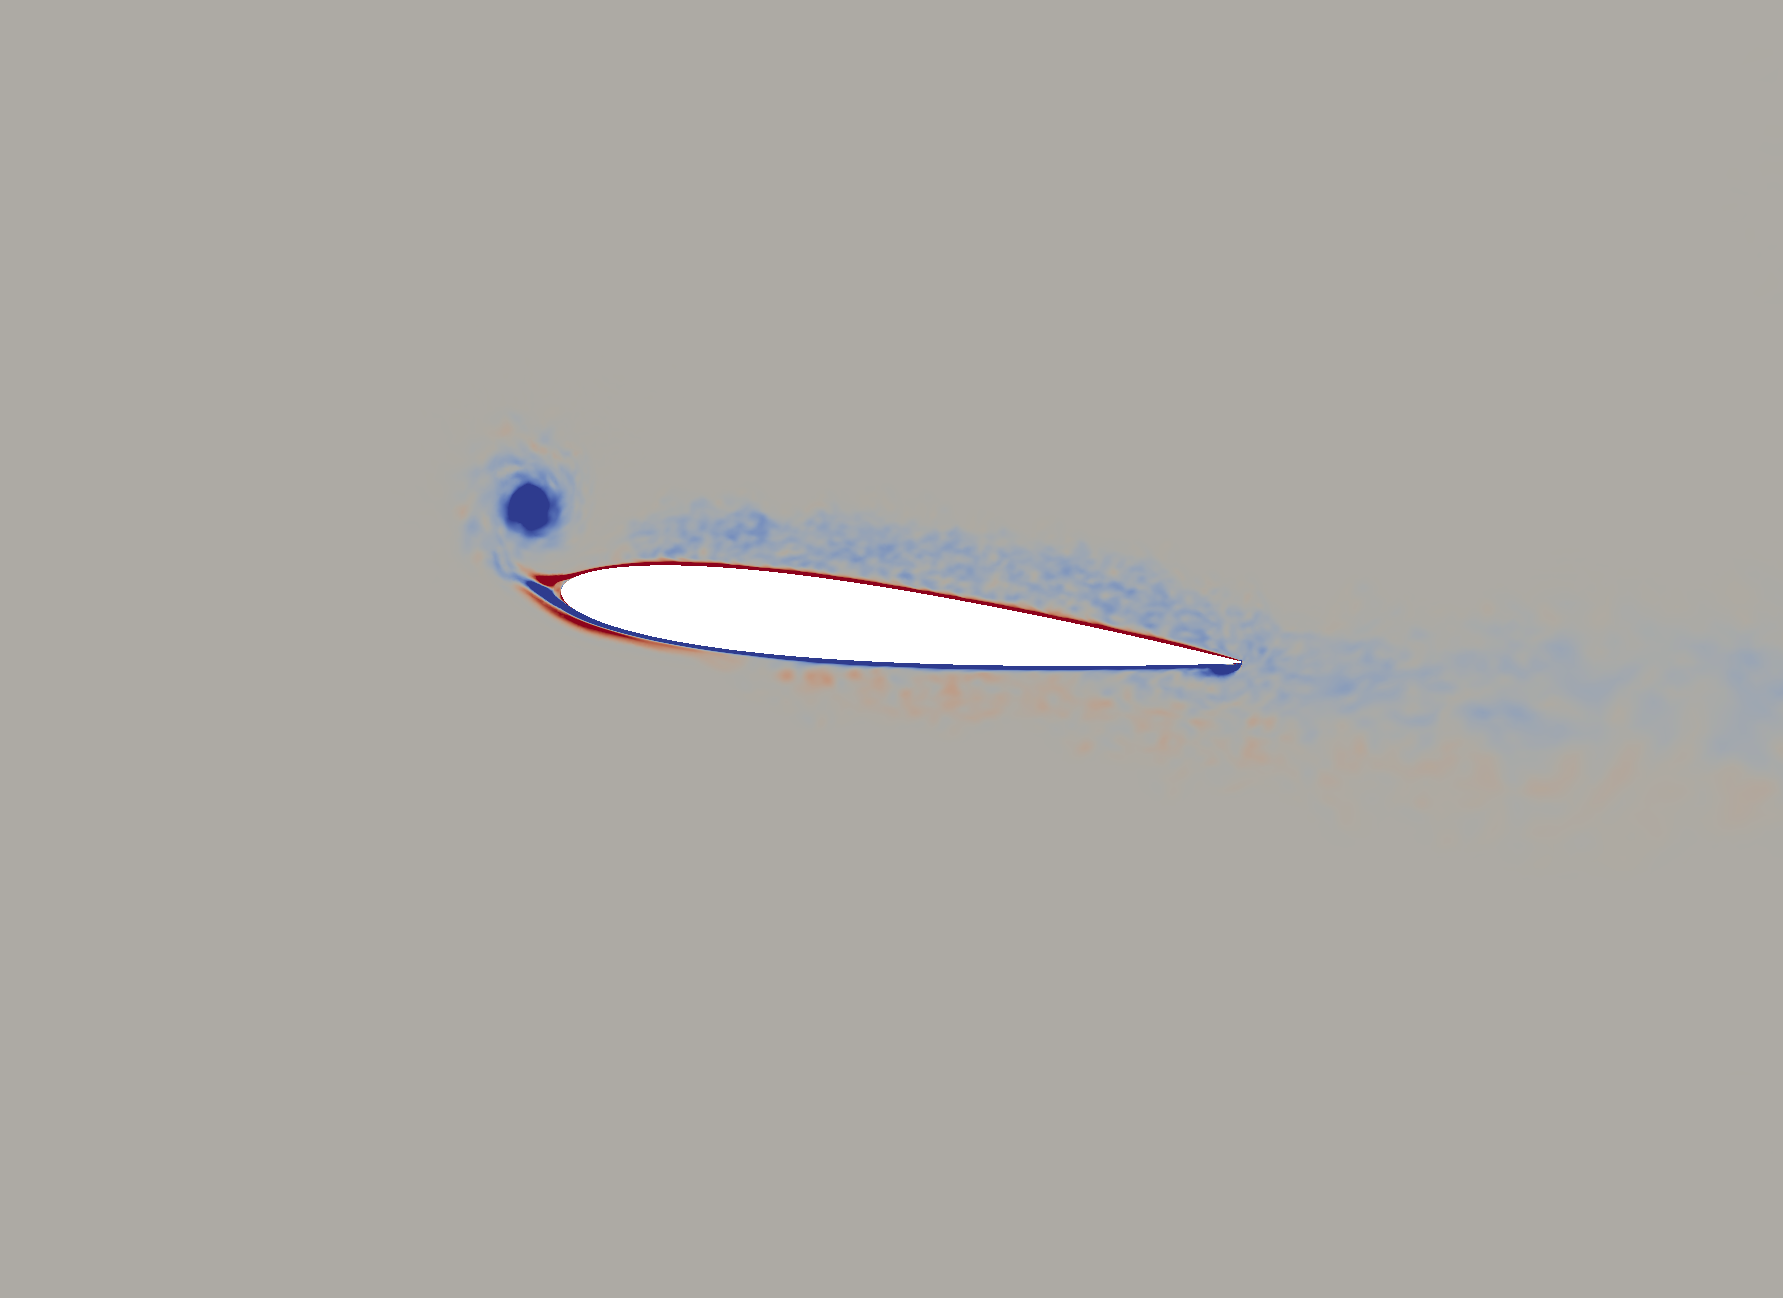
\includegraphics[width=1\textwidth]{figures/Vorticity_plots/Re_200k_1pt2/phase_255.png}
		\caption{$Re=2e5$, $\psi$ = $255^\circ$, $\tilde{t}=0.708$}
		\label{fig:Re_200k_1pt2_phi255}
	\end{subfigure}
	\begin{subfigure}[b]{0.32\textwidth}
		\centering
		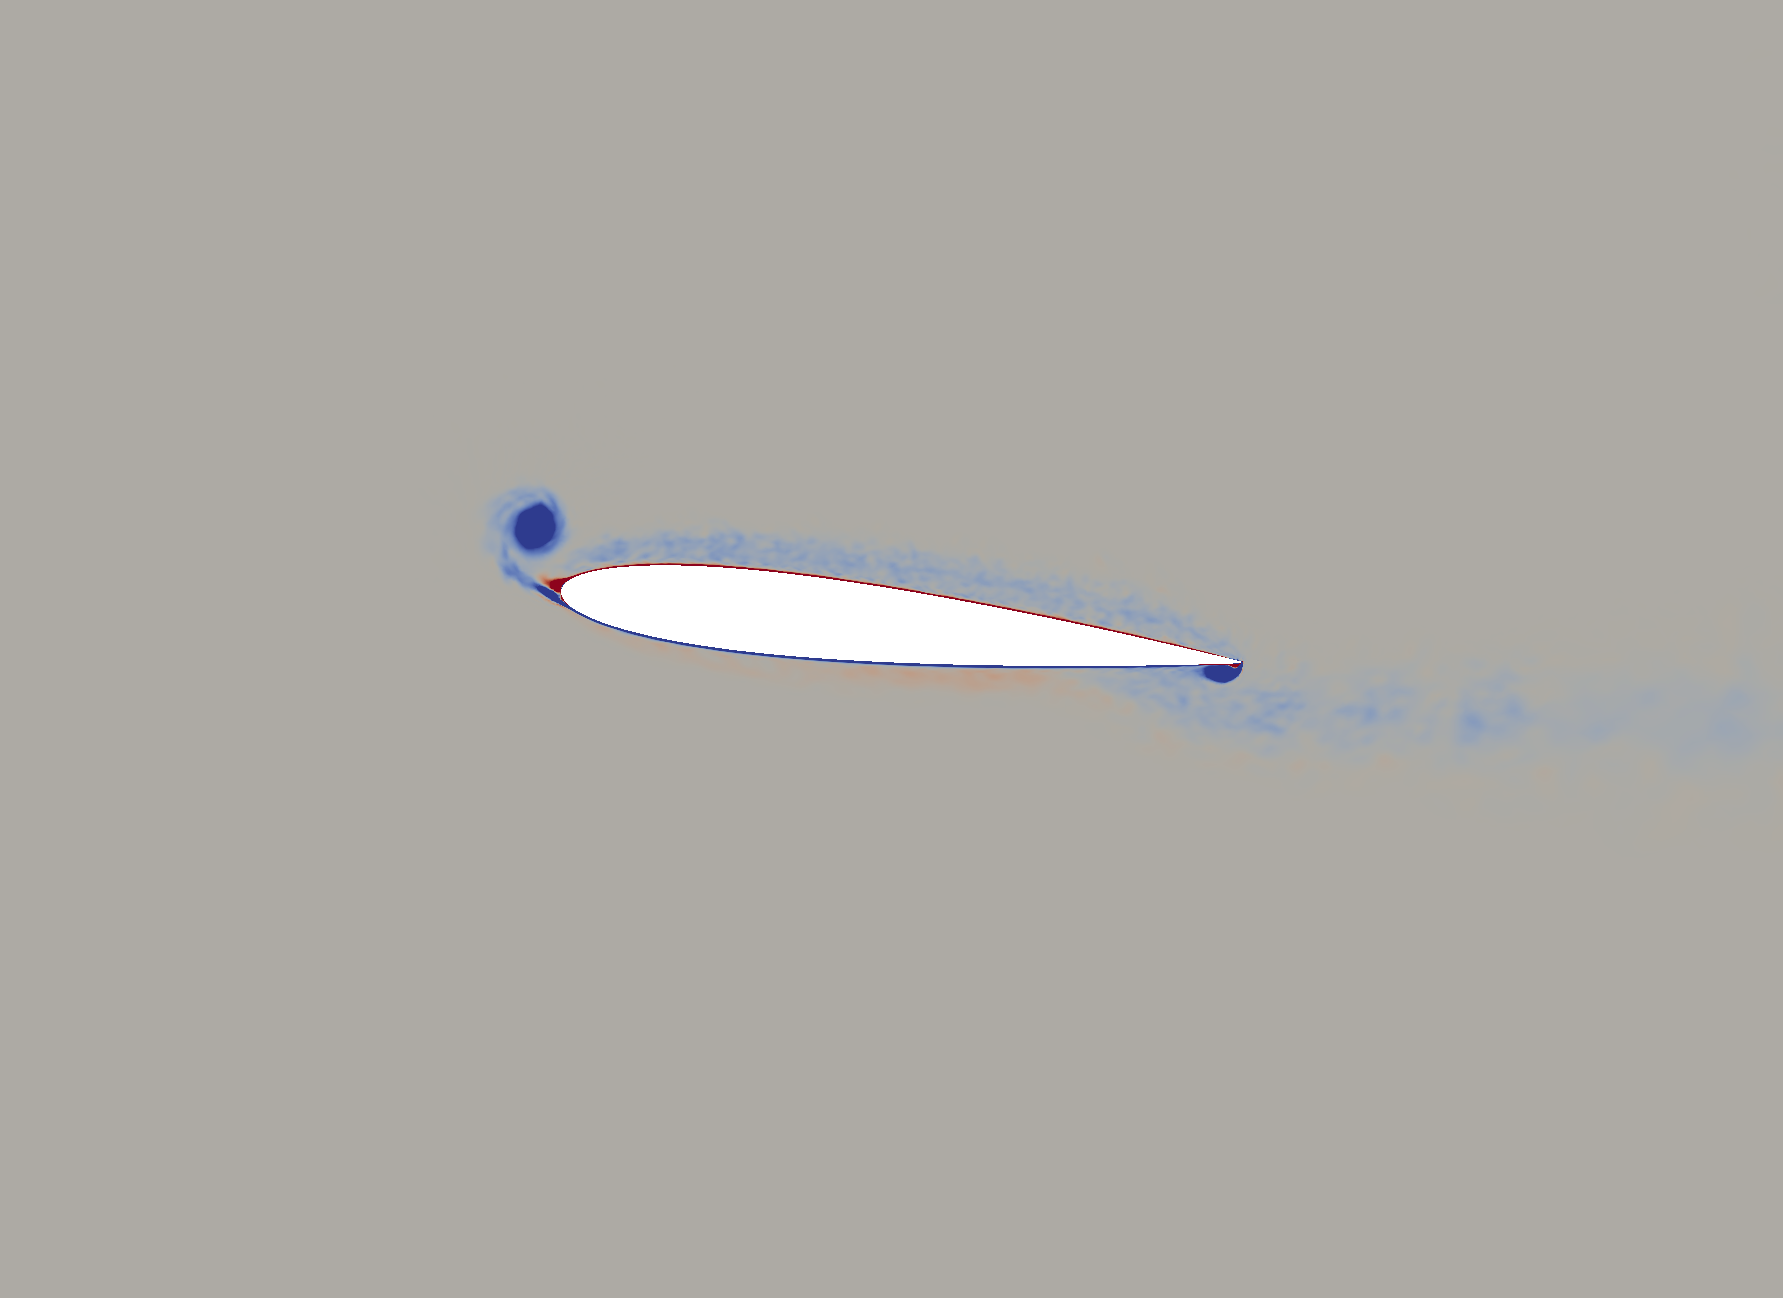
\includegraphics[width=1\textwidth]{figures/Vorticity_plots/Re_1m_1pt2/phase_255.png}
		\caption{$Re=1e6$, $\psi$ = $255^\circ$, $\tilde{t}=0.708$}
		\label{fig:Re_1m_1pt2_phi255}
	\end{subfigure}
	
	\caption{Spanwise vorticity at 8 different phases for $Re$=40,000 (left column), 200,000 (middle column) and 1,000,000 (right column) at $\mu_{sect}$ = 1.2}
%	\label{fig:vortScreen_1pt2}
\end{figure}


\begin{figure}[H]\ContinuedFloat
	\centering
	\begin{subfigure}[b]{0.32\textwidth}
		\centering
		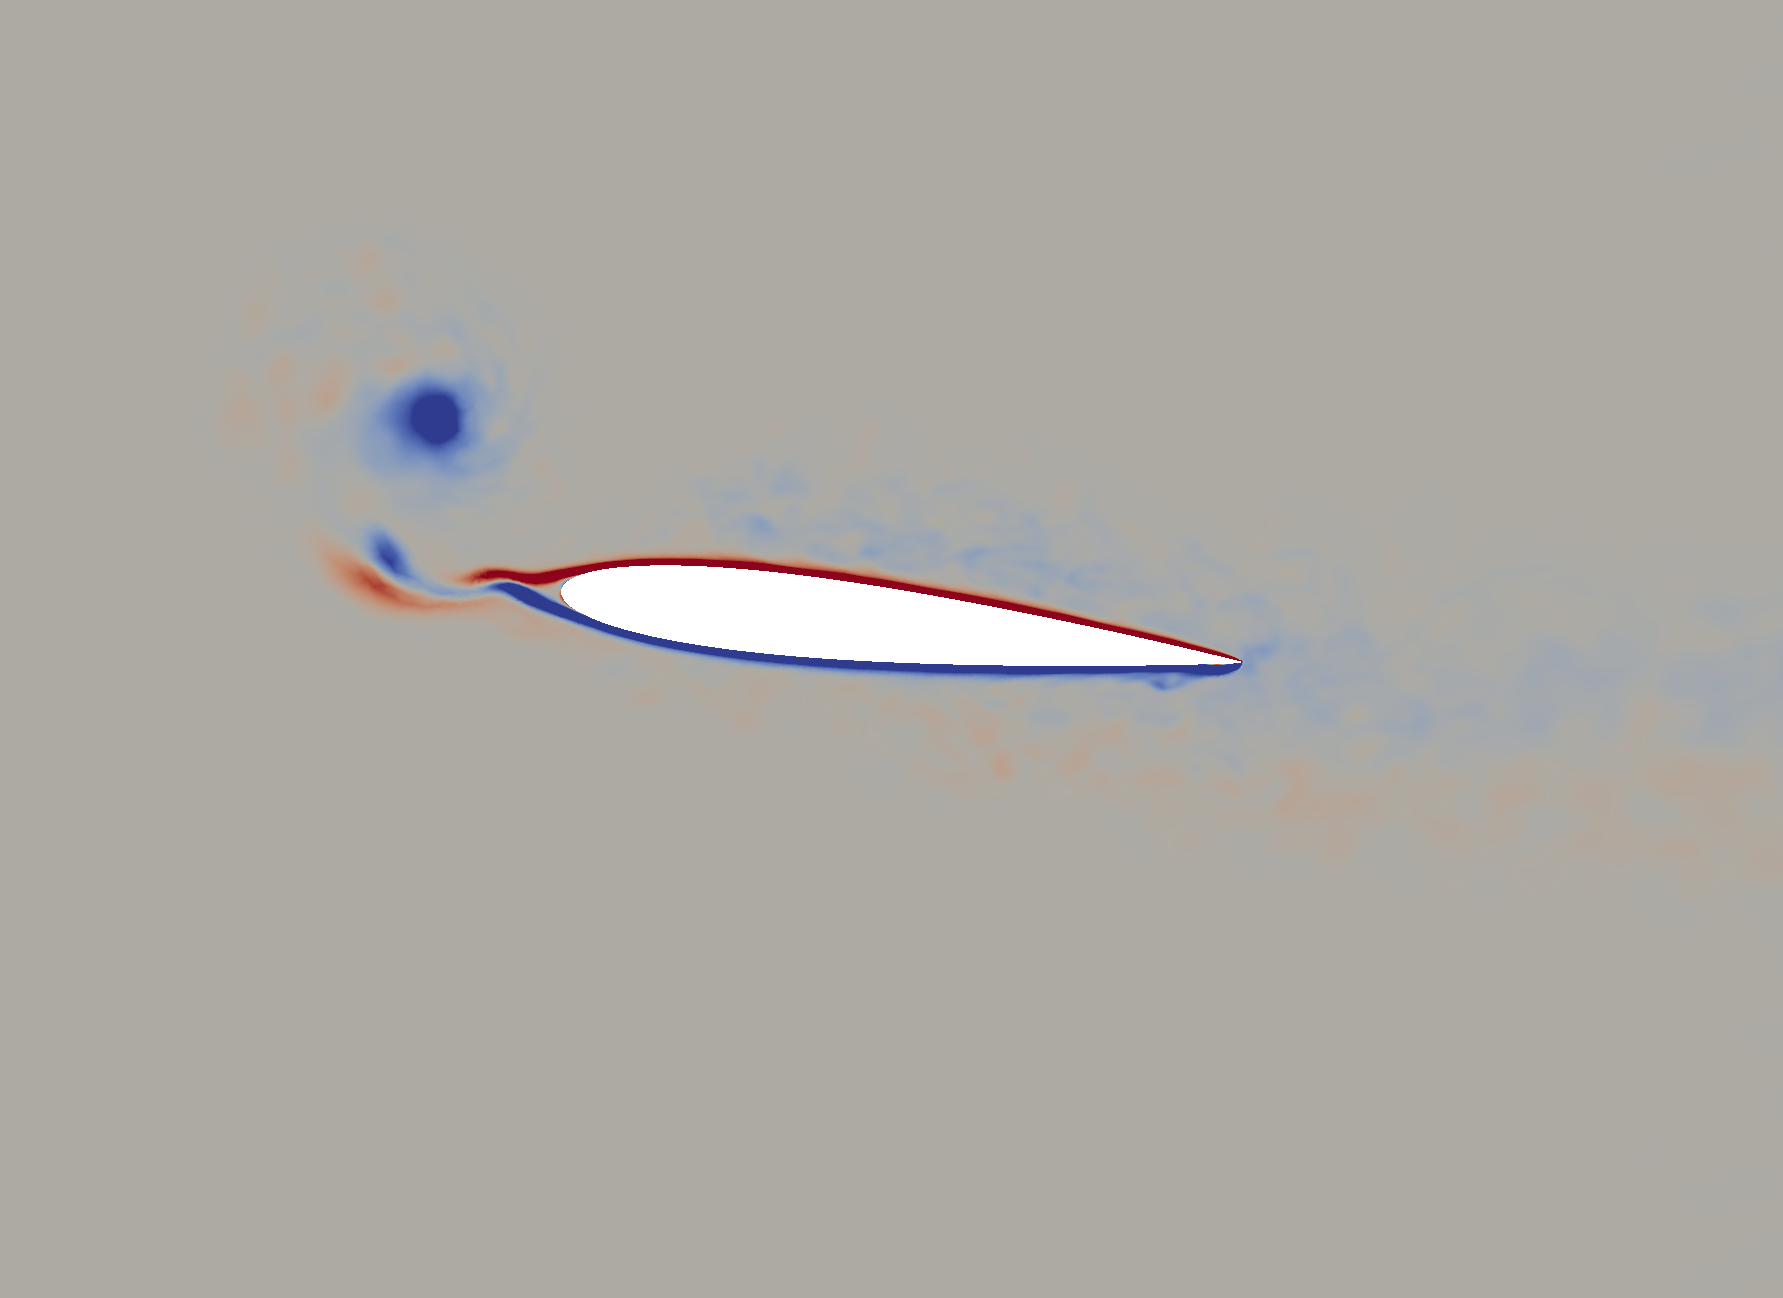
\includegraphics[width=1\textwidth]{figures/Vorticity_plots/Re_40k_1pt2/phase_270.png}
		\caption{$Re=4e4$, $\psi$ = $270^\circ$, $\tilde{t}=0.750$}
		\label{fig:Re_40k_1pt2_phi270}
	\end{subfigure}
	\begin{subfigure}[b]{0.32\textwidth}
		\centering
		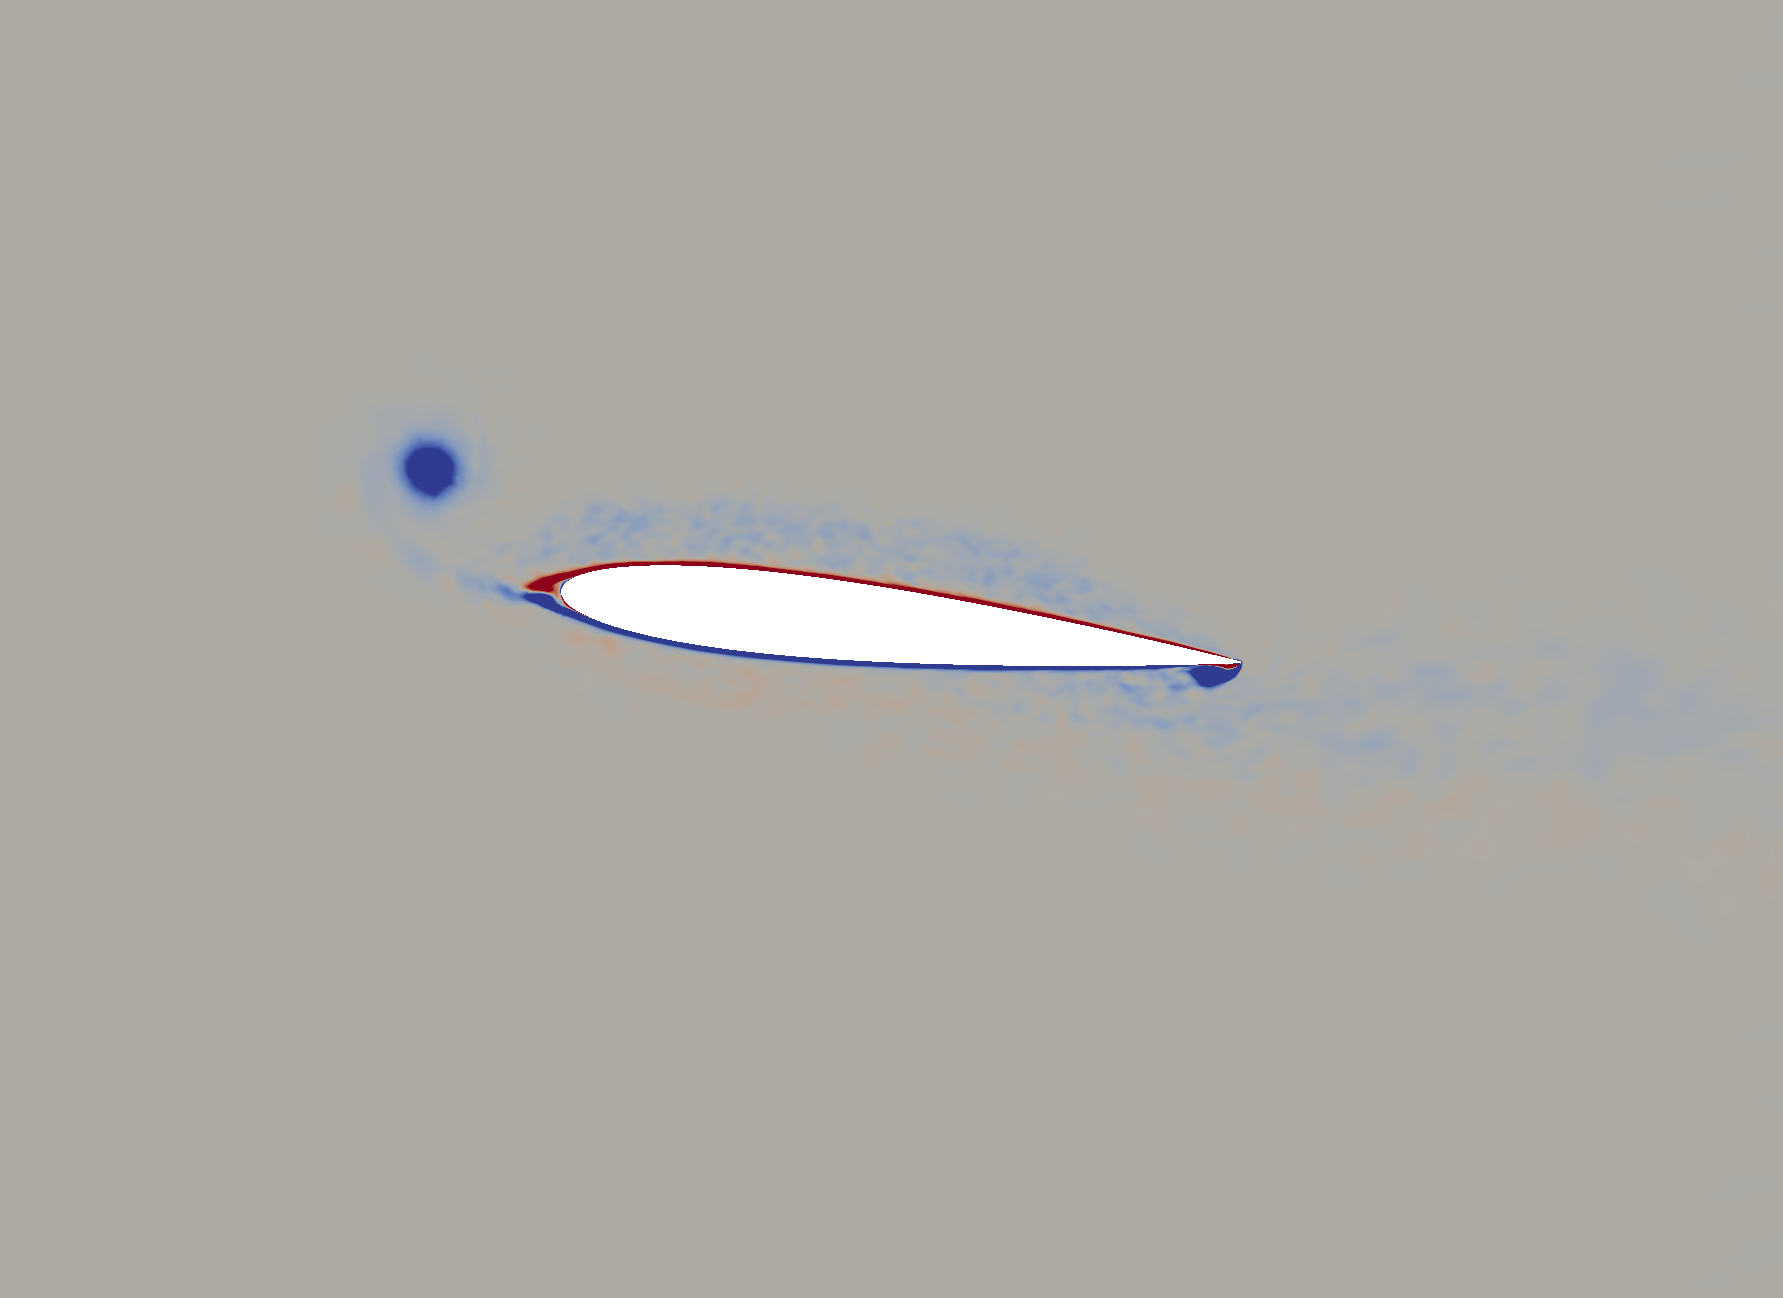
\includegraphics[width=1\textwidth]{figures/Vorticity_plots/Re_200k_1pt2/phase_270.png}
		\caption{$Re=2e5$, $\psi$ = $270^\circ$, $\tilde{t}=0.750$}
		\label{fig:Re_200k_1pt2_phi270}
	\end{subfigure}
	\begin{subfigure}[b]{0.32\textwidth}
		\centering
		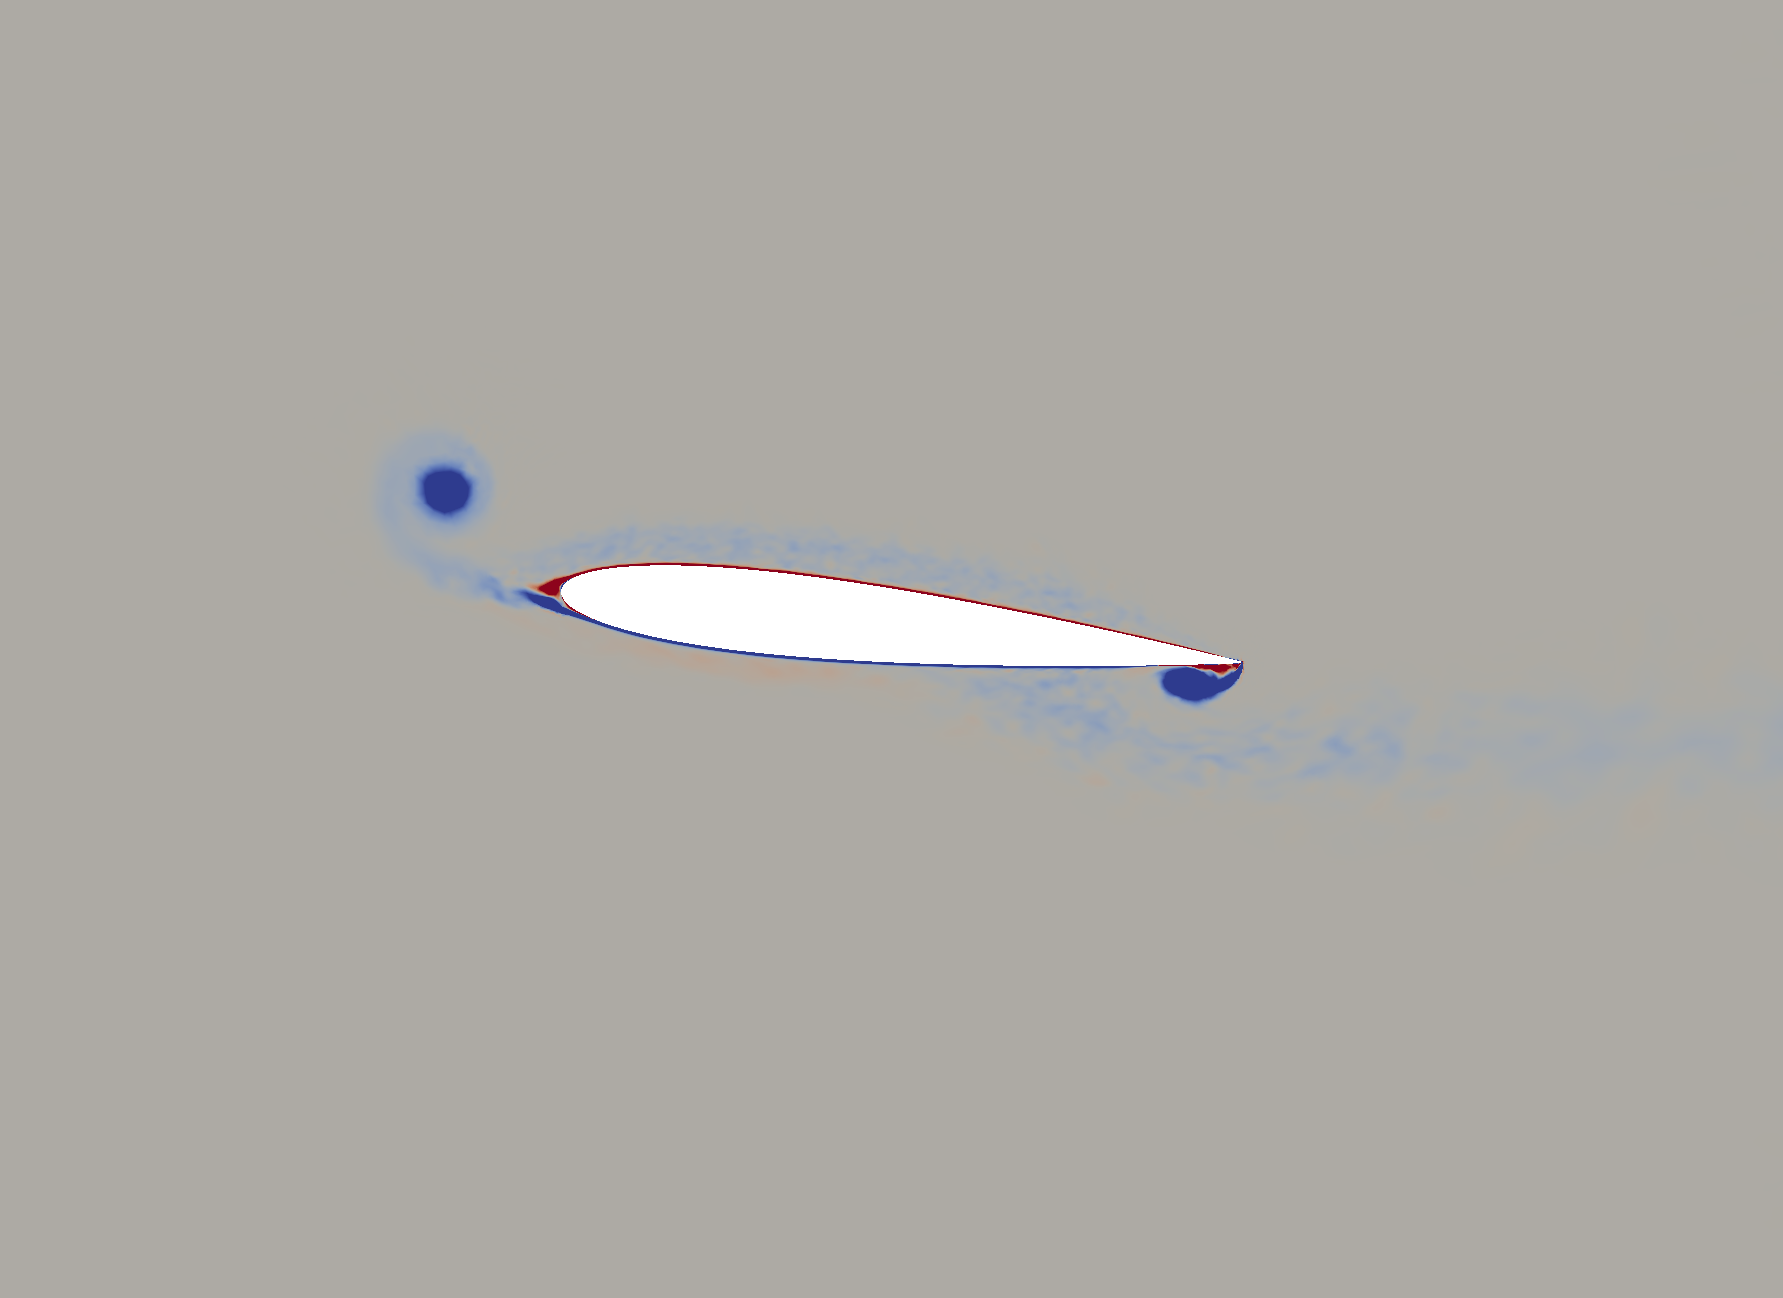
\includegraphics[width=1\textwidth]{figures/Vorticity_plots/Re_1m_1pt2/phase_270.png}
		\caption{$Re=1e6$, $\psi$ = $270^\circ$, $\tilde{t}=0.750$}
		\label{fig:Re_1m_1pt2_phi270}
	\end{subfigure}
	
	\begin{subfigure}[b]{0.32\textwidth}
		\centering
		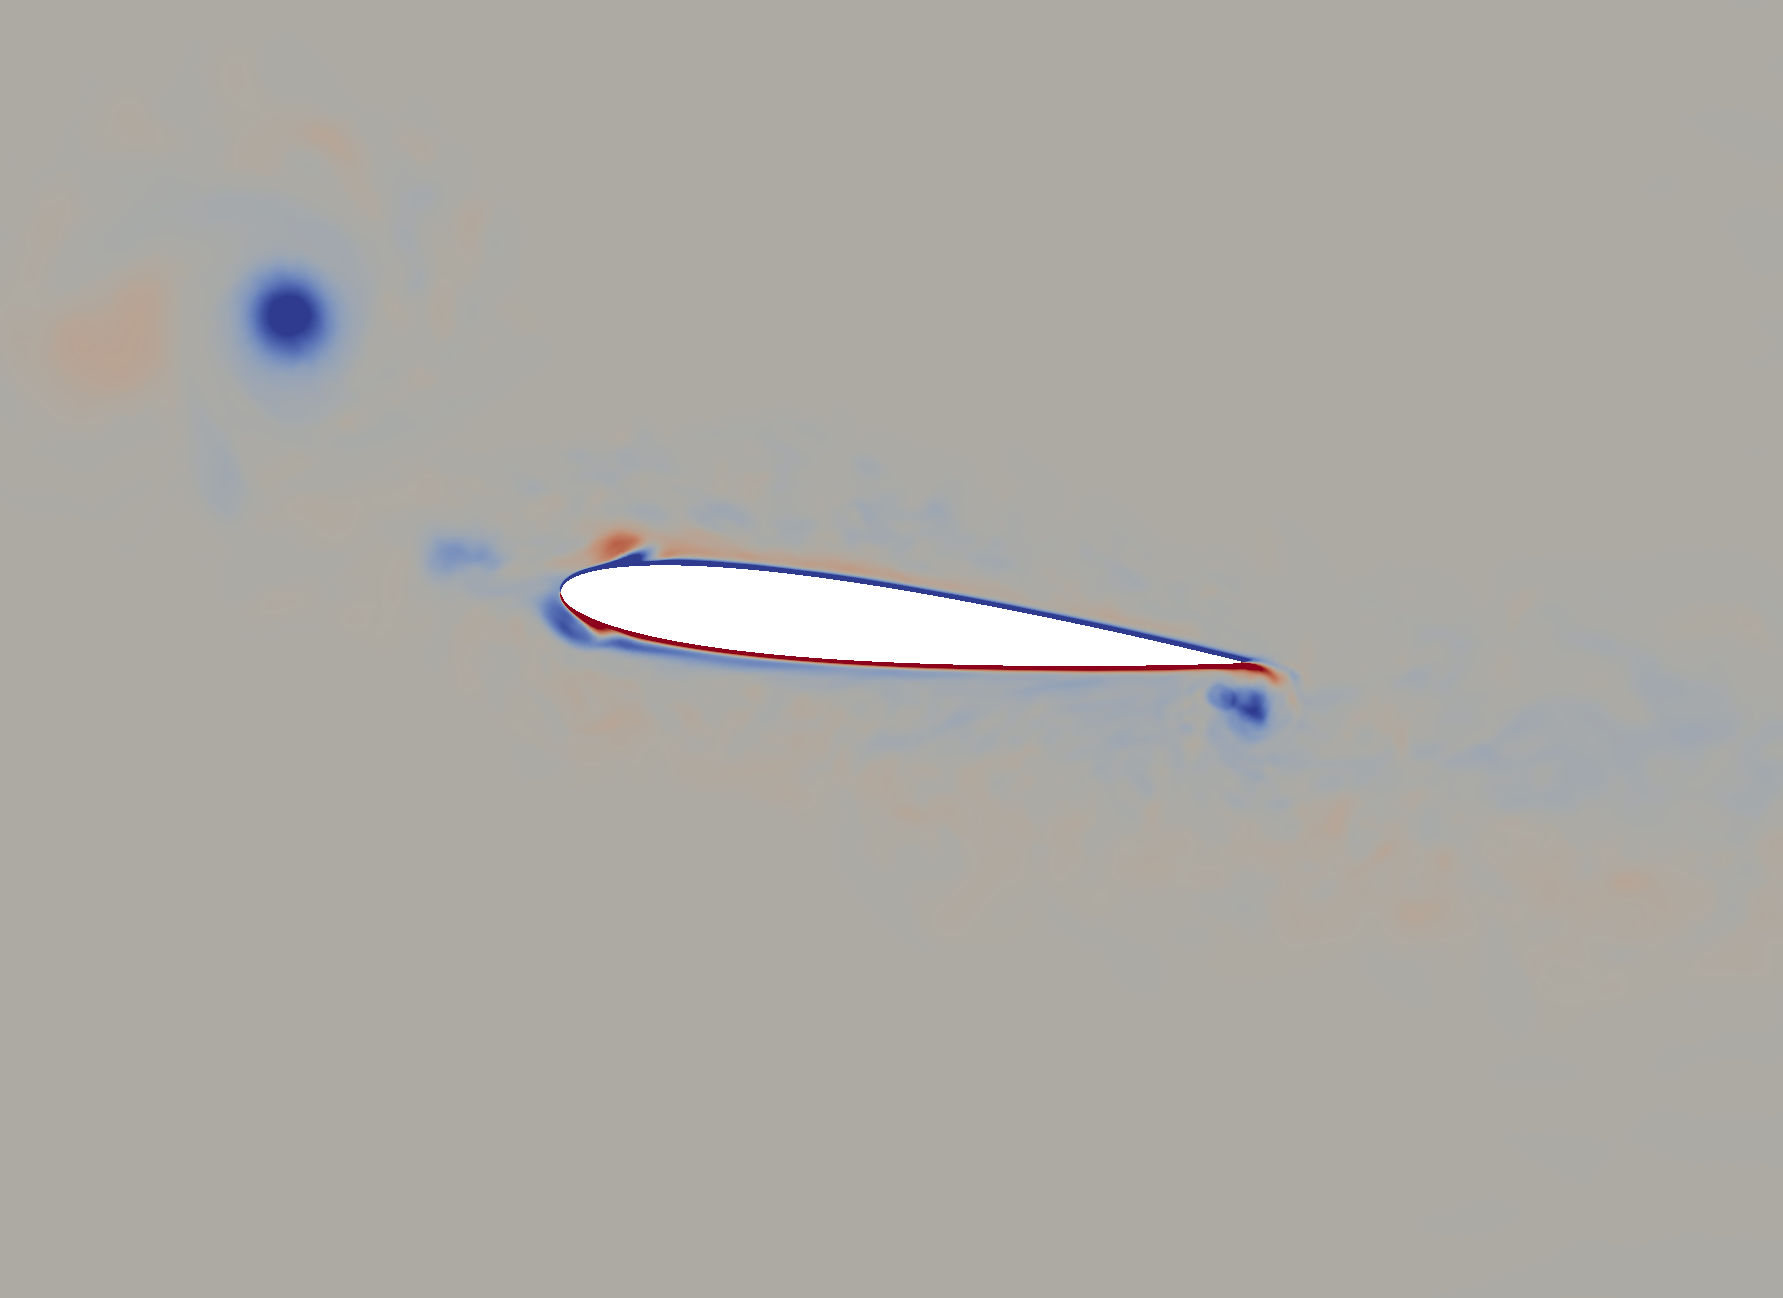
\includegraphics[width=1\textwidth]{figures/Vorticity_plots/Re_40k_1pt2/phase_315.png}
		\caption{$Re=4e4$, $\psi$ = $315^\circ$, $\tilde{t}=0.875$}
		\label{fig:Re_40k_1pt2_phi315}
	\end{subfigure}
	\begin{subfigure}[b]{0.32\textwidth}
		\centering
		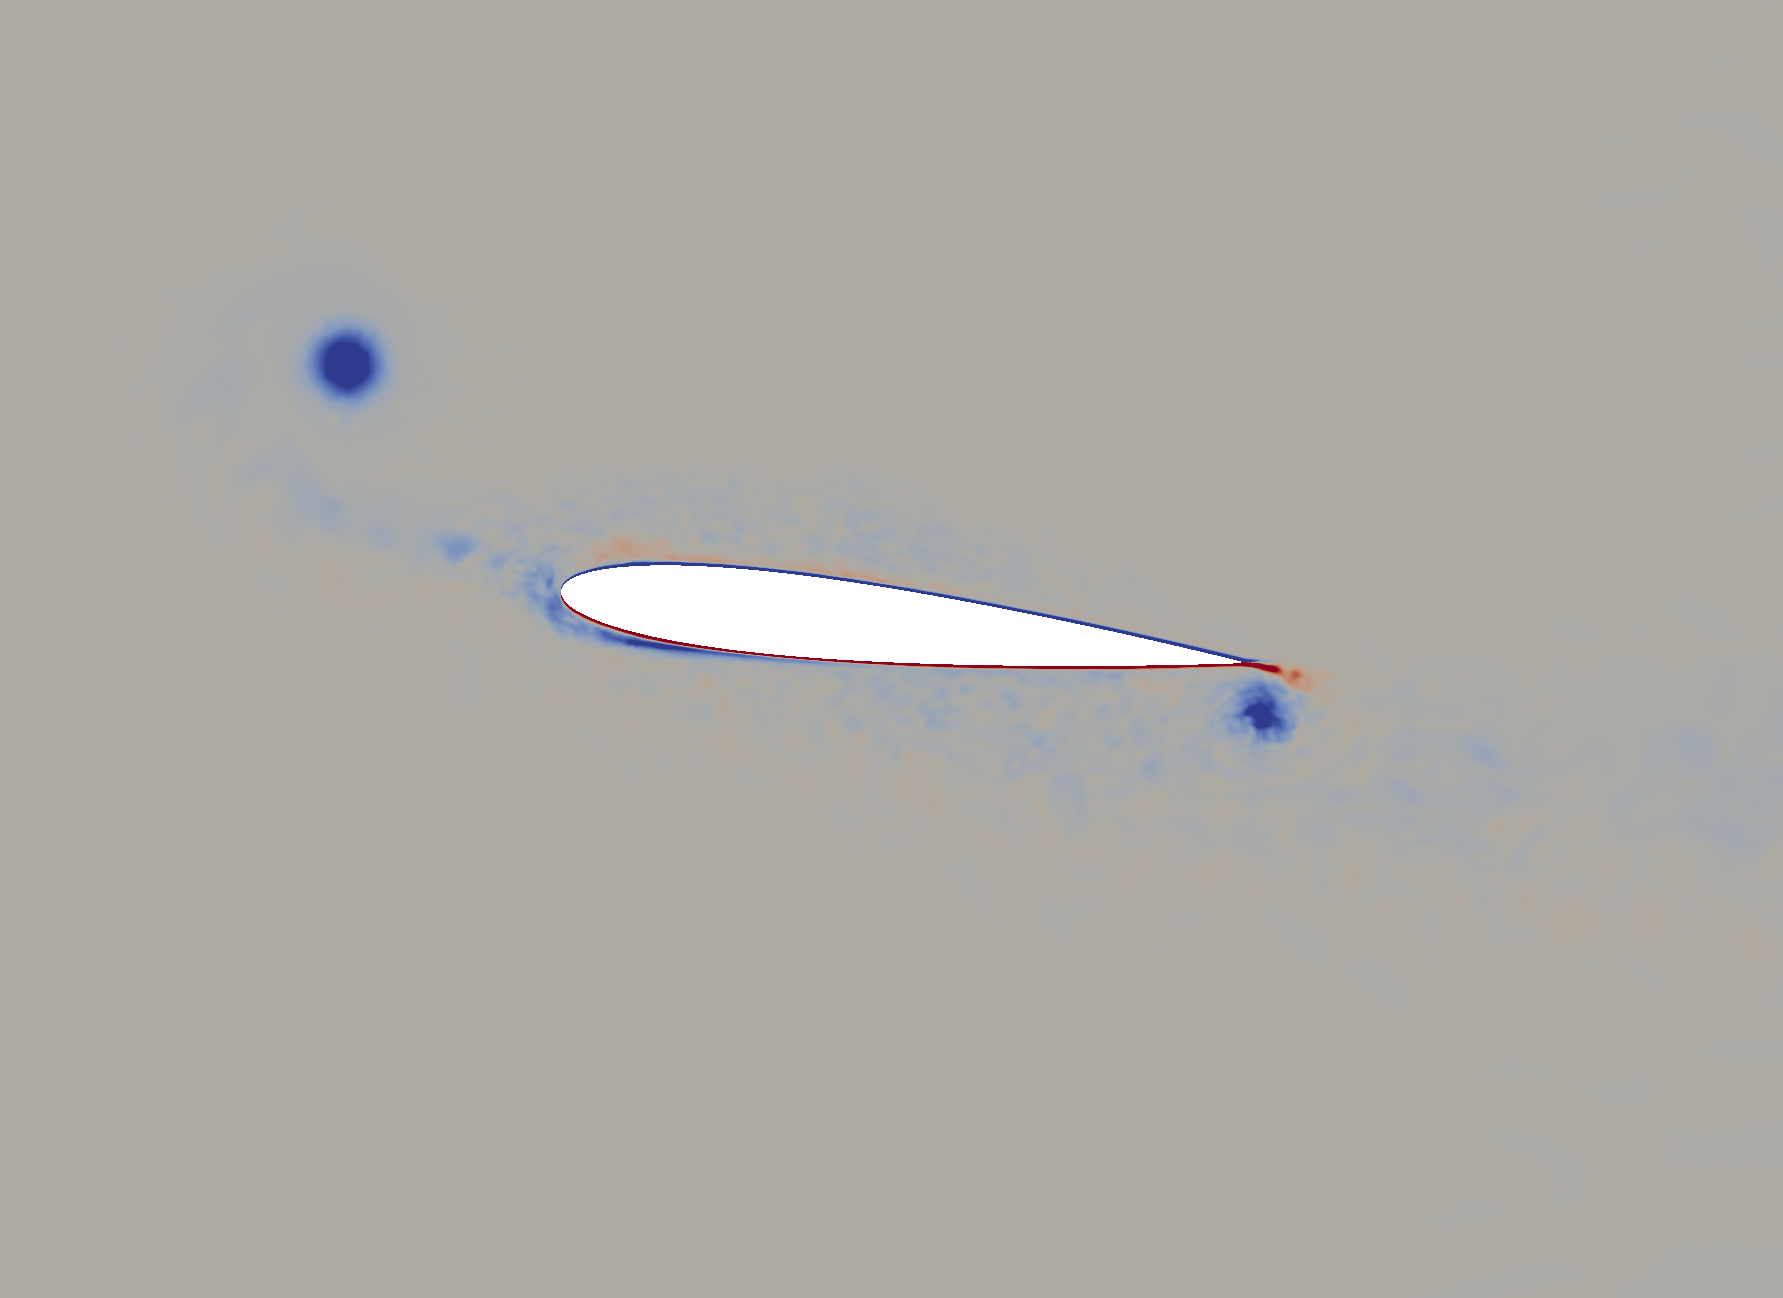
\includegraphics[width=1\textwidth]{figures/Vorticity_plots/Re_200k_1pt2/phase_315.png}
		\caption{$Re=2e5$, $\psi$ = $315^\circ$, $\tilde{t}=0.875$}
		\label{fig:Re_200k_1pt2_phi315}
	\end{subfigure}
	\begin{subfigure}[b]{0.32\textwidth}
		\centering
		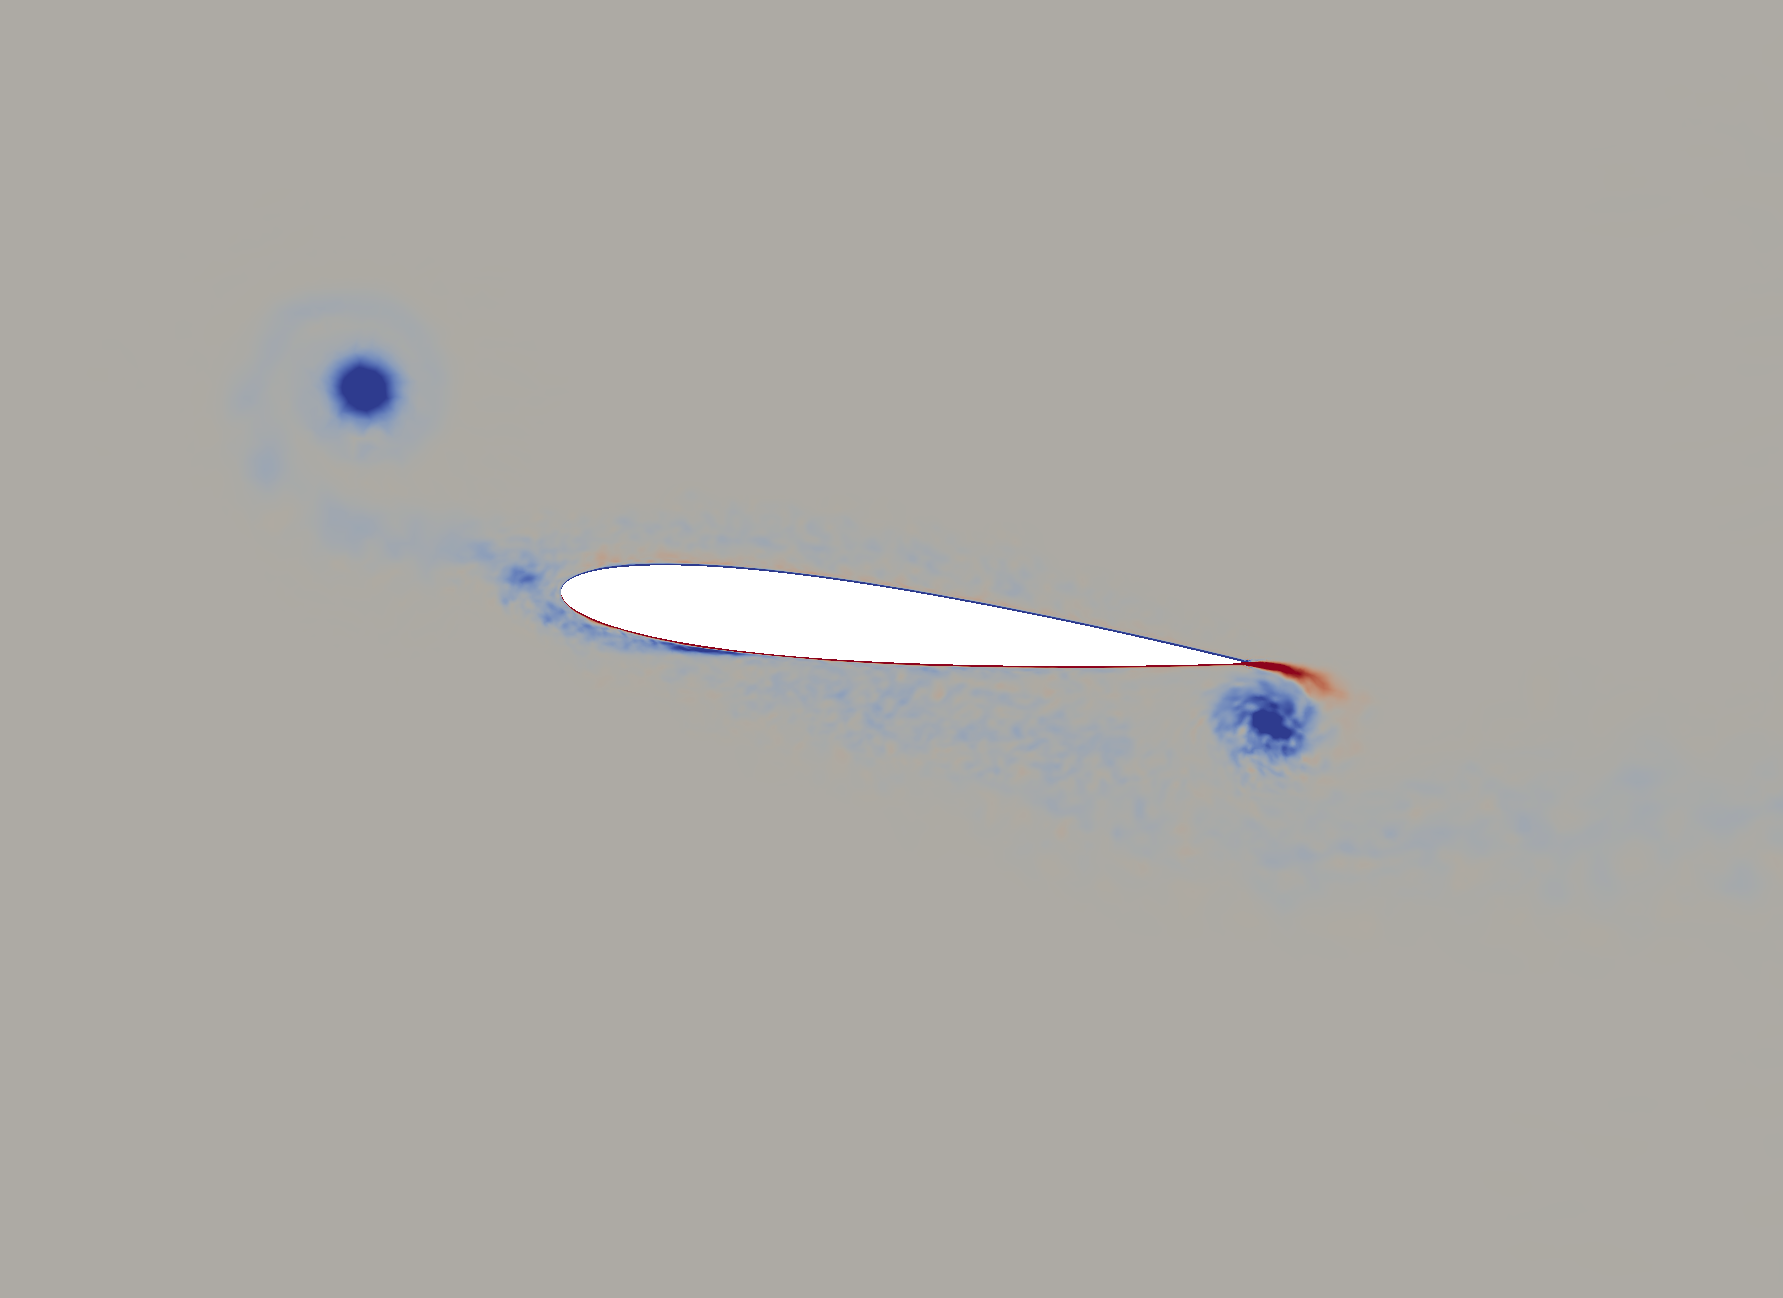
\includegraphics[width=1\textwidth]{figures/Vorticity_plots/Re_1m_1pt2/phase_315.png}
		\caption{$Re=1e6$, $\psi$ = $315^\circ$, $\tilde{t}=0.875$}
		\label{fig:Re_1m_1pt2_phi315}
	\end{subfigure}
	
	\begin{subfigure}[b]{0.32\textwidth}
		\centering
		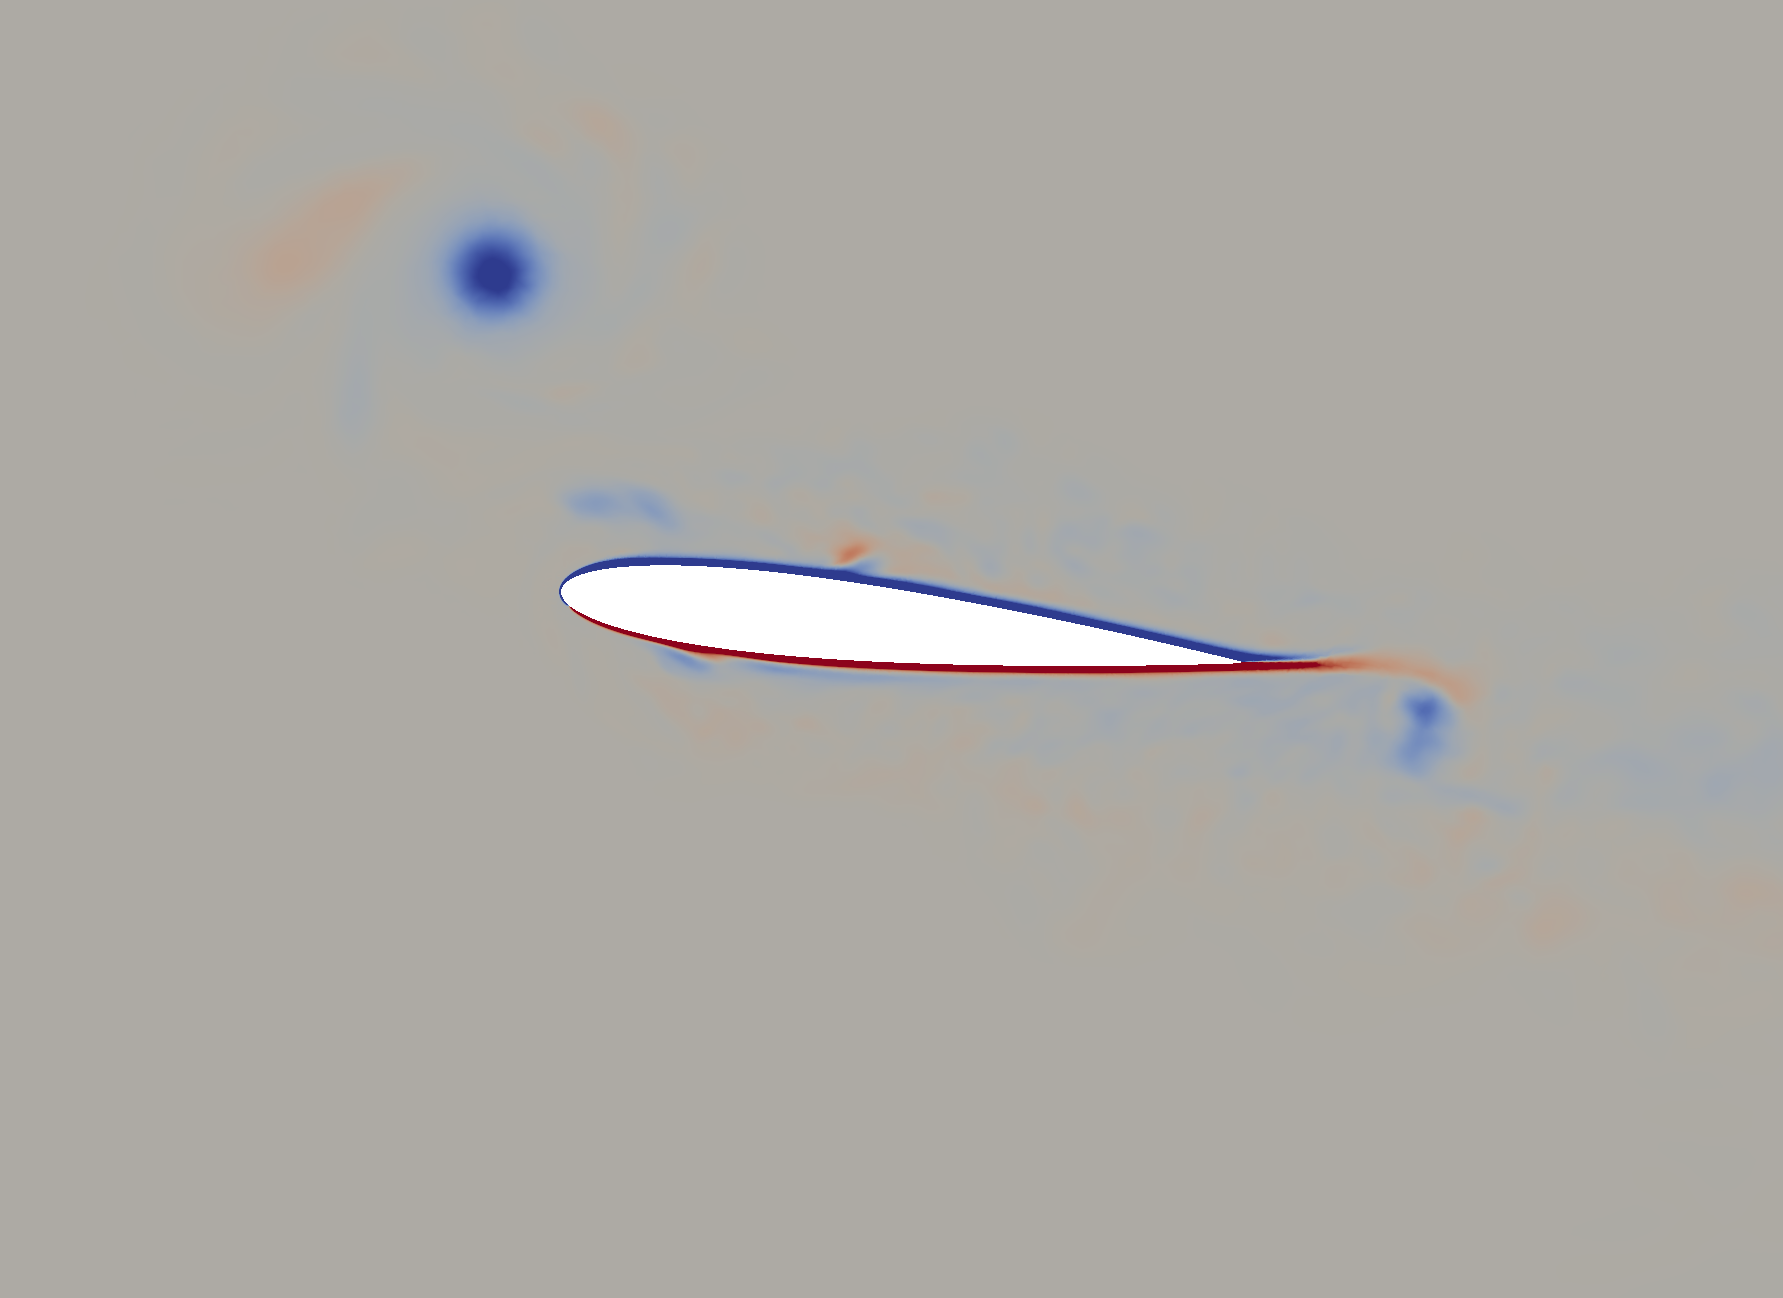
\includegraphics[width=1\textwidth]{figures/Vorticity_plots/Re_40k_1pt2/phase_330.png}
		\caption{$Re=4e4$, $\psi$ = $330^\circ$, $\tilde{t}=0.917$}
		\label{fig:Re_40k_1pt2_phi330}
	\end{subfigure}
	\begin{subfigure}[b]{0.32\textwidth}
		\centering
		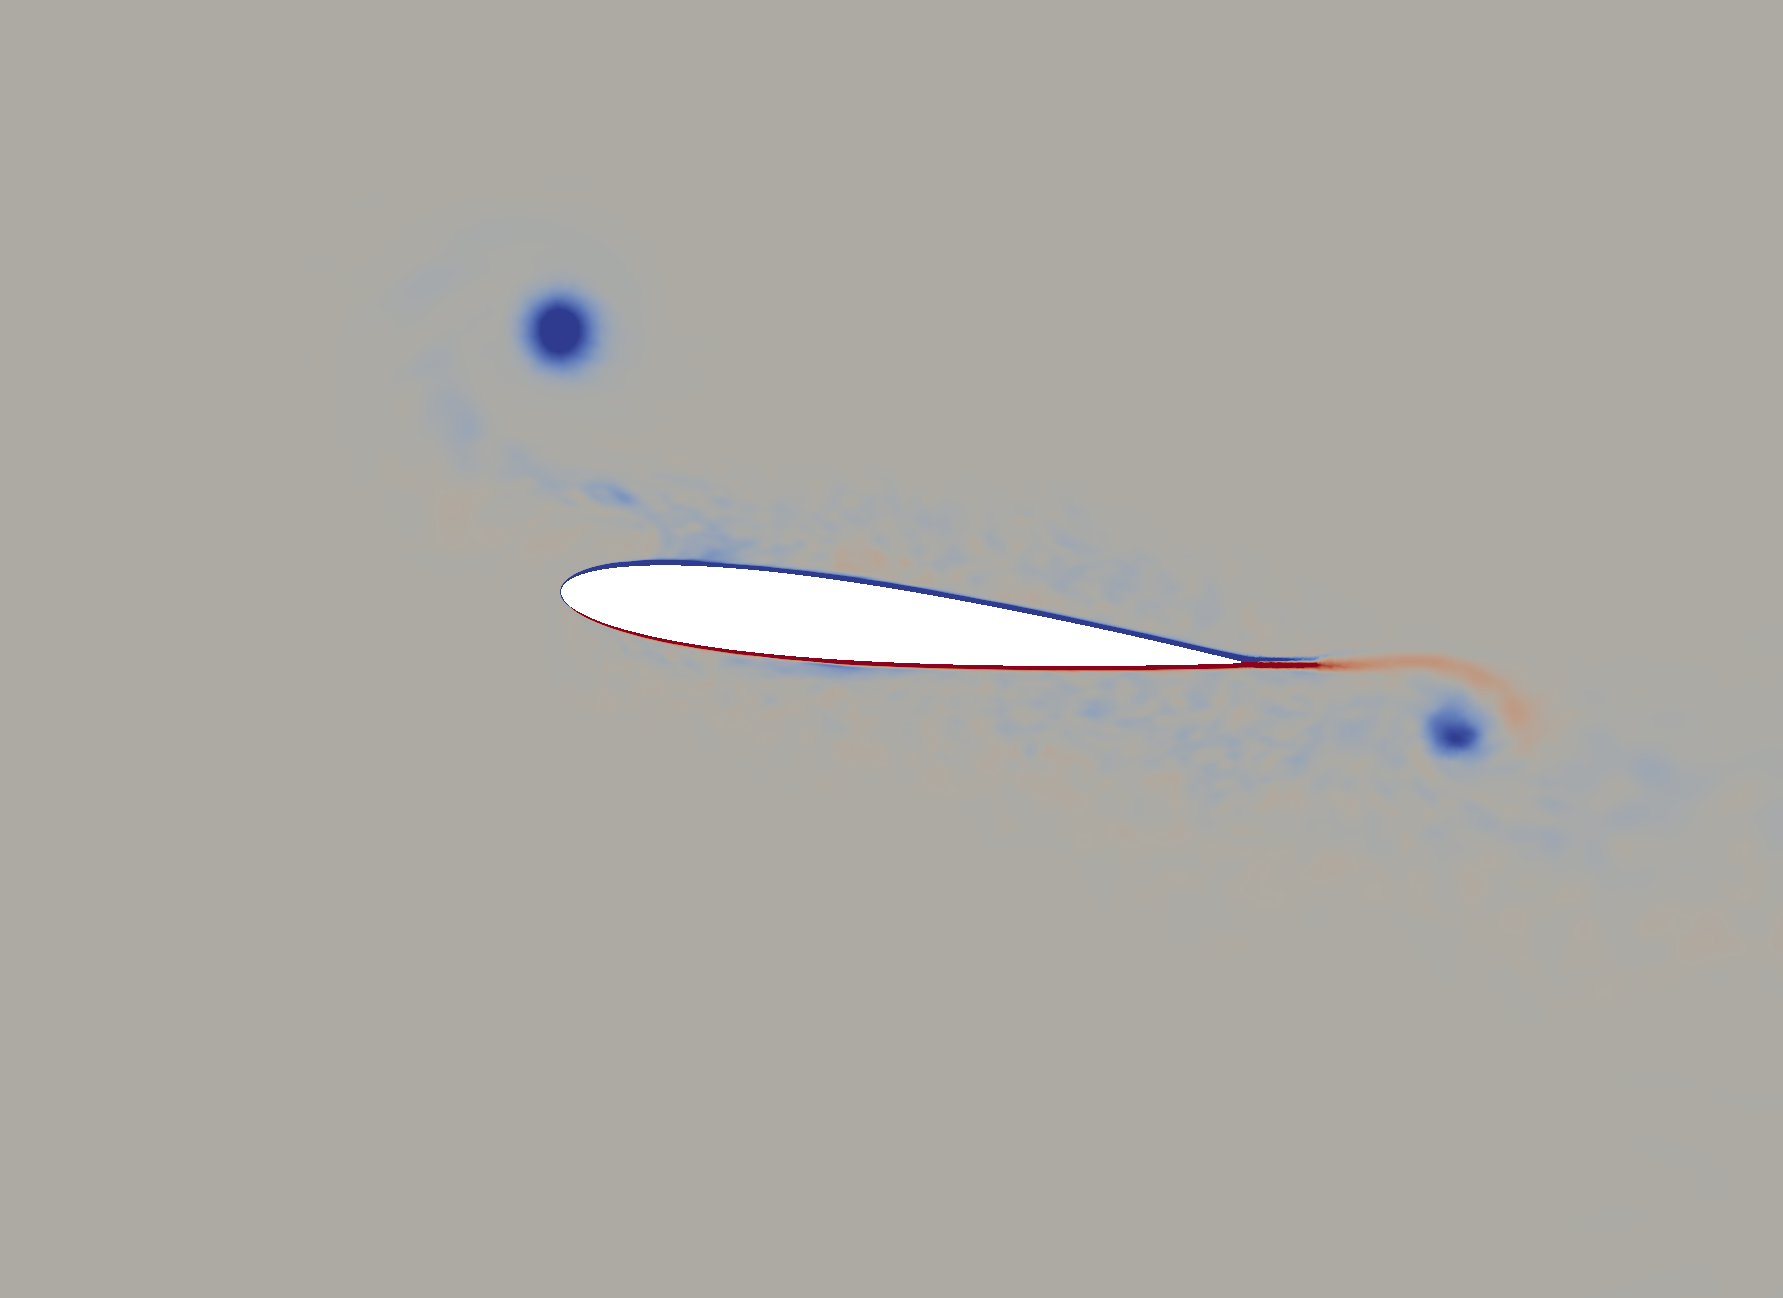
\includegraphics[width=1\textwidth]{figures/Vorticity_plots/Re_200k_1pt2/phase_330.png}
		\caption{$Re=2e5$, $\psi$ = $330^\circ$, $\tilde{t}=0.917$}
		\label{fig:Re_200k_1pt2_phi330}
	\end{subfigure}
	\begin{subfigure}[b]{0.32\textwidth}
		\centering
		\includegraphics[width=1\textwidth]{figures/Vorticity_plots/Re_1m_1pt2/phase_330.png}
		\caption{$Re=1e6$,$\psi$ = $330^\circ$, $\tilde{t}=0.917$}
		\label{fig:Re_1m_1pt2_phi330}
	\end{subfigure}	
	\begin{subfigure}[b]{0.32\textwidth}
		\centering
		\includegraphics[width=1\textwidth]{figures/Vorticity_plots/Re_40k_1pt2/phase_345.png}
		\caption{$Re=4e4$, $\psi$ = $345^\circ$, $\tilde{t}=0.958$}
		\label{fig:Re_40k_1pt2_phi345}
	\end{subfigure}
	\begin{subfigure}[b]{0.32\textwidth}
		\centering
		\includegraphics[width=1\textwidth]{figures/Vorticity_plots/Re_200k_1pt2/phase_345.png}
		\caption{$Re=2e5$, $\psi$ = $345^\circ$, $\tilde{t}=0.958$}
		\label{fig:Re_200k_1pt2_phi345}
	\end{subfigure}
	\begin{subfigure}[b]{0.32\textwidth}
		\centering
		\includegraphics[width=1\textwidth]{figures/Vorticity_plots/Re_1m_1pt2/phase_345.png}
		\caption{$Re=1e6$,$\psi$ = $345^\circ$, $\tilde{t}=0.958$}
		\label{fig:Re_1m_1pt2_phi345}
	\end{subfigure}
	
	\caption{Spanwise vorticity at 8 different phases for $Re$=40,000 (left column), 200,000 (middle column) and 1,000,000 (right column) at $\mu_{sect}$ = 1.2}
	\label{fig:vortScreen_1pt2}
\end{figure}

\subsection{LEV Evolution}
\label{sec:LEV}

%TODO: Use pics from presentation

LEV detection and tracking is performed using the procedure developed in this work, see Section \ref{sec:LEV_detect_track}. LEV position with respect to the leading edge of the airfoil is presented in Figure~\ref{fig:LEV_location_LE_airfoil}.
In the $\mu_{sect}=1.0$ case, the initial position of the LEV (i.e., position at formation) gets closer to the leading edge as the Reynolds number is increased.
Further, LEV remains closest to the airfoil over the cycle for the highest Reynolds number of $Re$=1,000,000 (i.e., note the vertical position of the LEV).
On the other hand, LEV initially moves to the left (towards the geometric leading edge) from its initial position for the lowest Reynolds number of $Re$=40,000.
In the $\mu_{sect}=1.2$ case also, similar trends are observed.
However, at the higher advance ratio the LEV initially moves to the left past the geometric leading edge for each Reynolds number.
This is expected since the relative flow velocity becomes negative (or a reversed flow condition is obtained) at $\mu_{sect}=1.2$.

Figure \ref{fig:LEV_size} presents the size or core radius ($r_c$) of the LEV for all six cases.
We note that in simulations the data was recorded at every $\Delta \psi = 15^\circ$ starting at $\psi$=$15^\circ$.
For each case the LEV is formed at about $\tilde{t}=0.6$ or later.
The LEV size is higher for the lowest Reynolds number of $Re$=40,000 for both advance ratios of $\mu_{sect}$=1.0 and 1.2.
This is expected since the boundary layer is thicker for $Re$=40,000 and the resulting separated shear layer rolls up into a larger LEV.
The LEV size is very similar for the other two higher Reynolds numbers at $\mu_{sect}$=1.0 and 1.2.
In the $\mu_{sect}$=1.0 case, the LEV increases in size till about $\tilde{t}=0.75$ to 0.8 and subsequently seem to plateau or increase in size relatively slowly.
Towards the end of the cycle, the LEV size is predicted to be about 8\% of the chord for $Re$=40,000 at $\mu_{sect}$=1.0, and about 6\% for $Re$=200,000 and 1,000,000 at $\mu_{sect}$=1.0.
In the $\mu_{sect}$=1.2 case, the LEV increases in size throughout the cycle and towards the end of the cycle reaches about a similar size as the $\mu_{sect}$=1.0 case for each Reynolds number. Note that such a quantification of LEV evolution, based on feature/vortex detection and tracking procedure, is also useful for feature-based adaptivity, which is discussed in Section \ref{sec:feature_based_strat}.

\begin{figure}[H]
	\begin{subfigure}{0.5\textwidth}
		\includegraphics[width=1\textwidth]{figures/LEV_size_lambda_1pt0.png}
		\caption{$\mu_{sect} = 1.0$}
		\label{fig:LEV_size_lambda_1p0}
	\end{subfigure}
 	\begin{subfigure}{0.5\textwidth}
	\includegraphics[width=1\textwidth]{figures/LEV_size_lambda_1pt2.png}
	\caption{$\mu_{sect} = 1.2$}
	\label{fig:LEV_size_lambda_1p2}
	\end{subfigure}
 	\caption{LEV evolution: LEV size for $Re$=40,000 (green line with open triangles), 200,000 (red line with closed circles) and 1,000,000 (blue line with open circles) at $\mu_{sect}$=1.0 and 1.2}
 	\label{fig:LEV_size}
\end{figure}




%TODO: indicate we consider Re=40k and 200k for adaptive LES and carefully investigate mesh convergence. this was done for cost savings since LEV exhibits a similar behavior for Re=200k and Re=1m cases.

\begin{figure}[H]
	\begin{subfigure}{0.5\textwidth}
		\includegraphics[width=1\textwidth]{figures/LEV_location_lambda_1pt0}
		\caption{$\mu_{sect} = 1.0$}
		\label{fig:LEV_location_lambda_1p0}
	\end{subfigure}
	\begin{subfigure}{0.5\textwidth}
		\includegraphics[width=1\textwidth]{figures/LEV_location_lambda_1pt2}
		\caption{$\mu_{sect} = 1.2$}
		\label{fig:LEV_location_lambda_1p2}
	\end{subfigure}
 	\caption{LEV evolution: LEV position (with respect to the leading edge of the airfoil) for $Re$=40,000 (green line with open triangles), 200,000 (red line with closed circles) and 1,000,000 (blue line with open circles) at $\mu_{sect}$=1.0 and 1.2}
	\label{fig:LEV_location_LE_airfoil}
\end{figure}

In Figure \ref{fig:LEV_delta_x}, the horizontal displacement of the LEV with respect to the ground is presented.
The displacement is taken about the initial position when the LEV is formed, i.e., the displacement is zero at the initial position.
Again, as the Reynolds number increases the LEV is formed later in the cycle (for a given advance ratio) while as the advance ratio increases it is formed earlier in the cycle (for a given Reynolds number).

An important aspect to note in Figure \ref{fig:LEV_delta_x} is that the horizontal displacement of the LEV follows a straight line for each case and is parallel among all cases.
The slope of the horizontal displacement in each case is remarkably close to the free-stream velocity, i.e., the LEV is advected in the horizontal direction at the free-stream velocity.

\begin{figure}[H]
	\begin{subfigure}{0.5\textwidth}
		\includegraphics[width=1\textwidth]{figures/LEV_deltax_lambda_1pt0.png}
		\caption{$\mu_{sect} = 1.0$}
		\label{fig:LEV_deltax_lambda_1p0}
	\end{subfigure}
	\begin{subfigure}{0.5\textwidth}
		\includegraphics[width=1\textwidth]{figures/LEV_deltax_lambda_1pt2.png}
		\caption{$\mu_{sect} = 1.2$}
		\label{fig:LEV_deltax_lambda_1p2}
	\end{subfigure}
	\caption{LEV evolution: LEV displacement (in the horizontal direction) for $Re$=40,000 (green line with open triangles), 200,000 (red line with closed circles) and 1,000,000 (blue line with open circles) at $\mu_{sect}$=1.0 and 1.2}
	\label{fig:LEV_delta_x}
\end{figure}
